\documentclass[12pt,titlepage]{article}
\usepackage[authoryear]{natbib}
\bibliographystyle{genetics}
\usepackage{amsfonts}
\usepackage{amsmath}
\usepackage{amssymb}
\usepackage{graphicx}
\usepackage{rotating}
\usepackage{marginnote}
\usepackage{color}
\usepackage{fullpage}

% Added by Simon:
\usepackage[normalem]{ulem}

\newcommand{\gc}[1]{{\em \color{green} #1}}
\newcommand{\sa}[1]{{\color{black} #1}}
\newcommand{\plr}[1]{{\em \color{green} (#1)}}
\newcommand{\E}{\mathbb{E}}
\renewcommand{\P}{\mathbb{P}}
\newcommand{\half}{\tfrac{1}{2}}

\newcommand{\wbar}{\overline{w}}
% New commands added by Simon:
\newcommand{\fis}{F_{\mathrm{IS}}}
\newcommand{\fit}{F_{\mathrm{IT}}}
\newcommand{\fst}{F_{\mathrm{ST}}}
\newcommand{\Wbar}{\overline{W}}

\definecolor{rev1}{rgb}{1, 0, 0}

\begin{document}

\title{Notes on Population Genetics}
\author{Graham Coop$^{1}$ \\
\small $^1$ Department of Evolution and Ecology \& Center for Population Biology,\\
\small University of California, Davis.\\
\small To whom correspondence should be addressed: \texttt{gmcoop@ucdavis.edu}\\
\small This work is licensed under a Creative Commons Attribution 3.0 Unported License.\\
\small http://creativecommons.org/licenses/by/3.0/ \\
\small i.e. you are free to reuse and remix this work, but please include an attribution to the original.
}

\date{}
\maketitle

\tableofcontents

\newpage
\section{Allele and genotype frequencies}

\subsection{Allele frequencies}
Consider a diploid autosomal locus segregating at two alleles ($A_1$ and $A_2$). Let $N_{11}$ and $N_{12}$ be the number of $A_1A_1$ homozygotes and $A_1A_2$ heterozygotes, respectively. Moreover, let $N$ be the total number of diploid individuals in the population. We can then define the relative frequencies of $A_1A_1$ and $A_1A_2$ genotypes as $f_{11} = N_{11}/N$ and $f_{12} = N_{12}/N$, respectively. The frequency of allele $A_1$ in the population is then given by
\begin{equation}
p = \frac{2 N_{11} + N_{12}}{2N} = f_{11} + \frac{1}{2} f_{12}. % Modified by Simon
\end{equation}
Note that this holds independently of Hardy--Weinberg proportions and equilibrium [see below]. The frequency of the alternate allele ($A_2$) is then just $q=1-p$.

\subsection{Hardy--Weinberg proportions}

Imagine a population mating at random with respect to genotypes, i.e.\
no inbreeding, no population structure, no sex differences in allele frequencies. The frequency of allele $A_1$ in the population at the time of reproduction is $p$. An $A_1A_1$ genotype is made by reaching out into our population and independently drawing two $A_1$ alelle gametes to form a zygote. Therefore, the probability that an individual is an $A_1A_1$ homozygote is $p^2$. This probability is also the expected frequency of the $A_1A_1$ homozygote in the population. The expected frequency of the three possible genotypes is
%\begin{table}[htp!]
\begin{center}
\begin{tabular}{|ccc|}
\hline
$f_{11}$ & $f_{12}$ & $f_{22}$ \\
\hline
$p^2$ & $2pq$ & $q^2$ \\
\hline
\end{tabular}\,.
\end{center}
%\caption{\textbf{Hardy Weinberg}} \label{table:HWE}
%\end{table}
Note that we only need to assume random mating with
respect to our alleles in order for these expected frequencies to hold,
as long at $p$ is the frequency of the $A_1$ allele in the population at
the time when gametes fuse.


%%%ADD A comment about WF sampling here!
%% Also add a question about Poisson offspring number.

\begin{figure}
\begin{center}
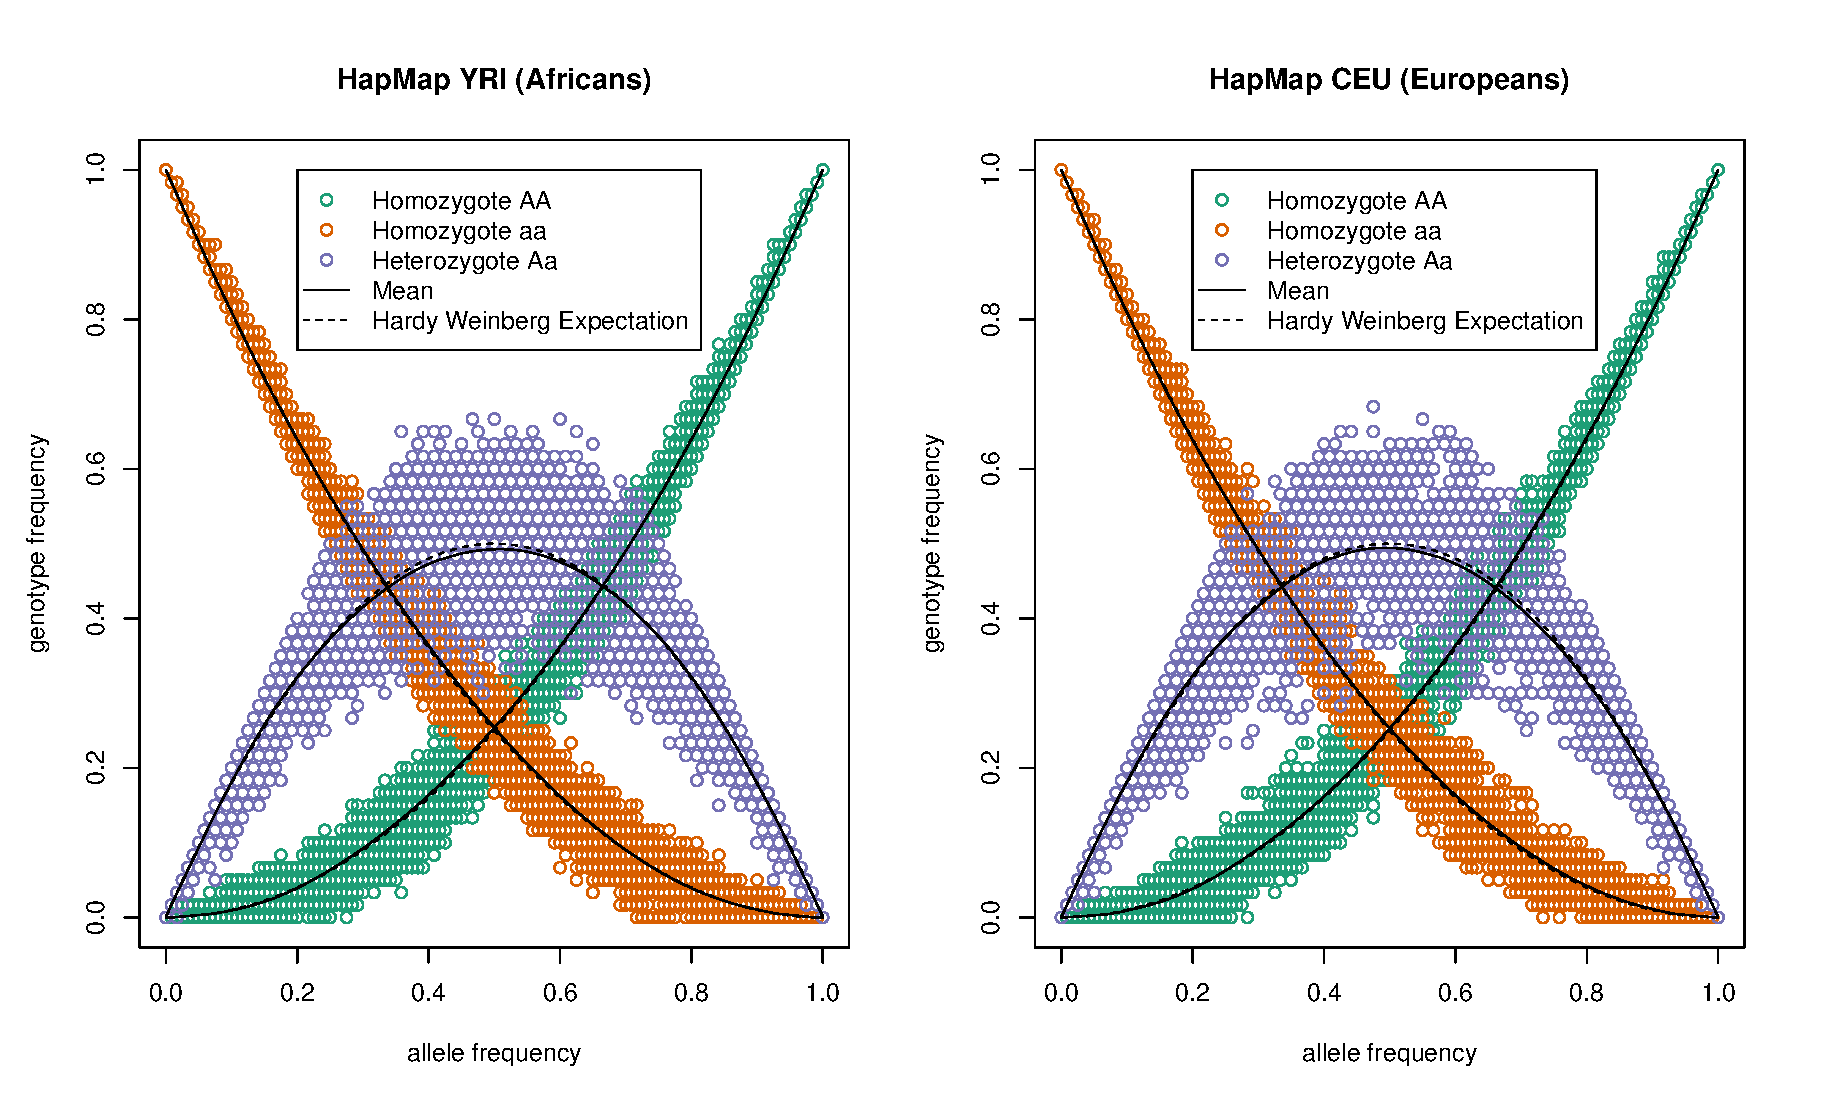
\includegraphics[width=0.8 \textwidth]{Figs/CEU_YRI_separately_HWE.eps}
\end{center}
\end{figure}


\begin{figure}
\begin{center}
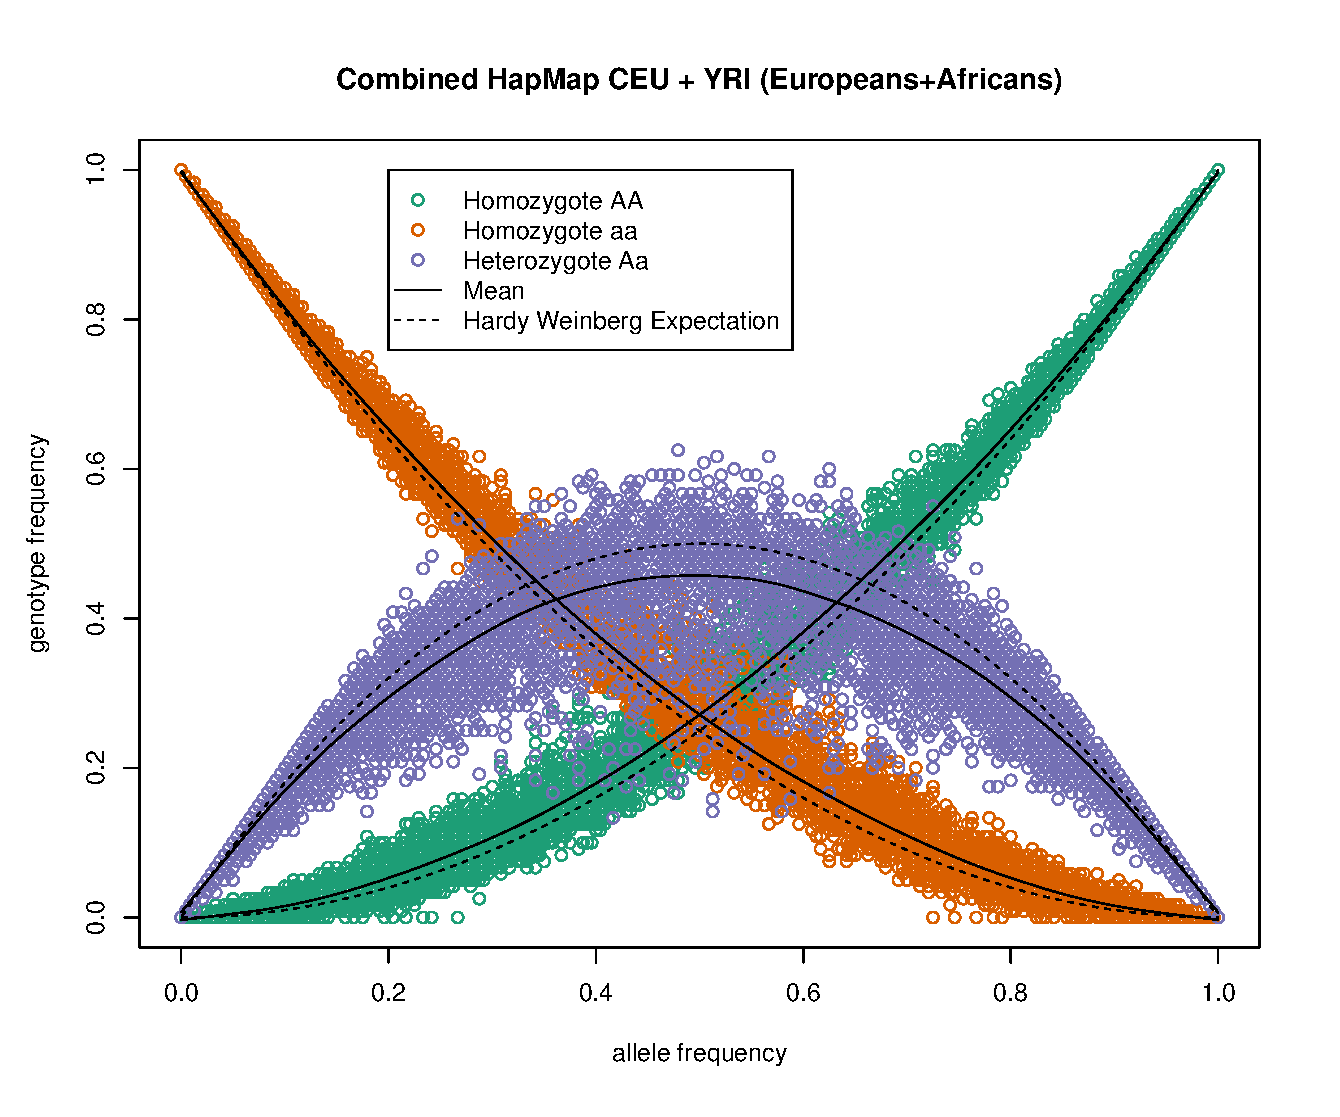
\includegraphics[width=0.5 \textwidth]{Figs/CEU_YRI_together_HWE.eps}
\end{center}
\end{figure}


%Figs/QT1.eps


\subsection{Coefficient of kinship}
We will define two alleles to be identical by descent if they are
identical due to a common ancestor in the past few generations. For the moment, we ignore mutation, and we will be more precise about what we mean by `past few generations' later on. For example, parent and child share exactly
one allele identical by descent at a locus, assuming that the two
parents of the child are randomly mated individuals from the population.\\

A key quantity is the probability that our pair of individuals share
0, 1, or 2 alleles identical by descent. We denote these probabilities
by $r_0$, $r_1$, and $r_2$ respectively. See Table \ref{table:IBDprobs} for
some examples. \\

One summary of relatedness that will be important is the probability that two alleles picked at random, one from each of the two different individuals $i$ and $j$, are identical by descent. We call this quantity the coefficient of kinship of individuals $i$ and $j$, and denote it by $F_{ij}$. It is calculated as
\begin{equation}
F_{ij}= 0 \times r_0 + \frac{1}{4} r_1  + \frac{1}{2} r_2. 
\label{eqn:coeffkinship}
\end{equation}

The coefficient of kinship will appear multiple times, in both our discussion of
inbreeding and in the context of phenotypic resemblance between relatives.\\

\begin{table}
\begin{center}
\begin{tabular}{| l | c c c c|}
\hline
Relationship (i,j)$^{*}$ & $r_0$ & $r_1$ & $r_2$ & $F_{ij}$\\
\hline
parent--child & 0 & 1 & 0 & 1/4\\
full siblings & 1/4 & 1/2 & 1/4 & 1/4\\
identical (monzygotic) twins  & 0 & 0 & 1  & 1/2 \\
$1^{st}$ cousins & 3/4 & 1/4 & 0 & 1/16\\
\hline
\end{tabular}
\end{center}
\caption{Probability that two individuals of a given relationship share 0, 1, or 2 alleles
identical by descent. $^{*}$ assuming this is the only relationship
the pair of individuals share (above that expected from randomly
sampling individuals from the population). } \label{table:IBDprobs}
\end{table}

\subsection{Inbreeding}
We can define an inbred individual as an individual whose parents are
more closely related to each other than two random individuals drawn
from some reference population.  \\

When two related individuals produce an offspring, that individual can
receive two alleles that are identical by descent, i.e.\ they
can be homozygous by descent (sometimes termed autozygous), due to the
fact that they have two copies of an allele through different paths
through the pedigree.  This increased likelihood of being homozygous
relative to an outbred individual is the most obvious effect of
inbreeding. It is also the one that will be of most interest to us, as it
underlies a lot of our ideas about inbreeding depression and
population structure.\\


As the offspring receives a random allele from each parent ($i$ and $j$), the
probability that those two alleles are identical by descent is equal to the
kinship coefficient $F_{ij}$ of the two parents (Eqn.\ \ref{eqn:coeffkinship}). This follows from the fact that
the genotype of the offspring is made by sampling an allele at random from each
of our parents. We will use IBD for identical by descent. \\

The only way the offspring can be heterozygous ($A_1 A_2$) is if their two alleles at a
locus are not IBD (otherwise they would necessarily be homozygous). Therefore, the probability that they are
heterozygous is
\begin{equation}
(1-F) 2p q,
\label{eq:hetGenHW}
\end{equation}
where we have dropped the indices $i$ and $j$ for simplicity.
The offspring can be homozygous for the $A_1$ allele in two different ways. 
They can have two non-IBD alleles that are not IBD but happen to be of the allelic type $A_1$,
or their two alleles can be IBD, such that they inherited allele $A_1$ by
two different routes from the same ancestor. Thus, the probability that an offspring is homozygous is
\begin{equation}
(1-F) p^2 + F p.
\end{equation}
Therefore, the frequencies of the three possible genotypes can be written as given in
Table \ref{table:GeneralizedHWE}, which provides a generalization of the Hardy--Weinberg
proportions.\\

\begin{table}
\begin{center}
\begin{tabular}{|ccc|}
\hline
$f_{11}$ & $f_{12}$ & $f_{22}$ \\
\hline
$(1-F) p^2 + F p$ & $(1-F) 2pq$ & $(1-F) q^2 + F q$ \\
\hline
\end{tabular}
\end{center}
\caption{\textbf{Generalized Hardy--Weinberg}} \label{table:GeneralizedHWE}
\end{table}

Note that the generalized Hardy--Weinberg proportions completely
specify the genotype probabilities, as there are two parameters ($p$ and $F$)
and two degrees of freedom (as $p$ and $q$ have to sum to one).
Therefore, any combination of genotype frequencies at a biallelic site
can be specified by a combination of $p$ and $F$.\\


\subsection{Calculating inbreeding coefficients from data}
If the observed heterozygosity in a population is $H_O$, and we assume that the generalized Hardy--Weinberg proportions hold, we can set $H_O$ equal to $f_{12}$, and solve Eq.\ \eqref{eq:hetGenHW} for $F$ to obtain an estimate of the inbreeding coefficient as
\begin{equation}
\hat{F} = 1-\frac{f_{12}}{2pq} = \frac{2pq - f_{12}}{2pq}.
\label{eqn:Fhat}
\end{equation}
As before, $p$ is the frequency of allele $A_{1}$ in the
population. This can be rewritten in terms of the observed heterozygosity ($H_O$)
and the heterozygosity expected in the absence of inbreeding, $H_E=2pq$, as
\begin{equation}
\hat{F} = \frac{H_E-H_O}{H_E} = 1 - \frac{H_O}{H_E}.
\label{eqn:FhatHO}
\end{equation}
Hence, $F$ quantifies the deviation due to inbreeding of the observed heterozygosity from the one expected under random mating, relative to the latter.
If we have multiple loci, we can replace $H_O$ and $H_E$ by their means
over loci, $\bar{H}_O$ and $\bar{H}_E$, respectively. Note that, in principle, we could also calculate $F$ for each individual locus first, and then take the average across loci. However, this procedure is more prone to introducing a bias if sample sizes vary across loci, which is not unlikely when we are dealing with real data.\\

%==Phenotypic resemblance between relatives ==
%<source-file filename="Quantative_traits.tex" display="Quantative_traits.wrapped.latexml.xhtml">

%==Phenotypic resemblance between relatives ==
%<source-file filename="Quantative_traits.tex" display="Quantative_traits.wrapped.latexml.xhtml">


\subsection{Summarizing population structure}
We defined inbreeding as having parents that are
more closely related to each other than two individuals drawn at random from some reference population. The question that naturally arises is: Which reference population should we use? While I might not look inbred in
comparison to allele frequencies in the United Kingdom (UK), where I am from, my
parents certainly are not two individuals drawn at random from the
world-wide population. If we estimated my inbreeding coefficient $F$ using allele frequencies
within the UK, it would 
be close to zero, but would likely be larger if we used world-wide
frequencies. This is because there is a somewhat lower level of
expected heterozygosity within the UK than in the human population across the world as a whole.\\

Wright (1943, 1951) developed a set of `F-statistics' (also called `fixation indices') that formalize the idea
of inbreeding with respect to different levels of population structure. He defined $F_{\mathrm{XY}}$ as
the correlation between random gametes, drawn from the same level $X$,
relative to level $Y$. We will return to why $F$-statistics are statements
about correlations between alleles in just a moment. One commonly uses $\fis$ for the inbreeding
coefficient between an individual ($I$) and the subpopulation
($S$). Consider a single locus, where in a subpopulation ($S$) a fraction $H_I=f_{12}$ of individuals
are heterozygous. In this subpopulation, let the frequency of
allele $A_1$ be $p_S$, such that the expected heterozygosity under random mating is $H_S = 2 p_S (1 - p_S)$. We will write $\fis$ as
\begin{equation}
\fis = 1-\frac{H_I}{H_S}= 1-\frac{f_{12}}{2p_Sq_S},
\label{eqn:FIS}
\end{equation}
a direct analog of eqn. \ref{eqn:Fhat}. Hence, $\fis$ is the relative difference between observed and expected heterozygosity due to a deviation from random mating within the subpopulation. We could also compare the observed
heterozygosity in individuals ($H_I$) to that expected in the total
population, $H_T$. If the frequency of allele $A_1$ in the total
population is $p_T$, then we can write $\fit$ as
\begin{equation}
\fit =1-\frac{H_I}{H_T}= 1-\frac{f_{12}}{2p_Tq_T},
\label{eqn:FIT}
\end{equation}
which compares heterozygosity in individuals to that expected in the
total population. As a simple extension of this, we could imagine
comparing the expected heterozygosity in the subpopulation ($H_S$) to
that expected in the total population $H_T$, via $\fst$:
\begin{equation}
\fst = 1-\frac{H_S}{H_T}=1-\frac{2p_Sq_S}{2p_Tq_T} \label{eqn:FST}.
\end{equation}
If the total population contains the subpopulation then, as we will see
below, due to the Wahlund effect (to be added)
 $2p_Sq_S \leq
2p_Tq_T$, and so $\fis \leq \fit$ and $\fst \geq 0$. We can
relate the three $F$-statistics to each other as
\begin{equation}
(1-\hat{\fit}) =\frac{H_I}{H_S} \frac{H_S}{H_T}=(1-\fis)(1-\fst).
\label{eqn:F_relationships}
\end{equation}
Hence, the reduction in heterozygosity within individuals compared to that expected
in the total population can be decomposed to the reduction in
heterozygosity of individuals compared to the subpopulation, and the reduction in
heterozygosity from the total population to that in the subpopulation.\\

If we want a summary of
population structure across multiple subpopulations, we can average $H_I$
and/or $H_S$ across populations, and use a $p_T$ calculated by
averaging $p_S$ across subpopulations (or our samples from sub-populations). For example, the average $\fst$ across $K$ subpopulations (sampled with equal effort) is
\begin{equation}
	\fst = 1 - \frac{\bar{H}_{S}}{H_T},
\end{equation}
where $\bar{H}_S = 1/K \sum_{i = 1}^{K} H_{S}^{(i)}$, and $H_{S}^{(i)} = 2 p_{i} q_{i}$ is the expected heterozygosity in subpopulation $i$.
Furthermore, if we have multiple sites, we can replace $H_I$, $H_S$, and $H_T$ with their averages across loci (as above). \\

Let us now return to Wright's definition of the $F$-statistics as correlations between random gametes, drawn from the same level $X$,
relative to level $Y$. Without loss of generality, we may think about $X$ as
individuals and $S$ as the subpopulation.
Rewriting $\fis$ in terms of the observed homozygote frequencies ($f_{11}$, $f_{22}$) and expected homozygosities ($p_{S}^2$, $q_{S}^2$) we find
\begin{equation}
\fis = \frac{2p_Sq_S - f_{12}}{2p_Sq_S} = \frac{f_{11}+f_{22} -
p_S^2 - q_S^2}{2p_Sq_S},
\label{eqn:Fascorr}
\end{equation}
using the fact that $p^2+2pq+q^2=1$, and $f_{12} = 1 - f_{11} - f_{12}$. The form of eqn.\ (\ref{eqn:Fascorr}) reveals that $\fis$ is the covariance between pairs of alleles
found in an individual, divided by the
expected variance under binomial sampling. Thus, $F$-statistics can be
understood as the correlation between alleles drawn from a population
(or an individual) above that expected by chance (i.e.\ drawing alleles
sampled at random from some broader population).\\

We can also interpret $F$-statistics as proportions of variance explained by
different levels of population structure. To see this, let us think about $\fst$ averaged over $K$
subpopulations, whose frequencies are $p_1,\dots,p_K$. The
frequency in the total population is $p_T=\bar{p} = 1/K \sum_{i=1}^K p_i$.
Then, we can
write
\begin{equation}
\fst = \frac{2 \bar{p}\bar{q} - \frac{1}{K}\sum_{i=1}^K 2p_iq_i }{2
\bar{p}\bar{q}} = \frac{ \left(\frac{1}{K} \sum_{i=1}^K p_i^2 +
\frac{1}{K} \sum_{i=1}^K q_i^2 \right) -  \bar{p}^2-\bar{q}^2 }{2
\bar{p}\bar{q}} = \frac{\mathrm{Var}(p_i)}{\mathrm{Var}(\bar{p})},
\label{eqn:F_as_propvar}
\end{equation}
which shows that $\fst$ is the proportion of the variance explained by the
subpopulation labels.


\newpage
\section{Genetic Drift and Neutral Diversity}

Various sources of randomness are inherent in evolution. One major
source of stochasticity in population genetics is genetic drift. 
Genetic drift occurs because more or less copies of an allele by chance
can be transmitted to the next generation. This can occur because by
chance the individuals carrying a particular allele can 
leave more or less offspring in the next generation. In a sexual
population genetic drift also occurs because mendelian transmission
means that only one of the two alleles in an individual, chosen at
random at a locus, is transmitted to the offspring. 

Genetic drift can play a role in the dynamics of all alleles and
populations, but it will play the biggest role for neutral alleles. A neutral polymorphism occurs when the segregating alleles at a
polymorphic site have no discernable effect on
the fitness (we'll make clear what we mean by discernable later, for
the moment think of this as “no effect” on fitness). 


\subsection{Loss of heterozygosity due to to drift.} \label{LossofHet} 

Genetic drift will, in the absence of new mutations, slowly purge our
population of neutral genetic diversity as alleles slowly drift to high or low
frequencies and are lost or fixed over time. \\

Imagine a population of a constant size $N$ diploid individuals, and
that we are examining a locus segregating for two alleles that are
neutral with respect to each other.  This population is randomly
mating with respect to the alleles at this locus.\\

In generation $t$ our current level of heterozygosity is $H_t$,
i.e. the probability that two randomly sampled alleles in generation
$t$ are non-identical is $H_t$. Assuming that the mutation rate is
zero (or vanishing small), what is our level of heterozygosity in
generation $t+1$?\\

In the next generation ($t+1$) we are looking at the alleles in the
offspring of generation $t$. If we randomly sample two alleles in generation
$t+1$ which had different parental alleles in generation $t$ then it
is just like drawing two random alleles from generation $t$. So the
probability that these two alleles in generation $t+1$, that have
different parental alleles in generation $t$, are non-identical is
$H_t$. \\

Conversely, if our pair of alleles have the same parental allele in
the proceeding generation (i.e. the alleles are identical by descent
one generation back) then these two alleles must be identical (as we
are not allowing for any mutation). \\

In a diploid population of size $N$ individuals there are $2N$
alleles. The probability that our two alleles have the same parental
allele in the proceeding generation is $1/(2N)$, the probability that
they have different parental alleles is is $1-1/(2N)$. So by the above
argument the expected heterozygosity in generation $t+1$ is
\begin{equation}
H_{t+1} = \frac{1}{2N} \times 0 + \left(1-\frac{1}{2N} \right)H_t
\end{equation}
By this argument if the heterzygosity in generation $0$ is $H_0$ our
expected heterozygosity in generation $t$ is
\begin{equation}
H_{t+1} = \left(1-\frac{1}{2N} \right)^tH_0
\end{equation}
i.e. the expected heterozygosity with our population is decaying
geometrically with each passing generation. If we assume that $1/(2N)
\ll 1$ then we can approximate this geometric decay by an exponential
decay, such that
\begin{equation}
H_{t+1} =H_0 \exp \left(-\frac{t}{2N} \right)  
\end{equation}
i.e. heterozygosity decays exponentially at a rate $1/(2N)$.

\subsection{Levels of diversity maintained by a balance between
 mutation and drift} \label{DriftMutationBalance}

Looking backwards in time from one generation to the next, we are going
to say that two alleles which have the same parental allele (i.e. find
their common ancestor) in the
preceding generation have {\emph coalesced}, and refer to this event as a {\emph coalescent event}.

The probability that our pair of randomly sampled alleles have
coalesced in the preceding generation is $1/(2N)$, the probability
that our pair of alleles fail to coalesce is $1-1/(2N)$. 

The probability that a mutation changes the identity of the
transmitted allele is $\mu$ per generation. So the probability of no
mutation occurring is $(1-\mu)$. We'll assume that when a mutation
occurs it creates some new allelic type which is not present in the
population. This assumption (commonly called the infinitely-many-alleles model) makes the math slightly cleaner, and also
is not too bad an assumption biologically.

This model lets us calculate when our two alleles last shared a common
ancestor and whether these alleles are identical as a result of
failing to mutate since this shared ancestor.  For example we can work out the probability that our
two randomly sampled alleles coalesced $2$ generations in the past
(i.e. they fail to coalesce in generation $1$ and then coalescent in
generation $2$), and
that they are identical as
\begin{equation}
\left(1- \frac{1}{2N} \right) \frac{1}{2N} (1-\mu)^4
\end{equation}
note the power of $4$ is because our two alleles have to have failed
to mutate through $2$ meioses each.

More generally the probability that our alleles coalesce in generation
$t+1$ and are identical due to no mutation to either allele in the
subsequent generations is
\begin{equation}
P(\textrm{coal. in t+1 \& no mutations}) =  \frac{1}{2N} \left(1- \frac{1}{2N} \right)^t \left(1-\mu \right)^{2(t+1)}
\end{equation}
assuming that $\frac{1}{2N} \ll$ and $\mu \ll 1$ then we can
approximate this as
\begin{equation}
P(\textrm{coal. in t+1 \& no mutations}) \approx  \frac{1}{2N}
e^{-t/(2N)} e^{-2\mu (t+1)}
\end{equation}
to make this slightly easier on ourselves lets further assume that $t
\approx t+1$ and so rewrite this as
\begin{equation}
\approx \frac{1}{2N} e^{-t(2\mu+1/(2N))}
\end{equation}

If we sample two alleles at random from the population we will not in
general know when they share a common ancestor. In which case we will
need to integrate out over when this coalescent event occured. Doing
this we find the probability that our two alleles are identical due to
no mutation on either ancestral lineage since the pair shared a common
ancestor to be
\begin{equation}
\frac{1}{2N} \int_0^{\infty} e^{-t(2\mu+1/(2N))} dt =
\frac{1/(2N)}{1/(2N)+2\mu} = \frac{1}{1+4N\mu}
\end{equation}
The probability that our our pair of alleles are non-identical is
simply one minus this, i.e.
\begin{equation}
\frac{4N\mu}{1+4N\mu} \label{eqn:hetero}
\end{equation}
This compound parameter $4N\mu$, the population-scaled mutation rate,
will come up a number of times so we'll give it its own name
\begin{equation}
\theta = 4N\mu
\end{equation}

So all else being equal, species with larger population sizes should
have proportionally higher levels of neutral polymorphism. 


\subsection{The effective population size.}
In practice populations rarely conform to our assumptions of being
constant in size with low variance in reproduction success. Real
populations experience dramatic fluctuations in size, and there is
often high variance in reproductive success. Thus rates of drift in
natural populations are often a lot higher than the census population
size would imply.\\

To cope with this population geneticists often invoke the concept of
an effective population size ($N_e$). In many situations (but not all), departures from model assumptions can be captured by substituting $N_e$ for $N$.

Specifically the effective population size ($N_e$) is the population
size that would result in the same rate of drift in an idealized constant
population size, obeying our modeling assumptions, as that observed in
our true population. \\

If population sizes vary rapidly in size, we can (if certain conditions are met)
replace our population size by the harmonic mean population size.
Consider a diploid population of variable size, whose size is $N_t$ $t$ generations into the
past. The probability our pairs of alleles have not coalesced by the generation $t^{th}$ is
given by
\begin{equation}
\prod_{i=1}^{t} \left(1-\frac{1}{2N_t} \right)
\end{equation}
note that this is simply collapses to our original expression
$\left(1-\frac{1}{2N } \right)^t $ if $N_i$ is constant. If $1/(N_i)$ is
small, then we can approximate $1-\frac{1}{2N_i}$ by
$\exp(-\frac{1}{2N_i})$. Such that if $N_i$ is never too small
\begin{equation}
\prod_{i=1}^{t} \left(1-\frac{1}{2N_i} \right)
\approx \prod_{i=1}^{t} \exp \left( -\frac{1}{2N_i} \right)   =
\exp \left(- \sum_{i=1}^{t} \frac{1}{2N_i} \right) .
\end{equation}
In our constant population size case
the probability of failing to coalesce is $\exp(-t/(2N))$. So the
variable population coalescent probabilities are still of the same form but
the exponent has changed. Comparing the exponent in the two cases we see
\begin{equation}
\frac{t}{2N} = \sum_{i=1}^{t} \frac{1}{2N_i}
\end{equation}
so that if we want a constant effective population size ($N_e$) that has the same
coalescent probability as our variable population we need to set
$N=N_e$ and rearrange this to see
\begin{equation}
N_e =\frac{1}{\frac{1}{t} \sum_{i=1}^{t} \frac{1}{N_i} }.
\end{equation}
this is the harmonic mean of the varying population size. Thus our
effective population size, the size of an idealized constant
population which matches the rate of genetic drift, is the harmonic
mean true population size over time. The harmonic mean is very
storngly affected by small values, such that if our population size is
one million $99\%$ of the time but drops to a $1000$ every hundred or
so generations, $N_e$ will be much closer to $1000$ than a million.\\


%would result in the same rate of drift
%Luckily, in many (not all) situations, departures from model assumptions can be captured by substituting Ne for N, i.e., by plugging in a fictitious N that leads to the same level of genetic drift as observed.

Variance in reproductive success will also affect our effective
population size. Even if our population has a large constant size of $N$
individuals, if only small proportion of them get to reproduce then
the rate of drift will reflect this much small number of reproducing
individuals. If only $N_M$ males get to contribute to the next
generation and $N_F$ females get to contribute to the next
generation. When our two alleles pick an ancestor, $25\%$ of the time
our alleles were both in a female ancestor in which case they coalesce
with probability $1/(2N_F)$, and $25\%$ of the time they are both in a
male ancestor in which case they coalesce with probability
$1/(2N_M)$. The remaining $50\%$ of the time our ancestral lineages
are in two individuals are different sexes in a generation so cannot
coalescence.  Therefore, our probability of coalescence in the preceding
generation is
\begin{equation}
\frac{1}{4}\frac{1}{2N_M}+\frac{1}{4}\frac{1}{2N_F} =
\frac{1}{8}\frac{N_F+M_M}{N_FN_M} 
\end{equation}
i.e. the rate of coalescence is the harmonic mean of the two
sexes population sizes, 
equating this to $\frac{1}{2N_e}$ we find
\begin{equation}
N_e = \frac{4N_FN_M}{N_F+N_M}
\end{equation}
Thus if reproductive success is very skewed in one sex (e.g. $N_M \ll
N/2$) our effective population size will be much reduced as a result.\\


\subsection{Neutral diversity and population structure}
%%this section was moved from the coalescent chapter
Upto now we have assumed that our alleles that we have modelled in the
coalescent setting are drawn from a randomly mating population such
that any pair of lineages is equally likely to coalesce with each
other. However, when there is population structure this assumption is
violated. \\

We have previously written the measure of population structure
$\fst$ as
\begin{equation}
\fst = \frac{H_T-H_S}{H_T}
\end{equation}
where $H_S$ is the probability that two alleles sampled at random from a
subpopulation differ, and $H_T$ is the probability that two alleles
sampled at random from the total population differ. 

\paragraph{A simple population split model}
Imagine a population of constant size of $N_e$ diploid individuals that
$\tau$ generations in the past split into two daughter populations (sub-populations)
each of size $N_e$ individuals, who do not subsequently exchange
migrants. In the current day we sample an equal number of alleles
from both subpopulations.

Consider a pair of alleles sampled within one of our
sub-populations, they have experienced a population of size $N_e$
and so the probability that they differ is $H_S = \theta/(1+\theta)$
(whether $\theta=4N_e\mu$).
The heterozygosity in our total population is a little more tricky to
calculate. Assuming that we equally sample both sub-populations, when we draw two alleles from our total
sample, $50\%$ of the time they are drawn from the same
subpopulation and $50\%$ of the time they are drawn from different
subpopulations. Therefore, our total heterozygosity is given by
\begin{equation}
H_T = \half H_S + \half H_B
\end{equation}
where $H_B$ is the probability that a pair of alleles drawn from our
two different sub-populations differ from each other. Our pair of
alleles can not find a common ancestor with each other for at least $\tau$
generations into he past as they are in distinct populations (not
connected by migration). The probability that one or other of them
mutates in this time is $1-(1-\mu)^{2T}$. With probability
$(1-\mu)^{2T} $ neither of our alleles mutate in the $T$ generations
back in time before they find themselves back in the combined ancestral 
population. Conditional on failing to mutating before the combined ancestral
population, the probability that they do manage to mutate before
coalescing in that population of size $N_e$ is
$\theta/(\theta+1)$. Putting these components together
\begin{equation}
H_B = \left( 1-(1-\mu)^{2T} \right) + (1-\mu)^{2T}
  \frac{\theta}{\theta+1} 
\end{equation}
We can plug this into our expression for $H_T$, and then that in turn
into $\fst$.

To understand this better we can make a simple
approximation based on our mutation rate being very low, such that
$N_e \mu \ll 1$ ao $H_S \approx
4N_e\mu$, and that $\mu \ll 1$ and $\mu T \ll 1$. Assuming this, then  
\begin{equation}
H_B \approx 2 \mu T + 4N_e\mu. 
\end{equation}
So that 
\begin{equation}
\fst \approx \frac{ \mu T}{\mu T +  4N_e\mu }  %= \frac{ T}{ T +  4N_e }
\end{equation}
note that $\mu$ cancels out of this. In this simple toy model $\fst$
is increasing because the amount of between population diversity 
increases with the divergence time of the two populations (initially
linearly with $T$). It does so at a rate
give by $T/(4N_e)$ so that differentiation will be higher
between populations seperated by long divergence times or with small
effective population sizes.

\paragraph{A simple model of migration between an island and the mainland.}
We can also use the coalescent to think about patterns of
differentiation under a simple model of migration drift
equilibrium. Lets consider a small island population that is relatively isolated
from a large mainland population, and that both of these populations
are constant in size. We'll assume that the expected heterozygosity
for a pair of alleles sampled on the mainland is $H_M$.

Our island has a population size
$N_{I}$ that is very small compared to our mainland population.
Each generation some low fraction $m$ of our individuals on the
island have migrant parents from the mainland the generation
before. Our island may also send migrants back to the mainland, but
these are a drop in the ocean compared to the large population size on
the mainland and their effect can be ignored. 


If we sample an allele on the island back and trace its ancestral
lineage backward in time, each generation our ancestral allele have a low
probability $m$ of being descended from the mainland in the proceeding
generation (if we go far enough the allele eventually has to be
descended from an allele on the mainland). The probability that a pair of alleles sampled on the
island are descended from a shared recent common ancestral allele on the island, is the
probability that our pair of alleles coalesce before either lineage
migrates. For example, the probability that our pair of alleles
coalesce $t+1$ generations back is 
\begin{equation}
\frac{1}{2N_I}(1-m)^{2t} \left(1-\frac{1}{2N_I} \right)^{t} \approx
\frac{1}{2N_I} \exp\left( -t\left (\frac{1}{2N_I} + 2m\right) \right),
\end{equation}
with the approximation following from assuming that $m \ll 1$ \& $1/(2N_I)
\ll 1$ (note that this is very similar to our derivation of
heterozygosity above). The probability that our alleles coalescence before either one
of them migrates off the island, irrespective of the time, is
\begin{equation}
\int_0^{\infty} \frac{1}{2N_I} \exp\left( -t\left (\frac{1}{2N_I} +
    2m\right) \right) dt = \frac{1(2N_I) }{1/(2N_I) +
    2m}.
\end{equation}

Lets assume that the mutation rate is very low such as it is very
unlikely that the pair of alleles mutate before they coalesce on the
island. Therefore, the only way that the alleles can be different from
each other is if one or other of them migrates to the mainland, which
happens with probability  
\begin{equation}
\frac{1/(2N_I) }{1/(2N_I) + 2m}
\end{equation}
Conditional on one or other of our alleles migrating to the mainland,
both of our alleles represent independent draws from the mainland and
so differ from each other with probability $H_M$. Therefore, the level of
heterozygosity on the island is given by
\begin{equation}
H_I = \frac{1/(2N_I) }{1/(2N_I) + 2m} H_M
\end{equation}
So the reduction of heterozygosity on the island compared to the
mainland is
\begin{equation}
F_{IM} = 1- \frac{H_I}{H_M} = \frac{ 1 }{1/(2N_I) + 2m} = \frac{ 1 }{1 + 4N_Im}.
\end{equation}
The level of inbreeding on the island compared to the mainland will
be low in the migration rate is low and the effective population size
of the island is low, as allele frequencies on the island are drifting
and diversity is not being replenished on the island by migration. The
key parameter here is the number individuals on the island replaced by
immigrants from the mainland each generation ($N_I m$).

We have framed this as being about the reduction in genetic diversity on the
island compared to the mainland. However, if we consider collecting a
individuals on the island and mainland in proportion to population
sizes the total level of heterozygosity would be $H_T=H_M$, as samples
from our mainland would greatly outnumber those from our
island. Therefore, considering our island our sub-population we have
derived another simple model of $F_{ST}$ .

\subsection{Other approaches to population structure}
There is a broad spectrum of methods to describe patterns of
population structure in populaion genetic datasets. We'll briefly
discuss two broad-classes of methods, assigment methods and principal
components analysis,that appear often in the literature.

\subsubsection{Assignment Methods}

Here we'll describe a simple probabilistic assignment to find the
probability that an individual of unknown population comes from one of
$K$ predefined populations. We'll then briefly explain how to extend this
to cluster individuals into $K$ initially unknown populations. This
method is a simplified version of what Bayesian population genetics
clustering algorithms such as STRUCTURE and ADMIXTURE do (Pritchard et al. Genetics 2000). 

\paragraph{A simple assignment method}

We have genotype data from unlinked S bi-allelic loci for $K$ populations. The allele frequency of allele $A_1$ at locus $l$ in population $k$ is denoted by $p_{k,l}$, so that the allele frequencies in population 1 are $p_{1,1},\cdots p_{1,L}$ and population 2 are $p_{2,1},\cdots p_{2,L}$ and so on. 

You type a new individual from an unknown population at these $L$ loci. This individual's genotype at locus $l$ is $g_l$, where $g_l$ denotes the number of copies of allele $A_1$ this individual carries at this locus $g_l=0,1,2$). 

The probability of this individual's genotype at locus $l$ conditional on coming from population $k$ (i.e. their alleles being a random HW draw from population $k$) is 
\begin{equation}
P(g_l | \textrm{pop k}) = I(g_l=0) (1-p_{k,l})^2 +  I(g_l=1) 2 p_{k,l} (1-p_{k,l}) + I(g_l=2) p_{k,l}^2
\end{equation}
where $I(g_l=0)$ is an indicator function which is $1$ if $g_l=0$ and
zero otherwise, and likewise for the other indicator functions. This
follows simply from HWE.

Assuming that the loci are independent, the probability of individual's genotypes conditional on them coming from population $k$ is 
\begin{equation}
P(\textrm{ind.} | \textrm{pop k})  = \prod_{l=1}^S P(g_l | \textrm{pop k}) \label{eqn_assignment}
\end{equation}


We wish to know the probability that this new individual comes from population $k$, i.e. $P(\textrm{pop k} | \textrm{new ind.})$. We can obtain this through Bayes rule 
\begin{equation}
 P(\textrm{pop k} | \textrm{ind.})  = \frac{P(\textrm{ind.} | \textrm{pop k}) P(\textrm{pop k})}{P(\textrm{ind.})}
\end{equation}
where 
\begin{equation}
P(\textrm{ind.}) = \sum_{k=1}^K  P(\textrm{ind.} | \textrm{pop k}) P(\textrm{pop k})
\end{equation}
is the normalizing constant. We interpret $P(\textrm{pop k})$ as the
prior probability of the individual coming from population $k$, unless
we have some other prior knowledge we will assume that the new individual has a equal probability of coming from each population $P(\textrm{pop k})=1/K$.  

We intepret 
\begin{equation}
 P(\textrm{pop k} | \textrm{ind.})
\end{equation}
as the posterior probability that our new individual comes from each of our $1,\cdots, K$ populations.

More sophisticated versions of this are now used to allow for hybrids,
e.g, we can have a proportion $q_k$ of our individual's genome come
from population $k$ and estimate the set of $q_k$'s.

{\bf Question.} We have two populations where the frequency of allele
$A_1$ at two SNPs ($A_1/A_2$)  is given by
\begin{center}
\begin{tabular}{|ccc|}
\hline
Population & locus 1 & locus 2 \\
\hline
A & $0.1$ & $0.85$ \\
B  & $0.95$ & $0.2$ \\
\hline
\end{tabular}
\end{center}
We sample an individual whose genotype is $A_1A_1$ at the first locus
and $A_2A_2$ at the second. What
is the probability that our indvidual comes from population 1 vs
population 2?
Lets assume that with probability $q_1$ our individual draws an allele
from population $1$ and that with probability $q_2=1-q_1$ they draw an allele from
population $2$. What is the probability of our individual's genotype
given $q_1$? Plot this probability as a function of $q_1$. How does 
your plot change if our individual is heterozygote at both loci?
 

\paragraph{Clustering based on assignment methods}
While it is great to be able to assign our individuals to particular
population, these ideas can be pushed to learn about how best to
describe our genotype data in terms of discrete populations without
assigning any of our individuals to populations {\it a priori}. 
We wish to cluster our individuals into $K$ unknown populations. We begin by assigning our individuals at random to these $K$ populations. 
\begin{itemize}
\item Given these assignments we estimate the allele frequencies at all of our loci in each population. 
\item Given these allele frequencies we chose to reassign each individual to a population $k$ with a probability given by eqn. ($\ref{eqn_assignment}$).
\end{itemize}
We iterate steps 1 and 2 for many iterations. If the data is sufficiently informative the assignments and allele frequencies will quickly converge. 

To do this in a full bayesian scheme we need to place priors on the
allele frequencies (e.g. a beta distribution).Technically we are using
this is the joint posterior of our allele frequencies and assignments. 

\subsubsection{Principal components analysis}
The use of principal component analysis in population genetics was
pioneered by Cavalli-Sforza. With large genotyping datasets PCA has made
a come back. See Patterson et al 2006, PLoS Genetics and McVean,
G. 2010 PLoS Genetics and for recent discussion.
 
Consider a dataset consisting of N individuals at S bi-allelic
SNPs. The $i^{th}$ individual's genotype data at locus $\ell$ takes
value $g_{i,\ell}$=0,1, or 2 (corresponding to the number of copies of
allele $A_1$ an individual carrys at this SNP). We can think of this
as a N x S matrix (where usually $N \ll S$). 

 Denoting the sample mean allele freq at SNP $\ell$ by $p_{\ell}$ we usually standardize the genotype in the following way
\begin{equation}
\frac{g_{i,\ell} - 2 p_{\ell}}{\sqrt{p_{\ell}(1-p_{\ell})}}
\end{equation}
i.e. at each SNP we center the genotypes by minusing of the mean
genotype ($2\epsilon_{\ell}$) and divide through by the expected
variance assuming that alleles are sampled binomially from the mean
frequency ($\sqrt{p_{\ell} (1-p_{\ell})}$). Doing this to
all of our genotypes we form a data matrix (of dimension N x S). We
can then perform principal components analysis of this data matrix to
cover the major axes of genotype variance in our sample.

It is worth taking a moment to delve further into what we are doing
here. There's a number of equivalent ways to thinking about what PCA
is doing, one of these is to think that when we do PCA we are building the individual by individual
covariance matrix and performing eigen-value decomposition of this
matrix (with the eigen-vectors giving the PC).  This individual by individual covariance matrix has entries
the $(i,~j)^{th}$ entry given by
\begin{equation}
\sum_{\ell=1}^S \frac{(g_{i,\ell} - 2p_{\ell})(g_{i,\ell} - 2p_{\ell})}{p_{\ell}(1-p_{\ell})}
\end{equation}
note that this is the covariance, is very similar to those we
encountered in discussing $F$-statistics as correlations (equation
\eqref{eqn:Fascorr}), expect now we are asking about the allelic covariance
between two individuals above that expected if they were both drawn
from the total sample at random (rather than the covariance of alleles
within a single individual). So by performing PCA on the data we are
learning about the major (orthogonal) axes of the kinship matrix.    

\newpage

\section{Correlations between loci, linkage disequilibrium, and recombination}

%</source-file>

Up to now we have been interested in correlations between alleles at the
same locus, e.g. correlations within individuals (inbreeding) or between
individuals (relatedness). We have seen how relatedness between parents affects the extent to which their offspring is inbred. We now turn to 
correlations between alleles at different loci. To understand
correlations between loci we need to understand recombination.\\


\paragraph{Recombination}  Lets
consider an individual heterozygous for a $AB$ and $ab$
haplotype. If no recombination occurs between our two loci in this
individual, then these two haplotypes will be transmitted intact to
the next generation. While if a recombination (or more generally an
odd number of recombinations) occurs between our two loci on the
haplotype transmitted to the child then $\tfrac{1}{2}$ the time the
child receives a $Ab$ haplotype and $\tfrac{1}{2}$ the time the child
receives a $aB$ haplotype. So recombination is breaking up the
association between loci. We'll define the recombination fraction ($r$) to be
the probability of an odd number of recombinations between our loci.
In practice we'll often be interested in relatively short regions
where recombination is relatively rare, and so we might think that
$r=r_{BP}L \ll 1$, where $r_{BP}$ is the average recombination rate
per base pair (typically $\sim 10^{-8}$) and L is the number of base
pairs separating our two loci.\\



\paragraph{Linkage disequilibrium}
The (horrible) phrase linkage
disequilibrium (LD) refers to the statistical non-independence
(i.e. a correlation)  of
alleles at different loci. Our two loci, which segregate alleles $A/a$ and $B/b$, have allele
frequencies of $p_A$ and $p_B$ respectively. The frequency of the two locus haplotype is $p_{AB}$,
and likewise for our other three combinations. If our loci were
statistically independent then $p_{AB} = p_Ap_B$, otherwise $p_{AB} \neq p_Ap_B$
We can define a covariance between the $A$ and $B$ alleles at our two loci as
\begin{equation}
D_{AB} = p_{AB} - p_Ap_B
\end{equation}
and likewise for our other combinations at our two loci
($D_{Ab},~D_{aB},~D_{ab}$). These $D$ statistics are all closely
related to each other as $D_{AB} = - D_{Ab}$ and so on. Thus we only
need to specify one $D_{AB}$ to know them all, so we'll drop the
subscript and just refer to $D$. Also a handy result is that we can rewrite our haplotype
frequency $p_{AB}$ as
\begin{equation}
p_{AB} = p_Ap_B+D. \label{eqn:ABviaD}
\end{equation}
If $D=0$ we'll say the two loci are in linkage equilibrium, while if
$D>0$ or $D<0$ we'll say that the loci are in linkage
disequilibrium (we'll perhaps want to test whether $D$ is
statistically different from $0$ before making this choice). You should be careful to keep the concepts of linkage
and linkage disequilibrium separate in your mind. Genetic linkage refers to the
linkage of multiple loci due to the fact that they
are transmitted through meiosis together (most often because the
loci are on the same chromosome). Linkage disequilibrium merely refers
to the correlation between the alleles at different loci, this may in
part be due to the genetic linkage of these loci but does not
necessarily imply this (e.g. genetically unlinked loci can be in LD
due to population structure). \\

Another common statistic for summarizing LD is $r^2$ which we write as
\begin{equation}
r^2 = \frac{D^2}{p_A(1-p_A) p_B(1-p_B) }
\end{equation}
as $D$ is a covariance, and $p_A(1-p_A) $ is the variance of an allele
drawn at random from locus $A$, $r^2$ is the squared correlation
coefficient.    \\


{\bf Question.} You genotype 2 bi-allelic loci (A \& B) segregating in two mouse subspecies (1 \& 2) which mate randomly among themselves, but have not historically interbreed since they speciated. On the basis of previous work you estimate that the two loci are separated by a recombination fraction of 0.1. The frequencies of haplotypes in each population are:
\begin{center}
\begin{tabular}{|c|cccc|}
\hline
Pop    & $p_{AB}$    & $p_{Ab}$ &    $p_{aB}$ &    $p_{ab}$\\
\hline
1 &    .02    & .18 &     .08 &    .72\\
2&    .72 &    .18 &    .08 &    .02\\
\hline
\end{tabular}
\end{center}

{\bf A)} How much LD is there within populations, i.e. estimate D?\\

{\bf B)} If we mixed the two populations together in equal proportions what value would D take before any mating has had the chance to occur? \\



\paragraph{The decay of LD due to recombination}
We will now examine what happens to LD over the generations if we
only allow recombination to occur in a very large population (i.e. no
genetic drift, i.e. the frequencies of our loci follow their expectations). To do so consider the frequency of our $AB$ haplotype in the next generation
$p_{AB}^{\prime}$. We lose a fraction $r$ of our $AB$ haplotypes to
recombination ripping our alleles apart but gain a fraction $rp_A p_B$ per generation from other
haplotypes recombining together to form $AB$ haplotypes. Thus in the
next generation
\begin{equation}
p_{AB}^{\prime} = (1-r)p_{AB} + rp_Ap_B
\end{equation}
this last term here is $r(p_{AB}+p_{Ab})(p_{AB}+p_{aB})$, which
multiplying this out is the
probability of recombination in the different diploid genotypes that
could generate a $p_{AB}$ haplotype. \\

We can then write the change in the frequency of the $p_{AB}$
haplotype as
\begin{equation}
\Delta p_{AB} = p_{AB}^{\prime} -p_{AB} = -r p_{AB} + rp_Ap_B = - r D
\end{equation}
so recombination will cause a decrease in the frequency of $p_{AB}$ if
there is an excess of $AB$ haplotypes within the population ($D>0$), and an
increase if there is a deficit of $AB$ haplotypes within the
population ($D<0$). Our LD in the next generation is $D^{\prime} =
p_{AB}^{\prime}$, so we can rewrite the above eqn. in terms of the
$D^{\prime} $
\begin{equation}
D^{\prime}= (1-r) D
\end{equation}
so if the level of LD in generation $0$ is $D_0$ the level $t$
generations later ($D_t$) is
\begin{equation}
D_t=  (1-r)^t D_0
\end{equation}
so recombination is acting to decrease LD, and it does so
geometrically at a rate given by $(1-r)$. If $r \ll 1$ then we can
approximate this by an exponential and say that   
\begin{equation}
D_t \approx  D_0 e^{-rt}
\end{equation}\\



{\bf Q C)} You find a hybrid population between the two mouse subspecies
described in the question above, which appears to be comprised of equal proportions of ancestry from the two subspecies.  You estimate LD between the two markers to be 0.0723. Assuming that this hybrid population is large and was formed by a single mixture event, can you estimate how long ago this population formed? \\

%\subsection{Testing for departures from HWE.}
%Note the form of $\hat{F}$ \eqref{eqn:FhatHO} is the same as the $X^2$
%statistic, and so we can test for a deviation from hardy-weinberg  $X^2$


%\subsection{Population structure}
%The question naturally arises at this point: what reference population
%(i.e. what allele frequency) do we use to calculate $\hat{F}$? If we are %calculating the inbreeding coefficient
%of an English person do we use the frequencies of the town of that
%person, of England, of the United Kingdom, or of the World?



%\gc{Include the HapMap exercise here?}


%==One locus models of selection==
%<source-file filename="one_loc_sel_models.tex" display="one_loc_sel_models.wrapped.latexml.xhtml">

\newpage

\section{The phenotypic resemblance between relatives}

We can use our understanding of the sharing of alleles between relatives
to understand the phenotypic resemblance between relatives in
quantitative phenotypes. We can then use this to understand the
evolutionary change in quantitative phenotypes in response to selection. \\

Let's imagine that the genetic component of the variation in our trait
is controlled by $L$ autosomal loci that act in an additive manner. The frequency of allele $1$ at locus $l$ is $p_l$, with each copy of
allele $1$ at this locus increasing your trait value by $a_l$ above
the population mean.
The phenotype of an individual, let's call her $i$, is $X_i$.
Her genotype at SNP $l$, is
$G_{i,l}$. Here $G_{i,l}=0,~1,$ or $2$  represents the number of copies of allele $1$ she
has at this SNP. Her expected phenotype, given her genotype, is then
\begin{equation}
X_{A,i} = \mu + \E (X_i | G_{i,1},\cdots,G_{i,L}) = \mu+ \sum_{l=1}^L G_{i,l} a_{l}
\end{equation}
where $\mu$ is the mean phenotype in our population. Now in reality the genetic phenotype is a function of the
expression of those alleles in a particular environment. Therefore, we
can think of this expected phenotype as being an average across a set
of environments that occur in the population. \\

%\gc{NEED to resolve $\mu$ in above equation}


When we measure our individual's phenotype we see
\begin{equation}
X_i =   \mu+X_{A,i} + X_{E,i} \label{pheno_geno_environ}
\end{equation}
where $X_E$ is the deviation from the mean phenotype due to the
environment. This $X_E$ included the systematic effects of the environment
our individual finds herself in and all of the noise during
development, growth, and the various random insults that life throws
at our individual. If a reasonable number of loci contribute to
variation in our trait then we can approximate the distribution of
$X_{A,i}$ by a normal distribution due to the central limit theorem (see R exercise). Thus if we can
approximate the distribution of the effect of environmental variation
on our trait ($X_{E,i}$) also by a normal distribution, which is
reasonable as there are many small environmental effects, then the
distribution of phenotypes within the population ($X_i$) will be
normally distributed (see Figure \ref{fig:QT1}).\\

\begin{figure}
\begin{center}
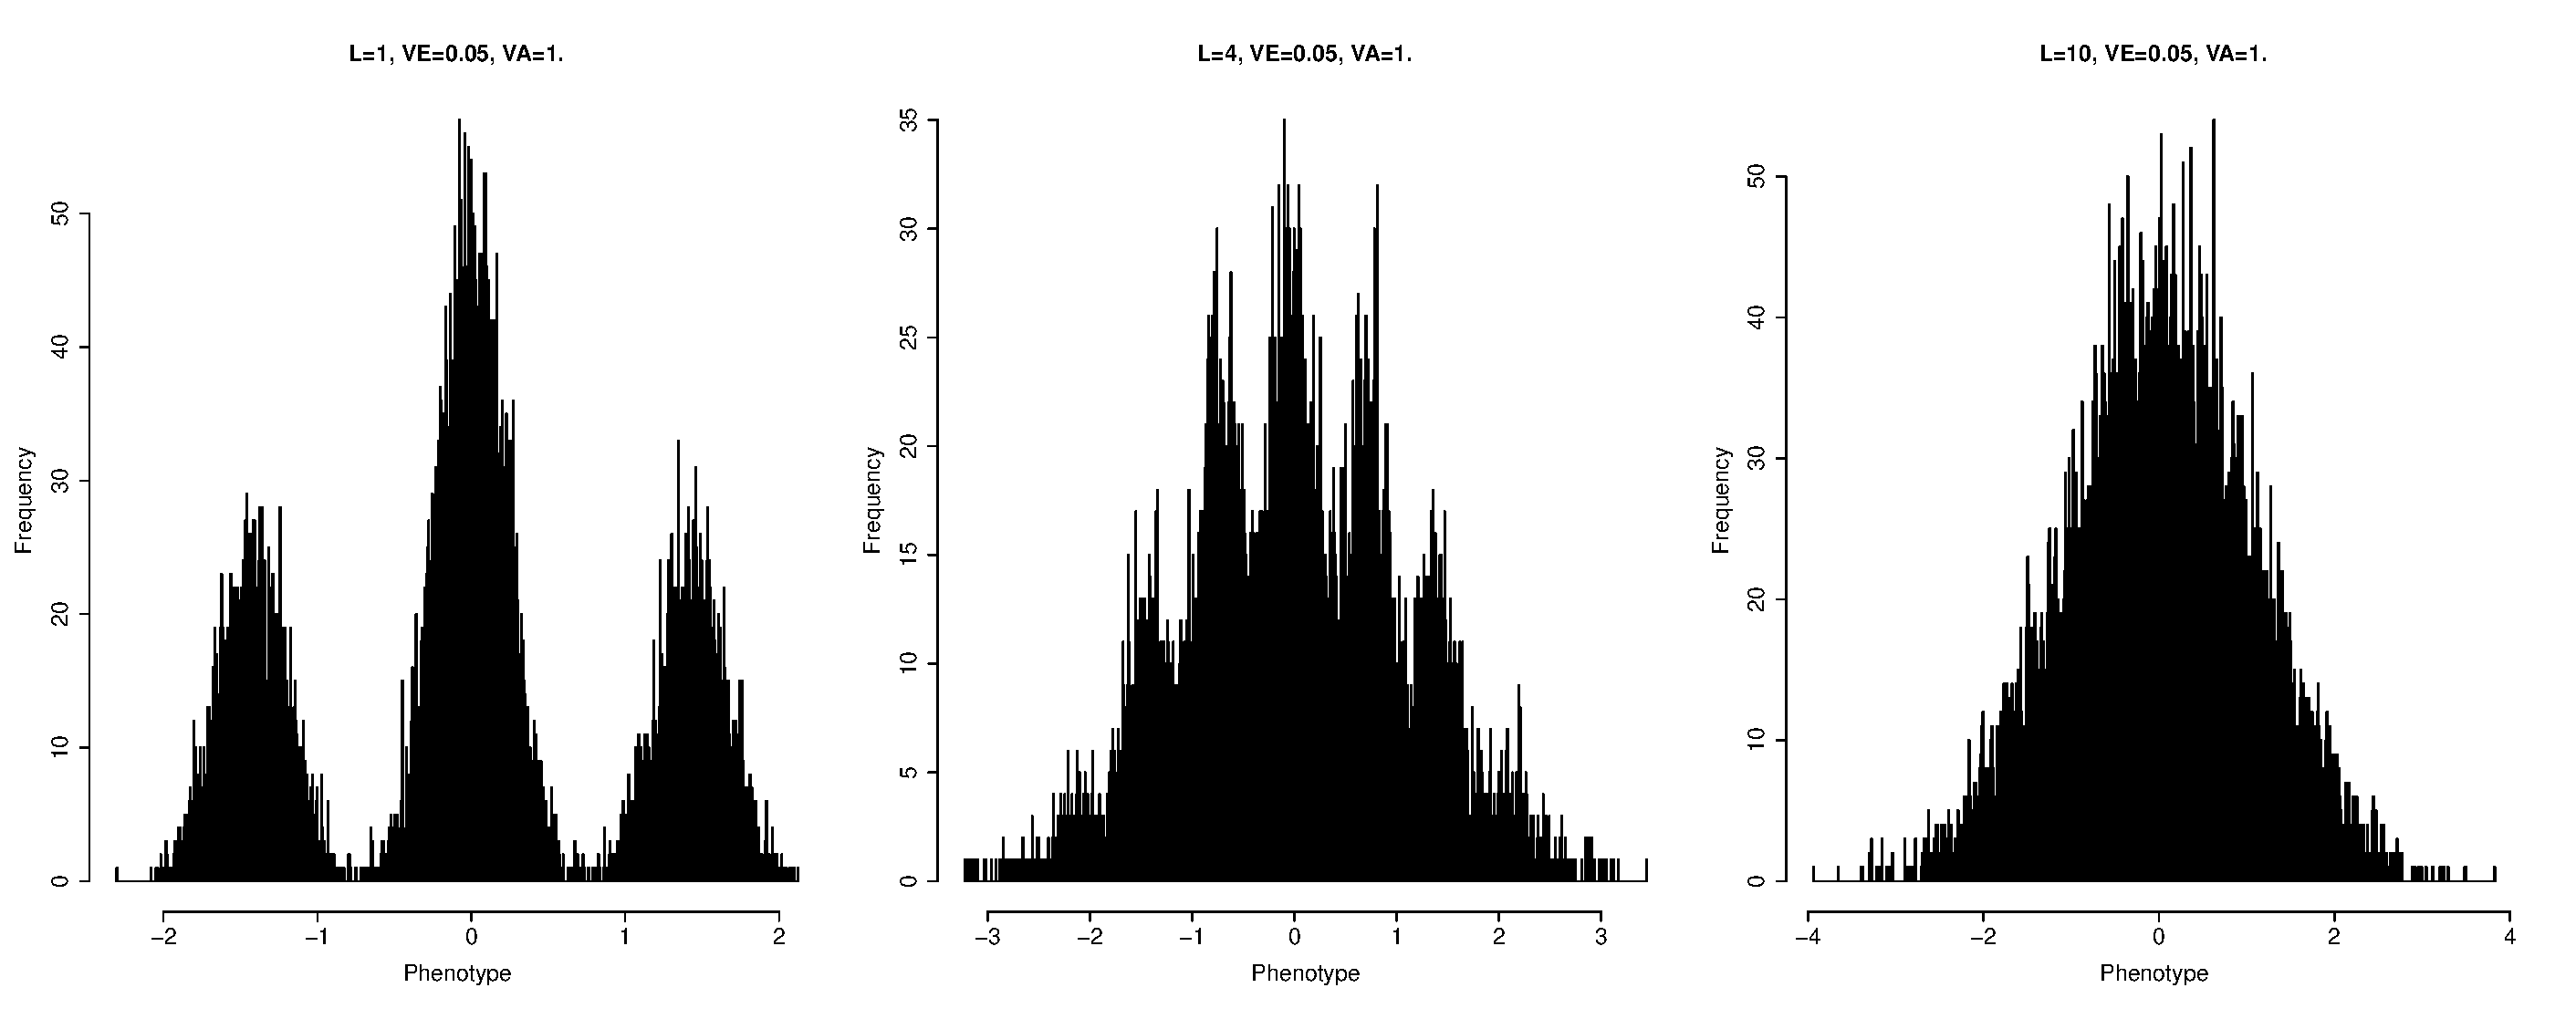
\includegraphics[width=0.8\textwidth]{Figs/QT1.eps}
\end{center}
\caption{The convergence of the phenotypic distribution to a normal distribution.} \label{fig:QT1}
\end{figure}

Note that as this is an additive model we can decompose eqn. \ref{pheno_geno_environ} into the
effects of the two alleles at each locus, in particular we can rewrite
it as
\begin{equation}
X_i = \mu + X_{iM}+X_{iP} +X_{iE}
\end{equation}
where $X_{iM}$ and $X_{iP}$ are the contribution to the phenotype of
the allele that our individual received from her mother (maternal
alleles) and father (paternal alleles) respectively. This will come in
handy in just a moment when we start thinking about the phenotype covariance of relatives.\\

Now obviously this model seems silly at first sight as alleles don't
only act in an additive manner, as they interact with alleles at the
same loci (dominance) and at different loci (epistasis). Later we'll
relax this assumption, 
however, we'll find that if we are interested in evolutionary change
over short time-scales it is actually only the ``additive
component'' of genetic variation that will (usually) concern us. 
We will define this more formally later on, but for the moment 
we can offer the intuition that parents only get to pass on a single
allele at each locus on to the next generation. As such, it is the
effect of these transmitted alleles, averaged over possible matings,
that is an individual's average contribution  to the next generation
(i.e. the additive effect of the alleles that their genotype consists of).


\subsubsection{Additive genetic variance and heritability}
As we are talking about an additive genetic model we'll talk about the
additive genetic variance ($V_A$), the variance due to the additive
effects of segregating genetic variation. This is a subset of the total genetic
variance if we allow for non-additive effects. \\

The variance of our phenotype across individuals ($V$) can write this as
\begin{equation}
V = Var(X_A) + Var(X_E) = V_A+V_E
\end{equation}
in writing this we are assuming that there is no covariance between $X_{G,i}$
and $X_{E,i}$ i.e. there is no covariance between genotype and
environment. \\

Our additive genetic variance can be written as
\begin{equation}
V_A = \sum_{l=1}^L Var(G_{i,l} a_{l})
\end{equation}
where $Var(G_{i,l} a_{l})$ is the contribution to the additive
variance among individuals of the $l$ locus. Assuming random mating we
can write our additive genetic variance as
\begin{equation}
V_A = \sum_{l=1}^L a_{l}^2 2 p_l(1-p_l)
\end{equation}
where the $ 2 p_l(1-p_l)$ term follows the binomial sampling of two
alleles per individual at each locus. \\

\paragraph{The narrow sense heritability}
We would like a way to think about what proportion of the variation
in our phenotype across individuals is due to genetic differences as
opposed to environmental differences. Such a quantity will be key in
helping us think about the evolution of phenotypes. For example, if
variation in our phenotype had no genetic basis then no matter how
much selection changes the mean phenotype within a generation
the trait will not change over generations. \\

We'll call the proportion of the variance that is genetic the
heritability, and denote it by $h^2$. We can then write this as
\begin{equation}
h^2 = \frac{Var(X_A)}{V} = \frac{V_A}{V}
\end{equation}
remember that we thinking about a trait where all of the alleles act
in a perfectly additive manner. In this case our heritability $h^2$ is
referred to as the narrow sense heritability, the proportion of the
variance explained by the additive effect of our loci.
When we allow dominance
and epistasis into our model we'll also have to define the broad sense
heritability (the total proportion of the phenotypic variance
attributable to genetic variation).\\

The narrow sense heritability of a trait is a useful quantity, indeed
we'll see shortly that it is exactly what we need to understand the
evolutionary response to selection on a quantitative phenotype. We can
calculate the narrow sense heritability by using the resemblance between
relatives. For example, if our phenotype was totally environmental we
should not expect relatives to resemble each other any more than random
individuals drawn from the population. Now the obvious caveat here is
that relatives also share an environment, so may resemble each other
due to shared environmental effects. \\

\subsubsection{The covariance between relatives}
So we'll go ahead and calculate the covariance in phenotype between two individuals
($1$ and $2$) who have a phenotype $X_1$ and $X_2$ respectively.
\begin{equation}
Cov(X_1,X_2) =
Cov\left((X_{1M}+X_{1P}+X_{1E}),((X_{2M}+X_{2P}+X_{2E}) \right)
\end{equation}
We can expand this out in terms of the covariance between the various
components in these sums.\\

To make our task easier we (and most analyses) will assume two things
\begin{enumerate}
\item that we can ignore the covariance of the environments
between individuals (i.e. $Cov(X_{1E},X_{2E})=0$)
\item that we can ignore the covariance
between the environment variation experience by an individual and the
genetic variation in another individual (i.e. $Cov(X_{1E},(X_{2M}+X_{2P}))=0$).
\end{enumerate}

The failure of these assumptions
to hold can severely undermine our estimates of heritability, but we'll
return to that later. Moving forward with these assumptions, we can
write our phenotypic covariance between our pair of individuals as
\begin{equation}
Cov(X_1,X_2) =
Cov((X_{1M},X_{2M})+Cov(X_{1M},X_{2P})+Cov(X_{1P},X_{2M})
+Cov(X_{1P},X_{2P}) \label{cov_rels_1}
\end{equation}
This is saying that under our simple additive model we can see the
covariance in phenotypes between individuals as the covariance between
the allelic effects in our individuals. We can use our results about
the sharing of alleles between relatives to obtain these terms.
But before we write down the general case lets quickly work through some
examples. \\


\paragraph{The covariance between Identical Twins}
Lets first consider the case of a pair of identical twins from two
unrelated parents. Our pair of twins share their maternal and paternal
allele identical by descent ($X_{1M}=X_{2M}$ and $X_{1P}=X_{2P}$). As their maternal and
paternal alleles are not correlated draws from the population,
i.e. have no probability of being $IBD$ as we've said the parents are unrelated, the
covariance between their effects on the phenotype is zero  
(i.e. $Cov(X_{1P},X_{2M})=Cov(X_{1M},X_{2P})=0$). In that case
eqn. \ref{cov_rels_1} is
\begin{equation}
Cov(X_1,X_2) = Cov((X_{1M},X_{2M})+Cov(X_{1P},X_{2P}) = 2Var(X_{1M})
= V_A
\end{equation}
Now in general identical twins are not going to be super helpful for
us in estimating $h^2$ as under models with non-additive effects
identical twins have higher covariance than we'd expect as they
resemble each other also because of the dominance effects as they
don't just share alleles they share their entire genotype.\\

\paragraph{The covariance in phenotype between mother and child}.
If the mother and father are unrelated individuals (i.e. are two
random draws from the population) then the mother and a child share
one allele IBD at each locus (i.e. $r_1=1$ and $r_0=r_2=0$). Half the
time our mother transmits her paternal allele to the child, in which
case $X_{P1}=X_{M2}$ and so $Cov(X_{P1},X_{M2})=Var(X_{P1})$ and all
the other covariances in eqn. \ref{cov_rels_1} zero, and half
the time she transmits her maternal allele to the child
$Cov(X_{M1},X_{M2})=Var(X_{M1})$ and all the other terms zero. By this
argument $Cov(X_1,X_2) = \half Var(X_{M1}) + \half Var(X_{P1}) = \half
V_A$. \\

\paragraph{The covariance between general pairs of relatives under an
additive model}
The two examples make clear that to understand the covariance between
phenotypes of relatives we simply need to think about the alleles they
share IBD. Consider a pair of relatives ($1$ and $1$) with a probability $r_0$,
$r_1$, and $r_2$ of sharing zero, one, or two alleles IBD
respectively. When they share zero alleles
$Cov((X_{1M}+X_{1P}),(X_{2M}+X_{2P}))=0$, when they share one allele
$Cov((X_{1M}+X_{1P}),(X_{2M}+X_{2P}))=
Var(X_{1M})=\frac{1}{2}V_A$, and when they share two alleles $Cov((X_{1M}+X_{1P}),(X_{2M}+X_{2P}))=
V_A$. Therefore, the general covariance between two
relatives is
\begin{equation}
Cov(X_1,X_2) = r_0 \times 0 + r_1 \frac{1}{2}V_A + r_2  V_A =
2 F_{1,2} V_A
\end{equation}\\
So under a simple additive model of the genetic basis of a phenotype
to measure the narrow sense heritability we need to measure the
covariance between a set of pairs of relatives (assuming that we can remove the effect of
shared environmental noise). From the covariance between relatives we
can calculate $V_A$, we can then divide this by the total phenotypic
variance to get $h^2$. \\
%One way potentially to get somewhat around the
%shared environmental effect is to use paternal half-sibs as they share a

Another way that we can estimate the narrow sense heritability is
through the regression of child's phenotype on the parental mid-point
phenotype. The parental mid-point phenotype is simple the average of
the mum and dad's phenotype. Denoting the child's phenotype by $X_{kid}$ and mid-point
phenotype by $X_{mid}$ so that if we take the regression $X_{kid} \sim X_{mid}$ this
regression has slope $\beta = Cov(X_{kid},X_{mid})/Var(X_{mid})$.
The covariance of $Cov(X_{kid},X_{mid})=\half
V_A$, and $Var(X_{mid}) = \half V$ as by taking the average of the
parents we have halved the variance, such that the slope of the
regression is
\begin{equation}
\beta= \frac{Cov(X_{kid},X_{mid})}{Var(X_{mid})} = \frac{V_A}{V} = h^2
\end{equation}
i.e. the regression of the child's phenotype on the parental midpoint
phenotype is an estimate of the narrow sense heritability. This is a
common way to estimate heritability, although it doesn't bypass the
need to control for environmental correlations between relatives. \\

Our regression allows us to attempt to predict the phenotype of the
child given the child; how well we can do this depends on the
slope. If the slope is close to zero then the parental phenotypes hold no
information about the phenotype of the child, while if the slope is
close to one then the parental mid-point is a good guess at the child's
phenotype.\\
\begin{figure}
\begin{center}
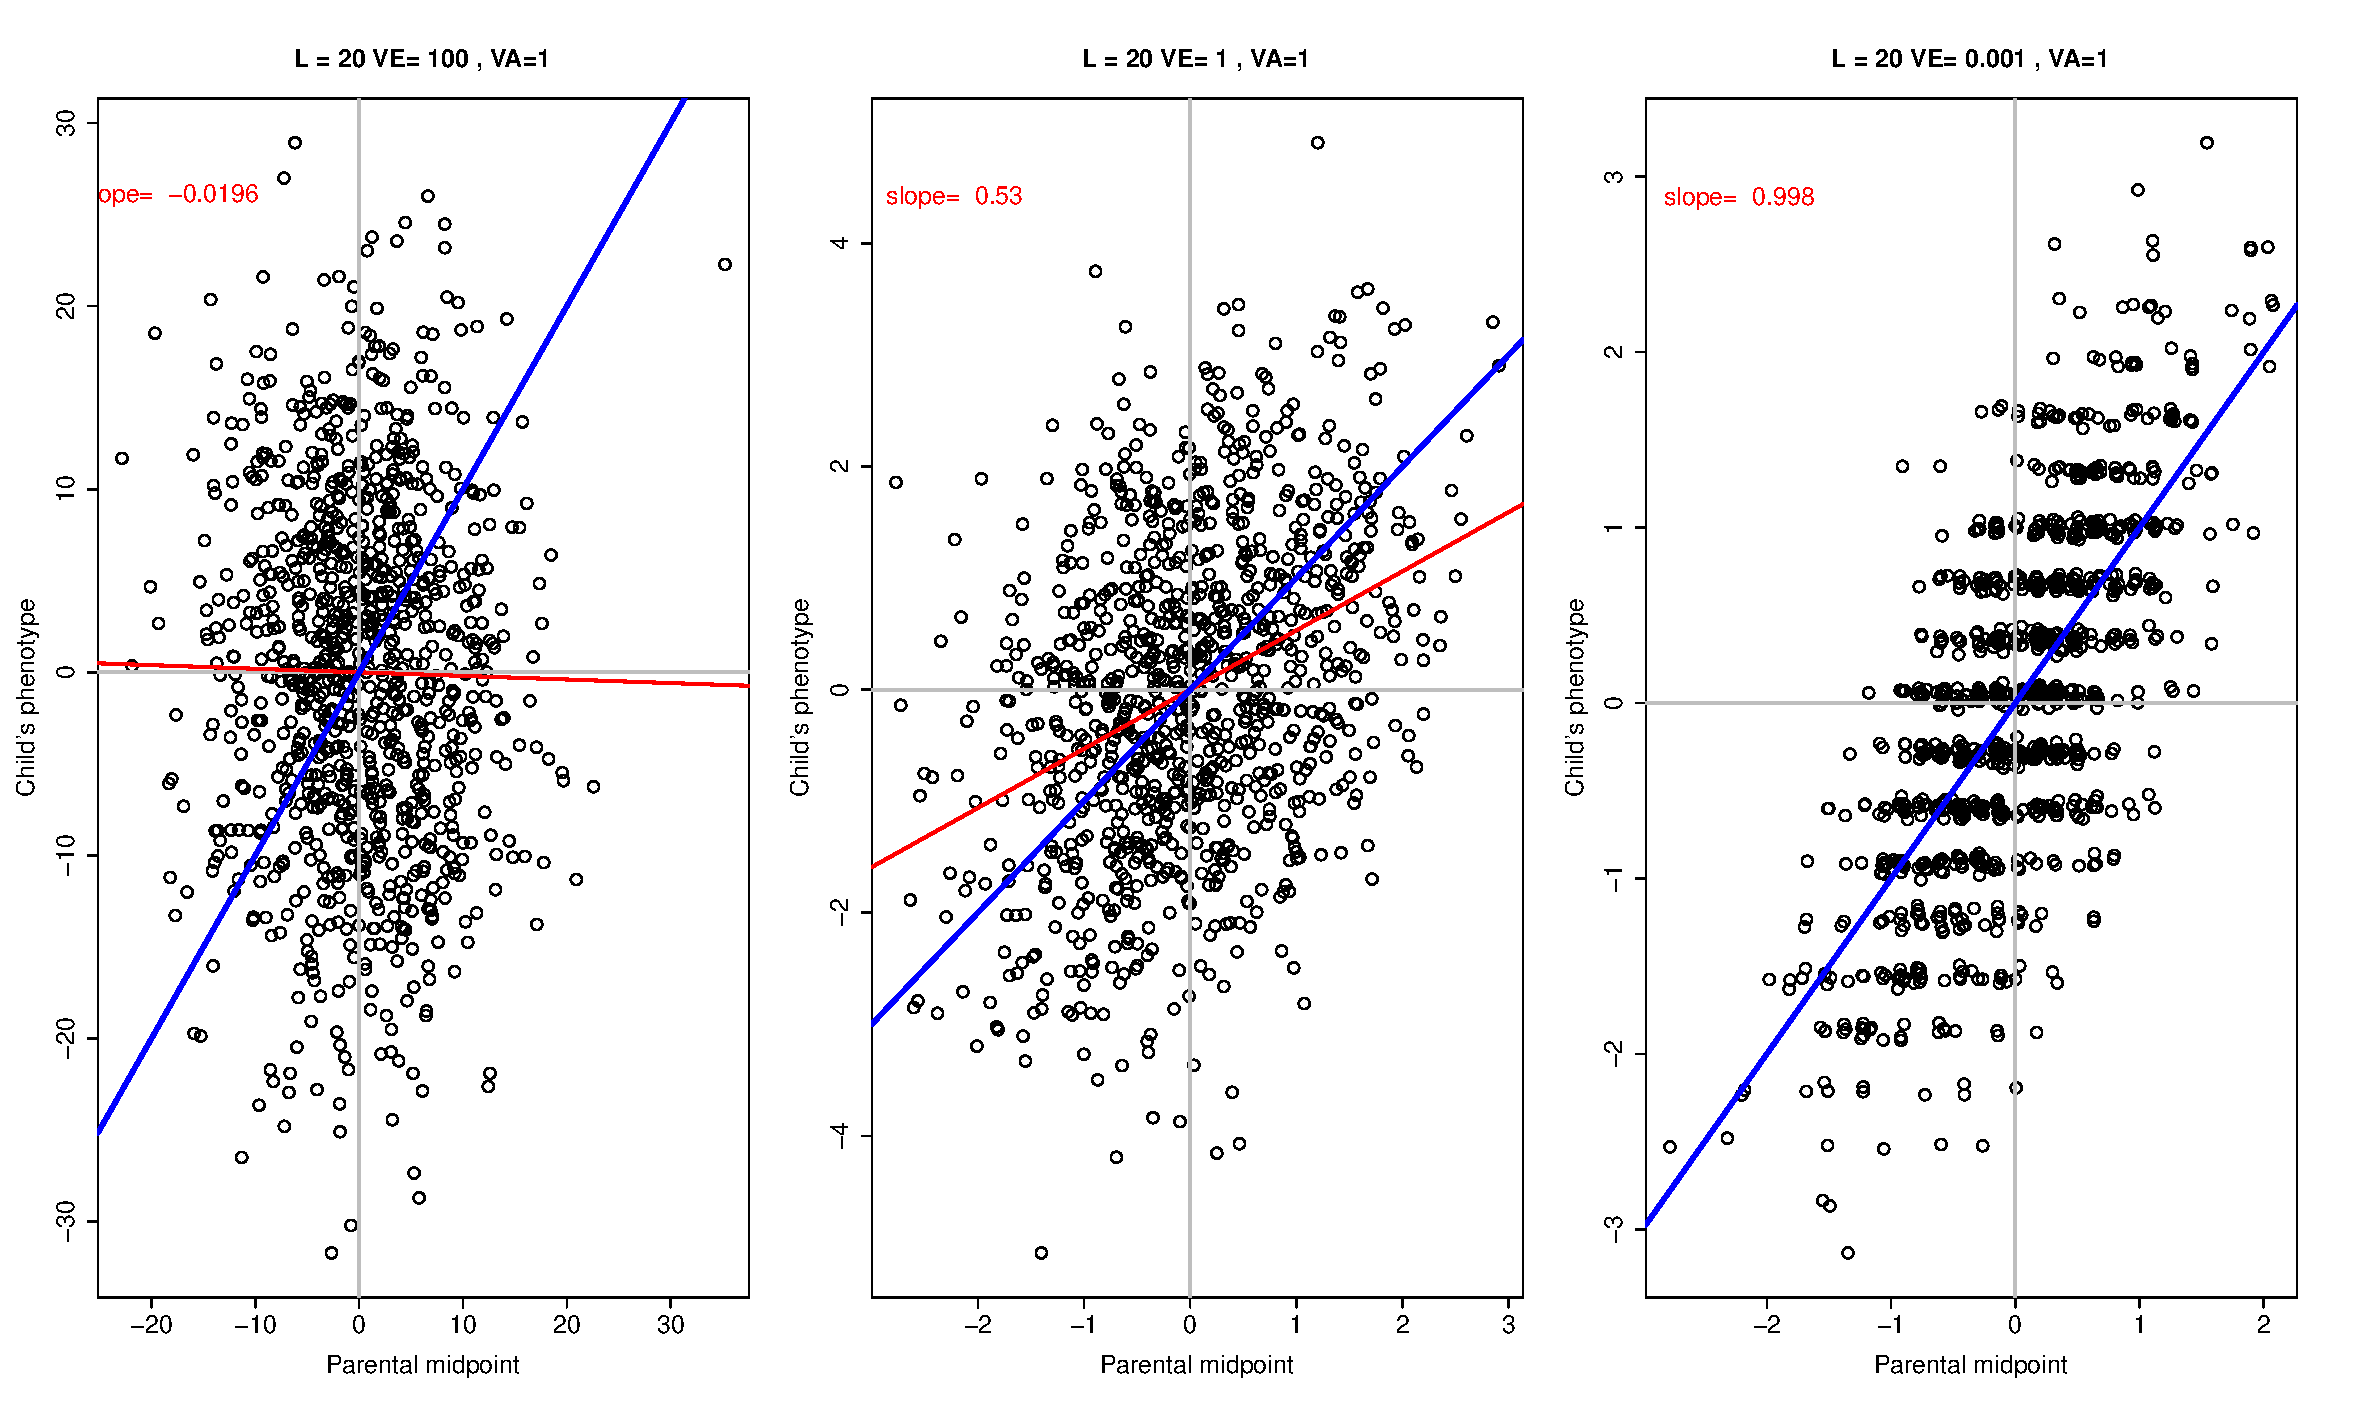
\includegraphics[width=0.8\textwidth]{Figs/QT2.eps}
\end{center}
\caption{Regression of parental mid-point phenotype on child's
  phenotype.}
\end{figure}

More formally the expected phenotype of the child given the parental
phenotypes is
\begin{equation}
\E(X_{kid} | X_{mum},X_{dad}) = \mu +
\beta(X_{mid} - \mu) =\mu + h^2(X_{mid} - \mu)  \label{predict_kid}
\end{equation}
this follows from the definition of linear regression. So to find the
child's predicted phenotype we simply take the mean phenotype and add
on the difference between our parental mid-point multiplied by our
narrow sense heritability. \\


\paragraph{Estimating additive genetic variance across a variety of
  different relationships.}

In many natural populations we may have access to individuals of a
range of different relationships to each other (through monitoring
of the paternity of individuals), but relatively few individuals of a
given relationship (e.g. sibs). We can try and use this information as
fully as possible in a mixed model framework. Considering equation
\ref{pheno_geno_environ} we can write an individual's phenotype $X_i$
 as 
\begin{equation}
X_i =  \mu  + X_{A,i} + e_i 
\end{equation}
where $e_i \sim N(0,V_E)$ and $X_{A,i}$ is normally distributed across
individuals with covariance matrix $V_A A$ where the the entries for
an pair of individuals i and i are 
$A_{ij}= 2 F_{i,j}$ and $A_{ii} 1$. Given the matrix $A$ we can estimate $V_A$. We can
also add fixed effects into this model to account for generation
effects, additional mixed effects could also be included to account
for shared environments between particular individuals (e.g. a shared nest).
This is sometimes called the ``animal model'', and also goes by the
name of variance components analysis.

\paragraph{Multiple traits.}

Traits often covary with each other, due to both environmentally
induced effects (e.g. due to the effects of diet on multiple traits)
and due to the expression of underlying genetic covariance between
traits. In turn this genetic covariance can reflect pleiotropy, a
mechanistic effect of an allele on multiple traits (e.g. variants that
effect skin pigmentation often effect hair color) or the genetic
linkage of loci independently affecting multiple traits. If we are
interested in evolution over short time-scales we can (often) ignore
the genetic basis of this correlation. 

Consider two traits $X_{1,i}$ and $X_{2,i}$ in an indivdual $i$, these could be
say the indivdual's leg length and nose length. As before we can write
these as 
\begin{eqnarray}
X_{1,i} &= \mu_1+ X_{1,A,i} + X_{1,E,i}  \nonumber \\
X_{2,i} &= \mu_2 +X_{2,A,i} + X_{2,E,i} \nonumber \\
\end{eqnarray}
As before we can talk about the total phenotypic variance ($V_1,V_2$),
environmental variance  ($V_{1,E}$ and $V_{2,E}$), and the additive variance and in trait one and two
and ($V_{1,A}$, $V_{2,A}$). But now we also have to consider the 
total covariance $V_{1,2}=Cov(X_{1},X_{2})$, the environmentally induced covariance between the traits ($V_{E,1,2}=Cov(X_{1,E}
,X_{2,E} )$) and the additive genetic covariance ($V_{A,1,2}
=Cov(X_{1,A} ,X_{2,A} )$) between trait one and two.

We can store these values in a matrices 
\begin{equation}
\bf{V}= \left( \begin{array}{cc} 
V_{1} & V_{1,2} \\
V_{1,2} & V_{2} \\
\end{array} \right) \label{P_matrix}
\end{equation}
and
\begin{equation}
\bf{G}= \left( \begin{array}{cc} 
V_{1,A} & V_{A,1,2} \\
V_{A,1,2} & V_{2,A} \\
\end{array} \right)  \label{G_matrix}
\end{equation}
we can generalize this to an abitrary number of traits.

We can estimate these quantities, in a similar way to before, by
studying the covariance in different traits between relatives: 

\begin{equation}
Cov(X_{1,i},X_{2,j}) = 2 F_{i,j} V_{A,1,2}
\end{equation}



\subsubsection{The response to selection}
Evolution by natural selection requires:
\begin{enumerate}
\item Variation in a phenotype
\item That survival is non-random with respect to this phenotypic
variation.
\item That this variation is heritable.
\end{enumerate}
Points 1 and 2 encapsulate our idea of Natural Selection, but evolution by natural
selection will only occur if the 3rd condition is met. It is the
heritable nature of variation that couples change within a generation
due to natural selection, to change across generations (evolutionary
change). \\

Lets start by thinking about the change within a generation due
to directional selection, where selection acts to change the mean
phenotype within a generation. For example, a decrease in mean height within a
generation, due to taller organisms having a lower chance of surviving
to reproduction than shorter organisms. Specifically, we'll denote our mean phenotype at
reproduction by $\mu_S$, i.e. after selection has acted, and our mean
phenotype before selection acts by $\mu_{BS}$. This second quantity may be hard to
measure, as obviously selection acts throughout the life-cycle, so it
might be easier to think of this as the mean phenotype if selection
hadn't acted. So the mean phenotype changes within a generation is $\mu_{S} - \mu_{BS}= S$.  \\

We are interested in predicting the distribution of phenotypes in next
generation, in particular we are interested in the mean phenotype in
the next generation to understand how directional selection has
contributed to evolutionary change. We'll denote the mean phenotype in
offspring, i.e. the mean phenotype in the next generation before selection acts,
as $\mu_{NG}$. The change across generations we'll call the response
to selection $R$ and put this equal to $\mu_{NG}- \mu_{BS}$. \\

The mean phenotype in the next generation is
\begin{equation}
\mu_{NG} = \E \left( \E(X_{kid} | X_{mum},X_{dad}) \right)
\end{equation}
where the outer expectation is over the randomly mating of individuals
who survive to reproduce. We can use eqn. \ref{predict_kid} to obtain
an expression for this
\begin{equation}
\mu_{NG} = \mu_{BS} +
\beta ( \E(X_{mid}) - \mu_{BS})
\end{equation}
so to obtain $\mu_{NG}$ we need to compute $\E(X_{mid})$ the expected
mid-point phenotype of pairs of individuals who survive to
reproduce. Well this is just the expected phenotype in the individuals
who survived to reproduce ($\mu_{S}$), so
\begin{equation}
\mu_{NG} = \mu_{BS} +
h^2 (\mu_S - \mu_{BS})
\end{equation}
So we can write our response to selection as
\begin{equation}
R = \mu_{NG} -\mu_{BS}  =
h^2 (\mu_S - \mu_{BS}) = h^2 S \label{breeders_eqn}
\end{equation}
So our response to selection is proportional to our selection
differential, and the constant of proportionality is the narrow sense
heritability. This equation is sometimes termed the Breeders
equation. It is a statement that the evolutionary change across
generations ($R$) is proportional to the change caused by directional selection
within a generation, and the strength of this relationship is
determined by the narrow sense heritability. \\

Using the fact that $h^2=V_A/V$ we can rewrite this in a different form as
\begin{equation}
R= V_A \frac{S}{V}
\end{equation}
i.e. our response to selection is the additive genetic variance of our
trait ($V_A$) multiplied by the change within a generation as a
fraction of the total phenotypic variance ($S/V$, sometimes called the
the selection gradient $\beta$).\\


\begin{figure}
\begin{center}
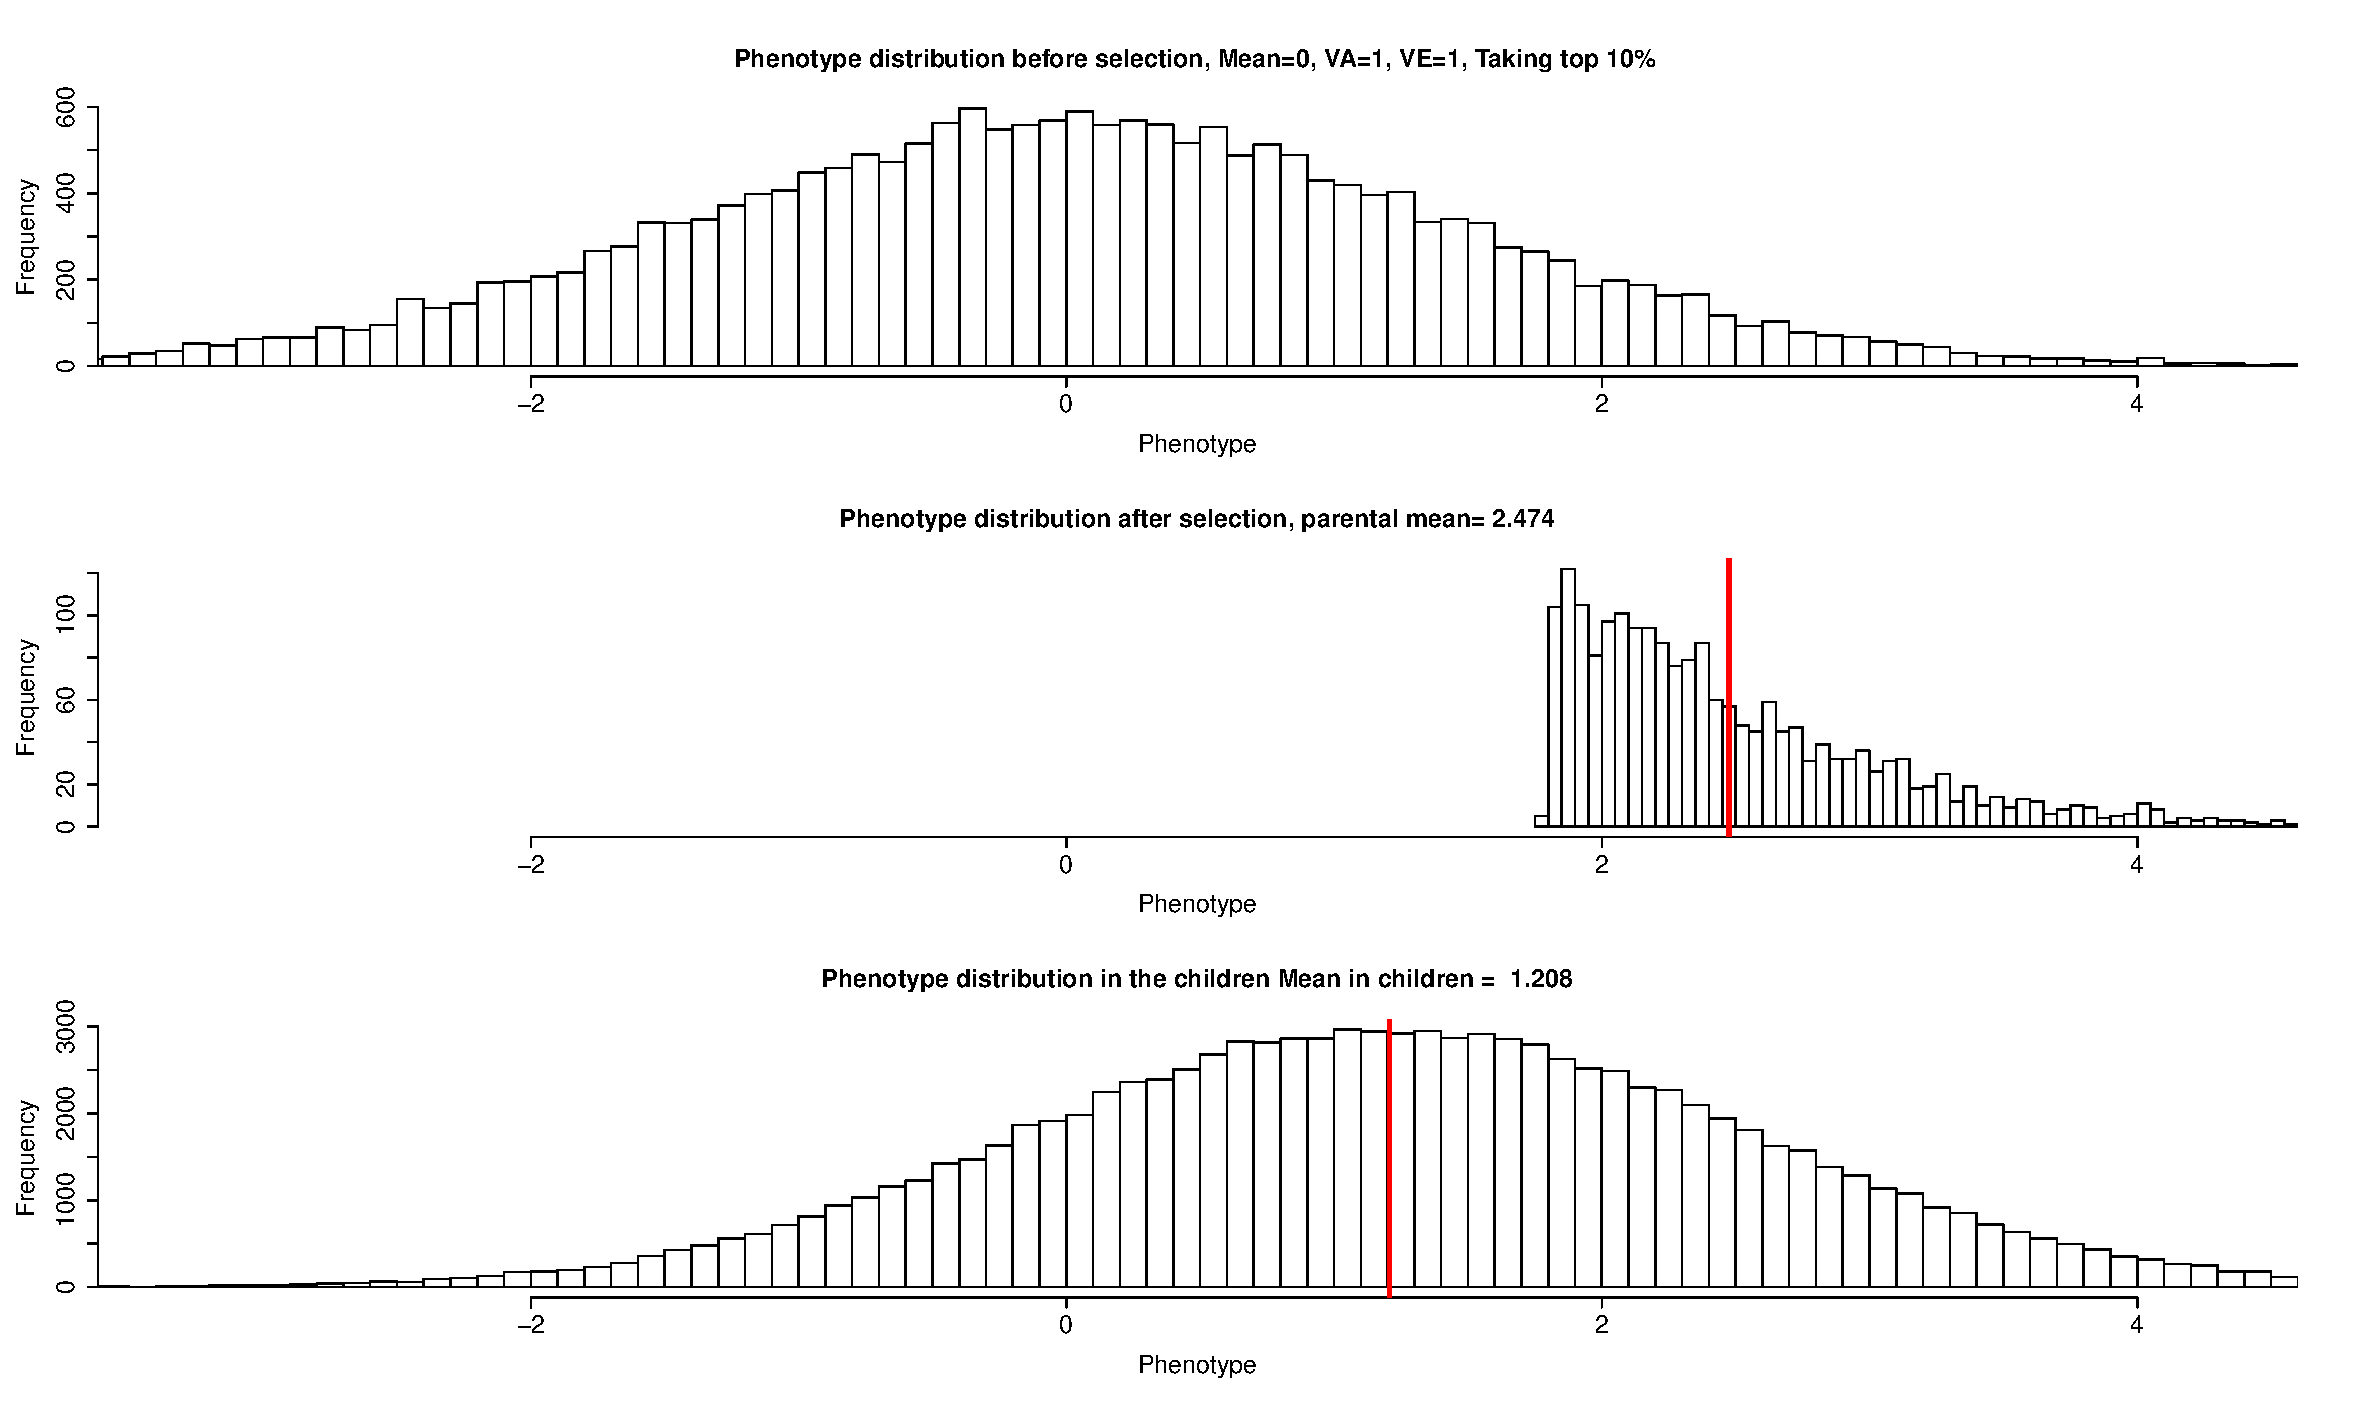
\includegraphics[width=0.8\textwidth]{Figs/QT3.eps}
\end{center}
\end{figure}

A change in mean phenotype within a generation occurs because of the
differential fitness of our organisms. To think more carefully about this change within a
generation lets think about a simple fitness model where our phenotype affects the
viability of our organisms (i.e. the probability they survive to
reproduce). The probability that an individual has a phenotype $X$
before selection is $p(X)$, so that the mean phenotype before
selection is
\begin{equation}
\mu_{BS} = \E[X] =  \int_{-\infty}^{\infty} x p(x) dx
\end{equation}
The probability that an organism with a phenotype $X$ survives to
reproduce is $w(X)$, and we'll think about this as the fitness of
our organism. The probability distribution of phenotypes in those who
do reproduce is
\begin{equation}
\P(X | \textrm{survive}) =  \frac{p(x) w(x)}{
\int_{-\infty}^{\infty} p(x) w(x) dx}.
\end{equation}
where the denominator is a normalization constant which ensures that
our phenotypic distribution integrates to one. The denominator also
has the interpretation of being the mean fitness of the population,
which we'll call $\wbar$, i.e.  
\begin{equation}
\wbar =  
\int_{-\infty}^{\infty} p(x) w(x) dx.
\end{equation}

Therefore, we can write the mean phenotype in those who survive to
reproduce as
\begin{equation}
\mu_S = \frac{1}{\wbar}\int_{-\infty}^{\infty} x p(x) w(x) dx
\end{equation}

If we mean center our population, i.e. set the phenotype before
selection to zero, then
\begin{equation}
S= \frac{1}{\wbar}\int_{-\infty}^{\infty} x p(x) w(x) dx
\end{equation}
if $\mu_S=0$.  Inspecting this more closely we can see that $S$ has
the form of a covariance between our phenotype $X$ and our fitness
$w(X)$ ($Cov(X,w(X))$). Thus our change in mean phenotype is directly a measure of the
covariance of our phenotype and our fitness. Rewriting our breeder's
equation using this observation we see
\begin{equation}
R = \frac{V_A}{V}  Cov(X,w(X))
\end{equation}
we see that the response to selection is due to the fact that our
fitness (viability) of our organisms/parents covaries with our phenotype, and
that our child's phenotype is correlated with the parent phenotype.

\paragraph{The response of multiple traits to selection, the
  multivariate breeder's equation.}
We can generalize these results for multiple traits, to ask how selection on
multiple phenotypes plays out over short time intervals. We'll write
our change in the mean our multiple phenotypes within a generation as
the vector $\bf{S}$ and our response across multiple generations as
the vector $\bf{R}$. These two quantities are related by 
\begin{equation}
\bf{R} = \bf{G} \bf{V}^{-1} \bf{S} = \bf{G} \bf{\beta}
\end{equation}
 where $\bf{V}$ and $\bf{G}$ are our matrices of the
 variance-covariance of phenotypes and additive genetic values
 (eqn. \eqref{G_matrix} \eqref{P_matrix}) and
 $\bf{\beta}$ is a vector of selection gradients (i.e. the change
 within a generation as a fraction of the total phenotypic variance).
To make this a bit more intuitive, consider two traits we are writing 
\begin{eqnarray}
R_1 & = V_{A,1} \beta_1 + V_{A,1,2} \beta_2 \nonumber \\
R_2 & = V_{A,2} \beta_2 + V_{A,1,2} \beta_1  \nonumber \\
\end{eqnarray}
where the $1$ and $2$ index our two different traits. This is a
statement that our response in any one phenotype is modified by
selection on other traits that covary with that trait.
This offers a good way to think about how genetic trade offs play out
over evolution over short time-scales.



\newpage
\section{One-locus models of selection}

\subsection{Fitness}

As we have seen, natural selection occurs when there are differences between individuals in fitness. We may define fitness in various ways. Most commonly, it is defined with respect to the contribution of a phenotype or genotype to the next generation. 
Differences in fitness can arise at any point during the life cycle. For instance, different genotypes or phenotypes may have different survival probabilities from one stage in their life to the stage of reproduction (viability), or they may differ in the number of offspring produced (fertility), or both. Here, we define the absolute fitness of a genotype as the expected number of offspring of an individual of that genotype. \\

\subsection{Haploid selection model}
We start out by modelling selection in a haploid model, as this is mathematically relatively simple. Let the number of individuals carrying alleles $A_1$ and $A_2$ in generation $t$ be $P_t$ and $Q_t$. Then, the relative frequencies at time $t$ of alleles $A_1$ and $A_2$ are $p_t = P_t / (P_t + Q_t)$ and $q_t = Q_t / (P_t + Q_t) = 1 - p_t$. Further, assume that individuals of type $A_1$ and $A_2$ on average produce $W_1$ and $W_2$ offspring individuals, respectively. We call $W_i$ the absolute fitness.\\

Therefore, in the next generation, the absolute number of carriers of $A_1$ and $A_2$ are $P_{t+1} = W_1 P_t$ and $Q_{t+1} = W_2 Q_t$, respectively. The mean absolute fitness of the population at time $t$ is
\begin{equation}
	\label{eq:meanAbsFit}
	\Wbar_t = W_1 \frac{P_t}{P_t + Q_t} + W_2 \frac{Q_t}{P_t + Q_t} = W_1 p_t + W_2 q_t,	
\end{equation}
i.e.\ the sum of the fitness of the two types weighted by their
relative frequencies. Note that the mean fitness depends on time, as
it is a function of the allele frequencies, which are themselves time
dependent. \\

The frequency of allele $A_1$ in the next generation is then given by
\begin{equation}
	\label{eq:eq:recHaplMod1}
	p_{t+1} = \frac{P_{t+1}}{P_{t+1} + Q_{t+1}} = \frac{W_1 P_t}{W_1 P_t + W_2 Q_t}
	%= \frac{W_1 (P_t + Q_t)p_t}{W_1 (P_t + Q_t)p_t + W_2 (P_t + Q_t)q_t}
	= \frac{W_1 p_t}{W_1 p_t + W_2 q_t} = \frac{W_1}{\Wbar_t} p_t.
\end{equation}


Importantly, eqn.\ (\ref{eq:eq:recHaplMod1}) tells us that the change in $p$ only depends on a ratio of fitnesses. Therefore, we need to specify fitness only up to an arbitrary constant. As long as we multiply all fitnesses by the same value, that constant will cancel out and eqn.\ (\ref{eq:eq:recHaplMod1}) will hold. Based on this argument, it is very common to scale absolute fitnesses by the absolute fitness of one of the genotypes, e.g.\ the most or the least fit genotype, to obtain relative fitnesses. Here, we will use $w_i$ for the relative fitness of genotype $i$. If we choose to scale by the absolute fitness of genotype $A_1$, we obtain the relative fitnesses $w_1 = W_1/W_1 = 1$ and $w_2 = W_2/W_1$.\\
Without loss of generality, we can therefore rewrite eqn.\ (\ref{eq:eq:recHaplMod1}) as
\begin{equation}
	\label{eq:recHaplMod2}
	p_{t+1} = \frac{w_1}{\wbar} p_t,
\end{equation}
dropping the dependence of the mean fitness on time in our notation, but remembering it.
The change in frequency from one generation to the next is then given by
\begin{equation}
\Delta p_t = p_{t+1} - p_t= \frac{ w_1 p_t}{ \wbar} - p_t = \frac{w_1 p_t - \wbar p_t}{\wbar} = \frac{w_1 p_t - (w_1 p_t + w_2 q_t) p_t}{\wbar} = \frac{w_1 - w_2}{\wbar} p_t q_t,
\label{eq:deltap_haploid}
\end{equation}
recalling that $q_t = 1 - p_t$.\\

Assuming that the fitnesses of the two alleles are constant over time,
the number of the two allelic types $\tau$ generations after time $t$ are
$P_{t+\tau} = (W_1)^{\tau} P_t$ and $Q_{t+\tau}=  (W_2)^{\tau} Q_t$, respectively. Therefore, the relative frequency of allele $A_1$ after $\tau$ generations past $t$ is
\begin{equation}
	p_{t+\tau} = \frac{ (W_1)^{\tau} P_t}{ (W_1)^{\tau} P_t+(W_2)^{\tau} Q_t} = \frac{ (w_1)^{\tau} P_t}{ (w_1)^{\tau} P_t+(w_2)^{\tau} Q_t} = \frac{p_t}{p_t + (w_2/w_1)^{\tau} q_t},
	\label{eq:haploid_tau_gen}
\end{equation}
where the last step includes dividing the whole term by $w_1$ and switching from absolute to relative allele frequencies.\\

Rearranging eqn.\ \eqref{eq:haploid_tau_gen} and setting $t = 0$, we can work out the time $\tau$ for the frequency of $A_1$ to change from $p_0$ to $p_{\tau}$. First, we write
\begin{equation}
	p_{\tau} = \frac{p_0}{p_0 + (w_2/w_1)^{\tau} q_0}
\end{equation}
and rearrange this to obtain
\begin{equation}
	\label{eq:estTau}
	\frac{p_{\tau}}{q_{\tau}} = \frac{p_0}{q_0} \left(\frac{w_1}{w_2}\right)^{\tau}.
\end{equation}
Solving this for $\tau$ yields
\begin{equation}
	\label{eq:solTau}
	\tau = \log \left(\frac{p_{\tau} q_0}{q_{\tau} p_0}\right) /  \log\left(  \frac{w_1}{w_2} \right).
\end{equation}
\\

In practice, it is often helpful to parametrize the relative fitnesses $w_i$ in a specific way. For example, we may set $w_1 = 1$ and $w_2 = 1 - s$, where $s$ is called the selection coefficient. Using this parametrization, $s$ is simply the difference in relative fitnesses between the two alleles. Equation \eqref{eq:haploid_tau_gen} becomes
\begin{equation}
	\label{eq:haploid_tau_gen_expl}
	p_{t+\tau} = \frac{p_{t}}{p_{t} + q_{t} (1 - s)^{\tau}},
\end{equation}
as $w_2 / w_1 = 1 - s$. Then, if $s \ll 1$, we can approximate $(1-s)^{\tau}$ in the denominator by $\exp(-s\tau)$ to obtain
\begin{equation} \label{eq:haploid_logistic growth}
	p_{t+\tau} \approx \frac{p_t}{p_t + q_t e^{-s\tau}}.
\end{equation}
This equation takes the form of a logistic function. That is because
we are looking at the relative frequencies of two `populations' (of
alleles $A_1$ and $A_2$) that are growing (or declining)
exponentially, under the constraint that $p$ and $q$ always sum to 1. \\

Moreover, eqn.\ \eqref{eq:estTau} for the time $\tau$ it takes for a certain change in frequency to occur becomes
\begin{equation}
	\label{eq:estTauExpl}
	\tau = - \log \left(\frac{p_{\tau} q_0}{q_{\tau} p_0}\right) /  \log\left(1-s\right).
\end{equation}
Assuming again that $s \ll 1$, this simplifies to
\begin{equation}
	\label{eq:estTauExplSimpl}
	\tau \approx \frac{1}{s} \log \left(\frac{p_{\tau} q_0}{q_{\tau} p_0}\right).
\end{equation}


One particular case of interest is the time it takes to go from an absolute frequency of 1 to near fixation in a population of size $N$. In this case, we have $p_0 = 1/N$, and we may set $p_{\tau} = 1 - 1/N$, which is very close to fixation. Of course, we then have $q_0 = 1 - 1/N$ and $q_{\tau} = 1 - 1/N$. If $N$ is sufficiently large, we may for mathematical convenience approximate $q_0$ by $q_0 = 1$. Plugging these values into eqn.\ \eqref{eq:estTauExplSimpl}, we obtain
\begin{equation}
	\label{eq:fixTimeSimpl}
	\tau \approx \frac{1}{s} \log\left( \frac{1 - 1/N}{(1 - 1/N)\ 1/N}  \right) = \frac{1}{s} \log(N)
\end{equation}
as an approximation for the time to fixation.


\paragraph{Haploid model with fluctuating selection}
We can now consider the case where the fitnesses depend on time, and
say that $w_{1,t}$ and $w_{2,t}$ are the fitnesses of the two types in
generation $t$. The frequency of allele $A_1$ in generation $t+1$ is
\begin{equation}
p_{t+1} = \frac{w_{1,t}}{\wbar_t} p_t,
\end{equation}
which simply follows from eqn.\ \eqref{eq:recHaplMod2}.
The ratio of the frequency of allele $A_1$ to that of allele $A_2$ in generation $t+1$ is
\begin{equation}
\frac{p_{t+1}}{q_{t+1}} = \frac{w_{1,t}}{w_{2,t}}  \frac{p_{t}}{q_{t}}.
\end{equation}
Therefore, if we think of the two alleles starting in generation $t$ at
frequencies $p_t$ and $q_t$, then $\tau$ generations later,
\begin{equation}
\frac{p_{t+\tau}}{q_{t+\tau}} = \left(\prod_{i=t}^{\tau-1} \frac{w_{1,i}}{w_{2,i}}  \right) \frac{p_{t}}{q_{t}}.
\end{equation}
\\

The question of which allele is increasing or decreasing in frequency comes down
to whether $\left(\prod_{i=t}^{\tau-1} \frac{w_{1,i}}{w_{2,i}}  \right)$ is
$>1$ or $<1$. As it is a little hard to think about this ratio, we can
instead take the $\tau^{\mathrm{th}}$ root of it and consider
\begin{equation}
\sqrt[\tau]{\left(\prod_{i=t}^{\tau-1} \frac{w_{1,i}}{w_{2,i}}  \right)} = \frac{\sqrt[\tau]{\prod_{i=t}^{\tau-1}w_{1,i}}}{\sqrt[\tau]{\prod_{i=t}^{\tau-1}w_{2,i}}}.
\end{equation}
The term $\sqrt[\tau]{\prod_{i=t}^{\tau-1}w_{1,i}}$ is the geometric mean fitness of allele
 $A_1$ over the $\tau$ generations past generation $t$. Therefore, allele $A_1$ will only increase
in frequency if it has a higher geometric mean fitness than allele $A_2$
(at least in our simple deterministic model). \\


\subsection{Diploid model}
We will now move on to a diploid model of a single locus with two segregating alleles.
We will assume that the difference in fitness between the three
genotypes comes from differences in viability, i.e.\ differential
survival of individuals from the formation of zygotes to reproduction.  
We denote the absolute fitnesses of genotypes $A_1A_1$, $A_1A_2$, and $A_2A_2$ by $W_{11}$, $W_{12}$, and $W_{22}$. Specifically, $W_{ij}$ is the probability that a zygote of genotype $A_iA_j$ survives to reproduction.
Assuming that individuals mate at random, the number of zygotes that are of the three genotypes and form generation $t$ are
\begin{equation}
Np_t^2, ~~~  N2p_tq_t, ~~~ Nq_t^2.
\end{equation}

The mean fitness of the population of zygotes is then
\begin{equation}
	\Wbar_t = W_{11} p_t^2+W_{12} 2p_tq_t  +  W_{22} q_t^2.
\end{equation}
Again, this is simply the weighted mean of the genotypic fitnesses.
\\

How many zygotes of each of the three genotypes survive to reproduce?
An individual of genotype $A_1A_1$ has a probability of $W_{11}$ of
surviving to reproduce, and similarly for other genotypes. Therefore, the expected number of $A_1A_1$, $A_1A_2$, and $A_2A_2$ individuals who survive to reproduce is
\begin{equation}
	NW_{11} p_t^2, ~~~ NW_{12} 2p_tq_t , ~~~ N W_{22} q_t^2.
\end{equation}
It then follows that the total number of individuals who survive to
reproduce is
\begin{equation}
	N \left(W_{11} p_t^2+W_{12} 2p_tq_t  +  W_{22} q_t^2 \right).
\end{equation}
This is simply the mean fitness of the population multiplied by the
population size (i.e.\ $N \wbar$).\\

The relative frequency of $A_1A_1$ individuals at reproduction
is simply the number of $A_1A_1$ genotype individuals at reproduction ($NW_{11} p_t^2$)
divided by the total number of individuals who survive to reproduce
($N \Wbar$), and likewise for the other two genotypes.
Therefore, the relative frequency of individuals with the three different genotypes at reproduction is
\begin{equation}
	\frac{NW_{11} p_t^2}{N\Wbar}, ~~~ \frac{NW_{12} 2p_tq_t}{N\Wbar} , ~~~ \frac{N W_{22} q_t^2}{N\Wbar}
\end{equation}
(see Table \ref{dip_fitness_table}).\\

\begin{table}
\begin{center}
\begin{tabular}{lccc}
\hline
& $A_1A_1$ & $A_1A_2$ & $A_2A_2$\\
\hline
Absolute no. at birth & $Np_t^2$ & $N2p_tq_t$ & $Nq_t^2$\\
Fitnesses & $W_{11}$ & $W_{12}$& $W_{22}$\\
Absolute no.\ at reproduction & $NW_{11} p_t^2$ & $NW_{12} 2p_tq_t$& $N W_{22} q_t^2$\\
Relative freq.\ at reproduction & $\frac{NW_{11} p_t^2}{N \Wbar} = \frac{W_{11}}{\Wbar} p_{t}^2$ & $\frac{NW_{12} 2p_tq_t}{N
\Wbar} = \frac{W_{12}}{\Wbar} 2 p_{t} q_{t}$ & $\frac{N W_{22} q_t^2}{N\Wbar} = \frac{W_{22}}{\Wbar} q_{t}^2$\\
\end{tabular}
\end{center}
\caption{Relative genotype frequencies after one episode of viability selection.} \label{dip_fitness_table}
\end{table}

As there is no difference in the fecundity of the three genotypes, the
allele frequencies in the zygotes forming the next generation are simply the
allele frequency among the reproducing individuals of the previous generation. Hence, the frequency of $A_1$ in generation $t+1$ is
\begin{equation}
	p_{t+1} = \frac{W_{11} p_t^2 + W_{12} p_tq_t}{\Wbar}
	\label{pgen_dip}.
\end{equation}

Note that, again, the absolute value of the fitnesses is irrelevant to
the frequency of the allele. Therefore, we can just as easily replace
the absolute fitnesses with the relative fitnesses. That is, we may replace $W_{ij}$ by $w_{ij} = W_{ij}/W_{11}$, for instance. \\

The change in frequency from generation $t$ to $t+1$ is
\begin{equation}
\Delta p_t = p_{t+1} -p_{t}= \frac{w_{11} p_t^2 + w_{12} p_tq_t}{\wbar} - p_t. \label{deltap_dip1}
\end{equation}
To simplify this equation, we will first define two variables $\wbar_1$ and $\wbar_2$ as
\begin{eqnarray}
	\wbar_1 & = w_{11} p_t + w_{12} q_t, \\
	\wbar_2 & =  w_{12} p_t+ w_{22} q_t.
\end{eqnarray}
These are called the marginal fitnesses of allele $A_1$
and $A_2$, respectively. They are so called as $\wbar_1$ is the
average fitness of an allele $A_1$, i.e.\ the fitness of $A_1$ in a
homozygote weighted by the probability it is in a homozygote ($p_t$)
plus the fitness of $A_1$ in a
heterozygote weighted by the probability it is in a heterozygote ($q_t$).
We further note that the mean relative fitness can be expressed in terms of the marginal fitnesses as
\begin{equation}
	\label{eq:meanFitInTermsOfMargFit}
	\wbar = \wbar_1 p_t + \wbar_2 q_t,
\end{equation}
where, for notational simplicity, we have omitted the dependence of mean and marginal fitnesses on time.\\

We can then rewrite eqn.\ \eqref{deltap_dip1} using $\wbar_1$ and $\wbar_2$ as
\begin{equation}
	\Delta p_t = \frac{ (\wbar_1-\wbar_2)}{\wbar} p_t q_t.
	\label{deltap_dip2}
\end{equation}
The sign of $\Delta p_t$, i.e. whether allele $A_1$ increases of decreases
in frequency, depends only on the sign of $(\wbar_1-\wbar_2)$.
The frequency of $A_1$ will keep increasing over the generations so
long as its marginal fitness is higher than that of $A_2$,
i.e.\ $\wbar_1 > \wbar_2$, while if $\wbar_1 < \wbar_2$, the
frequency of $A_1$ will decrease. Note the similarity between eqn.\ \eqref{deltap_dip2} and the respective expression for the haploid model in eqn.\ \eqref{eq:eq:recHaplMod1}. (We will return to the
special case where $\wbar_1 = \wbar_2$ shortly).\\


We can also rewrite \eqref{deltap_dip1} as
\sa{
\begin{equation}
\Delta p_t =\frac{1}{2} \frac{p_tq_t}{\wbar} \frac{d \wbar}{dp},
\label{deltap_dip3}
\end{equation}
}
the demonstration of this we leave to the reader.
\sa{This form shows that the frequency of $A_1$ will increase ($\Delta p_t > 0$) if the mean fitness is an increasing function of the frequency of $A_1$ (i.e.\ if $\frac{d \wbar}{dp}>0$). On the other hand, the frequency of $A_1$ will decrease ($\Delta p_t < 0$) if the mean fitness is a decreasing function of the frequency of $A_1$ (i.e.\ if $\frac{d \wbar}{dp}<0$).}
%This form shows that
%$\Delta p_t$ in increase if $\frac{d \wbar}{dp}>1$, i.e. increasing the
%frequency of $1$ increases the mean fitness, while the frequency of
%the allele with decrease if this increases the mean fitness of the
%population ($\frac{d \wbar}{dp}>1$).
Thus, although selection acts on
individuals, under this simple model, selection is acting to increase
the mean fitness of the population. \sa{The rate of this increase is proportional to
the variance in allele frequencies within the population ($p_tq_t$).}\\

{\bf Question} Show that eqns.\ \eqref{deltap_dip3} and \eqref{deltap_dip1} are equivalent.\\

\sa{So far, our treatment of the diploid model of selection has been in terms of generic fitnesses $w_{ij}$. In the following, we will use particular parametrizations to gain insight about two specific modes of selection: directional selection and heterozygote advantage.}

%%Selection coeffs in diploid model
\subsubsection{Diploid directional selection}
\sa{Directional selection means that} one of the two alleles always has higher marginal fitness than the other one. Let us assume that $A_1$ is the fitter allele, so that $w_{11} \geq w_{12} \geq w_{22}$, \sa{and hence $\wbar_1 > \wbar_2$}.
As we are interested in changes in allele frequencies, we \sa{may use} relative fitnesses. We parameterize the reduction in relative fitness in terms of a selection coefficient, similar to the
one we met in the haploid selection section, as follows:\\
\begin{center}
\begin{tabular}{lccc}
genotype & $A_1A_1$ & $A_1A_2$ & $A_2A_2$ \\
absolute fitness & $W_{11}$ & $ \geq W_{12} \geq$ & $W_{22}$ \\
relative fitness (generic) & $w_{11} = W_{11}/W_{11}$ & $w_{12} = W_{12}/W_{11}$ & $w_{22} = W_{22}/W_{11}$ \\
relative fitness  (specific) & $1$ & $1-sh$ & $1-s$. \\
\end{tabular}\\
\end{center}
Here, the selection coefficient $s$ is the difference in relative
fitness between the two homozygotes, and $h$ is the
dominance coefficient. \sa{For selection to be directional, we require that $0 \leq h \leq 1$ holds. The dominance coefficient allows us to move between two extremes. One is when $h = 0$, such that allele $A_1$ is fully dominant and $A_2$ fully recessive. In this case, the heterozygote $A_1A_2$ is as fit as the $A_1A_1$ homozogote genotype. The inverse holds when $h = 1$, such that allele $A_1$ is fully recessive and $A_2$ fully dominant.}\\

%, of the $12$ and
%$22$ genotypes we will use selection coefficients $s_{12} \leq 0$ and
%$s_{22} \leq s_{12}$

We can then rewrite eqn.\ \eqref{deltap_dip2} as
\begin{equation}
\Delta p_t = \frac{p_ths + q_t s(1-h)}{\wbar}p_tq_t ,
\label{deltap_direct}
\end{equation}
where
\begin{equation}
\wbar_t = 1-2p_tq_t sh-q_t^2s.
\end{equation}\\

\sa{A special case is when $h = 0.5$. This case is the case of no dominance, as the interaction among alleles with respect to fitness is strictly additive. Then, eqn.\ \eqref{deltap_direct} simplifies to}
\begin{equation}
	\Delta p_t = \frac{1}{2}\frac{s}{\wbar}p_tq_t .
	\label{deltap_add}
\end{equation}

If selection is very weak, i.e.\ $s \ll 1$, the denominator ($\wbar$) is close to $1$ and \sa{we have}
\begin{equation}
	\Delta p_t = \frac{1}{2} s p_t q_t .
	\label{deltap_add_simpl}
\end{equation}
\sa{It is instructive to compare eqn.\ \eqref{deltap_add_simpl} to the respective expression under the haploid model. To this purpose, start from the generic term for $\Delta p_t$ under the haploid model in eqn.\ \eqref{eq:deltap_haploid} and set $w_1 = 1$ and $w_2 = 1-s$. Again, assume that $s$ is small, so that eqn.\ \eqref{eq:deltap_haploid} becomes $\Delta p_t = s p_t q_t$. Hence, if $s$ is small, the diploid model of directional selection without dominance is identical to the haploid model, up to a factor of $1/2$. That factor is due to the choice of the parametrisation; we could have set $w_{11} = 1$, $w_{12} = 1-s$, and $w_{22} = 1-2s$ in dipliod model instead, in which case the agreement with the haploid model would be perfect.\\

From this analogy, we can borrow some insight we gained for the haploid model. Specifically, the trajectory of the frequency of allele $A_1$ in the diploid model without dominance follows a logistic growth curve similar to \eqref{eq:haploid_logistic growth}. Similarly, eqn.\ \eqref{eq:estTauExplSimpl} for the haploid model suggests that in the diploid model without dominance it takes}

\begin{equation}
	\tau \approx \frac{2}{s} \log(2N)
\end{equation}
generations for the favourable allele ($A_1$)
 to transit from its entry into the population ($p_0 =1/(2N)$)
to close to fixation ($p_{\tau} =1-1/(2N)$). \sa{Note again the difference by a factor of 2 due to the choice of parametrization. Also, the total number of alleles is $2N$ in the diploid model, rather than $N$, which explains another factor of 2 in the argument of the logarithm.}\\

\begin{figure}
\begin{center}
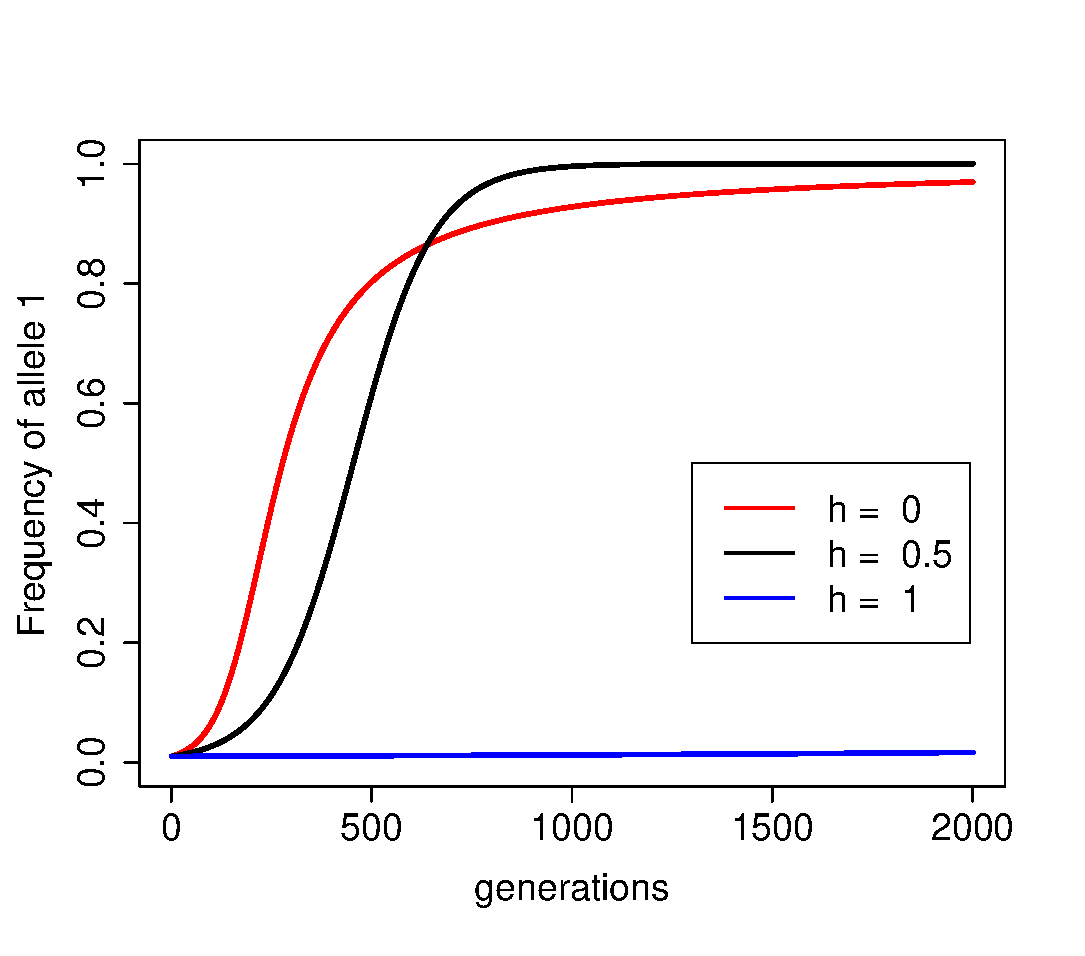
\includegraphics[width=0.5\textwidth]{Figs/simple_diploid_trajs.eps}
\end{center}
\caption{The trajectory of the frequency of allele $A_1$, starting
  from $p_{0}=0.01$, for a selection coefficient $s=0.01$ and three
  different dominance coefficients.}
  \label{fig:diploid_traj}
\end{figure}

\sa{{\bf Question} Comparing the red ($h=0$) and black ($h=0.5$) trajectories in Figure \ref{fig:diploid_traj}, provide an explanation for why $A_1$ increases faster initially if $h=0$, but then approaches fixation more slowly compared to the case of $h=0.5$.}\\

\subsubsection{Heterozygote advantage}
What if the heterozygotes are fitter than either
of the homozygotes? In this case, it is useful to parameterize the relative fitnesses as follows:\\
\begin{center}
\begin{tabular}{lccc}
	genotype & $A_1A_1$ & $A_1A_2$ & $A_2A_2$ \\
	absolute fitness & $w_{11}$ & $<w_{12}>$ & $w_{22}$ \\
	relative fitness (generic) & $w_{11}=W_{11}/W_{12}$ & $w_{12} = W_{12}/W_{12}$ & $w_{22} = W_{22}/W_{12}$ \\
	relative fitness (specific)  & $1-s_1$ & $1$ & $1-s_2$ \\
\end{tabular}\\
\end{center}

Here, $s_1$ and $s_2$ are the differences between the relative fitnesses
of the two homozygotes and the heterozygote. Note that to obtain
relative fitnesses we have divided
absolute fitness by the heterozygote fitness. We could use the
same parameterization as in the model of directional selection, but the reparameterization we have choisen here makes the math prettier.\\

In this case, when allele $A_1$ is rare, it is often found in a
heterozygous state and so it increases in frequency. However, when
allele $A_1$ is common, it is often found in the homozygote state, while
the allele $A_2$ is often found in the heterozygote state; it is
now $A_2$ that increases in frequency at the expense of allele
$1$. Thus, at least in the deterministic model, neither allele can
reach fixation and both alleles will be maintained as a balanced
polymorphism in the population at an equilibrium frequency.\\

We can solve for this equilibrium frequency by setting $\Delta p_t = 0$ in  eqn.\ \eqref{deltap_dip2}, 
i.e.\ $p_tq_t (\wbar_1-\wbar_2)=0$. Doing so, we find that there are three equilibria, all of which are stable. Two of them are not very interesting ($p=0$ or $q=0$), but the third one is the polymorphic equilibrium,  where
$\wbar_1-\wbar_2$ holds.
Using the parametrization above, we see that the marginal fitnesses of the two alleles are formally equivalent. Insertion of the selection coefficients $s_1$ and $s_2$ yields
\begin{equation}
	p_e = \frac{s_2}{s_1+s_2}
\end{equation}
for the equilibrium frequency of interest. This is also the frequency of $A_1$ at which the mean fitness of the population is maximised.\\

\paragraph{Underdominance.} Another case that is of potential interest is the case of fitness
underdominance, where the heterozygote is less fit than either of the
homozygotes. This can be parametrized as follows: \\
\begin{center}
\begin{tabular}{lccc}
	genotype & $A_1A_1$ & $A_1A_2$ & $A_2A_2$ \\
	absolute fitness & $w_{11}$ & $<w_{12}>$ & $w_{22}$ \\
	relative fitness (generic) & $w_{11}=W_{11}/W_{12}$ & $w_{12} = W_{12}/W_{12}$ & $w_{22} = W_{22}/W_{12}$ \\
	relative fitness (specific)  & $1+s_1$ & $1$ & $1+s_2$ \\
\end{tabular}\\
\end{center}

This case also permits three equilibria, $p=0$, $p=1$, and a
polymorphic equilibrium $p=p_U$. However,
now only the first two equilibria are stable, while the polymorphic
equilibrium is unstable. If $p<p_U$ then $\Delta p_t $ is negative
and allele $A_1$ will be lost, while if $p>p_U$, allele
$A_1$ will become fixed.\\

While such alleles might not spread within populations (if $p_U \gg
0$ and selection is reasonably strong), they are of interest in the study of speciation and hybrid
zones. That is because alleles $A_1$ and $A_2$ may have arisen in a
stepwise fashion, i.e.\ not by a single mutation, in separate
subpopulations. Now, heterozygote disadvantage will play a
potential role in species maintenance, \sa{if isolation of the subpopulations is not complete}.\\

\paragraph{Diploid fluctuating fitness}
We would like to think about the case where the diploid absolute fitnesses
are time-dependent. The three genotypes then have fitnesses
$w_{11,t}$, $w_{12,t}$, and $w_{22,t}$ in generation $t$. However,
this case is much less tractable than the haploid case, as segregation
makes it tricky to keep track of the genotype frequencies.  
We can make some progress and gain some intuition by thinking about
how the frequency of allele $A_1$ changes when it is rare.\\
% (This argument is originally due to Haldane and J. )\\

When $A_1$ is rare, i.e.\ $p_t \ll 1$, its frequency in the next
generation \eqref{pgen_dip} can be approximated as
\begin{equation}
p_{t+1} \approx \frac{w_{12}}{\wbar} p_t.
\end{equation}
To obtain this, we have ignored the $p_{t}^2$ term and assumed that $q_t \approx 1$ in the numerator.
Following a similar argument to approximate $q_{t+1}$, we can write
\begin{equation}
	\frac{p_{t+1}}{q_{t+1}} = \frac{w_{12,t}}{w_{22,t}}  \frac{p_{t}}{q_{t}}.
\end{equation}
Then, starting from out from $p_0$ and $q_0$ in generation $0$, $t+1$
generations later, we have
\begin{equation}
	\frac{p_{t+1}}{q_{t+1}} = \left( \prod_{i=0}^{t-1} \frac{w_{12,i}}{w_{22,i}}  \right) \frac{p_{0}}{q_{0}}.
\end{equation}
From this, we can see, following our haploid argument from above, that
the frequency of allele $A_1$ will increase when rare only if
\begin{equation}
	\frac{\sqrt[t]{\prod_{i=0}^{t-1}w_{12,i}}}{\sqrt[t]{\prod_{i=0}^{t-1}w_{22,i}}}>1 \label{geometric_1wins},
\end{equation}
i.e. if the heterozygote has higher geometric mean fitness than the $A_2A_2$ homozygote.\\

The question now is, whether allele $A_1$ will approach fixation in the population,
or whether there are cases in which we can obtain a balanced polymorphism. To investigate that, we can simply repeat our analysis for $q \ll 1$, and see that in that case
\begin{equation}
	\frac{p_{t+1}}{q_{t+1}} = \left( \prod_{i=0}^{t-1} \frac{w_{11,i}}{w_{12,i}}  \right) \frac{p_{0}}{q_{0}}.
\end{equation}
Now, for allele $A_1$ to carry on increasing in frequency and to
approach fixation, the $A_1A_1$ genotype has to be
out-compeeting the heterozygotes. For allele $A_1$ to approach
fixation, we need the geometric mean of $w_{11,i}$ to be greater than the
geometric mean fitness of heterozygotes ($w_{12,i}$).
At the same time, if heterozygotes have higher geometric mean fitness than
the $A_1A_1$ homozygotes, then the $A_2$ allele will increase in frequency when it is rare.
Therefore, a balanced polymorphism can result when the heterozygote
has higher geometric fitness than either of the homozygotes.\\

%\begin{equation}
%\frac{\sqrt[t]{\prod_{i=0}^{t}w_{11,i}}}{\sqrt[t]{\prod_{i=0}^{t}w_{22,i}}}>1
%\end{equation}
%implying that our $11$ homozygotes have to have higher geometric mean
%fitness than our heterozygotes.
%\begin{equation}
%\frac{\sqrt[t]{\prod_{i=0}^{t}w_{11,i}}}{\sqrt[t]{\prod_{i=0}^{t}w_{22,i}}}<1  \label{geometric_2wins}
%\end{equation}
%(satisfying both \eqref{geometric_1wins} and
%\eqref{geometric_2wins}).

Intriguingly, we can have a balanced polymorphism even if the
heterozygote is never the fittest genotype in any generation. To see
this, consider the simple example, where there are two environments
alternate from generation to generation:\\
\begin{tabular}{lccc}
genotype & $A_1A_1$ & $A_1A_2$ & $A_2A_2$ \\
relative fitness in environment A & $w_{11,A}$ & $>w_{12,A}>$ & $w_{22,A}$ \\
relative fitness in environment B  & $w_{11,B}$ & $<w_{12,B}<$ & $w_{22,B}$ \\
Geometric mean fitness & $w_{11,B}$ & $<w_{12,B}>$ & $w_{22}$ \\
\end{tabular}\\

In this case, the polymorphism will remain balanced in the population,
despite the fact that the heterozygote is never the fitest genotype.


\subsection{Mutation--selection balance}
%</source-file>
Mutation is constantly introducing new alleles into the
population. Therefore, variation can be maintained within a
population \sa{not only if selection is balancing (e.g.\ through heterozygote advantage or fluctuating selection over time, as we have seen in the previous section), but also due to} a balance between
mutation \sa{and selection. A case of particular interest is when mutation introduces deleterious} alleles and selection acts against these alleles. To study this balance, we return to the model of directional selection, where allele $A_1$ is advantageous, i.e.
\begin{center}
\begin{tabular}{lccc}
genotype & $A_1A_1$ & $A_1A_2$ & $A_2A_2$ \\
absolute fitness & $W_{11}$ & $ \geq W_{12} \geq$ & $W_{22}$ \\
relative fitness & $w_{11}=1$ & $w_{12}=1-sh$ & $w_{22}=1-s$. \\
\end{tabular}\\
\end{center}

\sa{For a start, we consider the case where allele $A_2$ is not
completely recessive ($h>0$), so that the heterozygotes suffer at least some disadvantage. We denote by $\mu = \mu_{1\rightarrow2}$ the  mutation rate per generation from $A_1$ to the deleterious allele $A_2$, and assume that there is no reverse mutation ($\mu_{2\rightarrow1} = 0$).  Let us assume that selection against $A_2$ is relatively strong compared to the mutation rate, so that it is justified to assume that $A_2$ is always rare, i.e.\ $q_t = 1-q_t \ll 1$. Compared to previous sections, for mathematical clarity, we also switch from following the frequency $p_t$ of $A_1$ to following the frequency $q_t$ of $A_2$. Of course, this is without loss of generality. The change in frequency of $A_2$ due to selection can be written as}
\begin{equation}
	\Delta_S q_t = \frac{\wbar_2 - \wbar_1}{\wbar} p_t q_t  \approx  -hs q_t.
	\label{eq:dirSelApprox}
\end{equation}
This approximation can be found by assuming that $q^2 \approx 0$, $p \approx 1$,
and that $\wbar \approx w_1$. \sa{All of these assumptions make sense if $q \ll 1$. From eqn.\ \eqref{eq:dirSelApprox} we see that selection acts to reduce the frequency of $A_2$ (as both $h$ and $s$ are positive), and it does so geometrically across the
generations. That is, if the initial frequency of $A_2$ is $q_0$, then its frequency at time $t$ is approximately 
\begin{equation}
	q_t = q_0 (1 - hs)^t.
	\label{eq:dirSelExplApprox}
\end{equation}

We will now consider the change in frequency induced by mutation. Recalling that $\mu$ is
the mutation rate from $A_1$ to $A_2$ per generation, the frequency of $A_2$ after mutation
\begin{equation}
	q^{\prime} =  \mu p_t = \mu(1 - q_t).
\end{equation}
Assuming that $\mu \ll 1$ and that $q \ll 1$, the change in the
frequency of allele $A_2$ due to mutation ($\Delta_M q_t$) can be approximated by
\begin{equation}
	\Delta_M q_t = q^{\prime} - q_t =  \mu.
	\label{eq:mutApprox}
\end{equation}
Hence, when $A_2$ is rare and the mutation rate is low, mutation acts to linearly increase the frequency of the deleterious allele $A_2$.\\

If selection is to balance deleterious mutation, there combined effect over one generation has to be zero. Therefore, to find the mutation--selection equilibrium, we set
\begin{equation}
	\Delta_M q_t + \Delta_S q_t = 0,
\end{equation}
insert eqns. \eqref{eq:dirSelApprox} and \eqref{eq:mutApprox}, and solve for $q$ to obtain
\begin{equation}
	q_e = q_t = \frac{\mu}{hs}.
	\label{eqn:mut_sel_bal}
\end{equation}
We see that the frequency of the deleterious allele $A_2$ is balanced at the mutation rate ($\mu$) divided by
the reduction in relative fitness in the heterozygote ($hs$).}\\

\sa{It is worth pointing out that the fitness of the $A_2A_2$ homozygote
has not entered this calculation, as $A_2$ is so rare that it is hardly ever found in the 
homozygous state. Therefore, if $A_2$ has any deleterious effect
in a heterozygous state (i.e.\ if $h>0$) it is this effect that determines the
frequency at which $A_2$ is maintained in the population. Also, note that by
writing the total change in allele frequency as $\Delta_M q_t + \Delta_S q_t
$ we have implicitly assumed that we can ignore terms of order $\mu
\times s$. That is, we have assumed that there is no interaction between mutation and selection. We can do so as we assumed that both $\mu$ and $s$ are small.\\


What effect do such deleterious mutations at mutation--selection balance have on the population? It is common to express this effect in terms of a reduction of the mean relative fitness of the population. For a single site at which a deleterious mutation is segregating at $q_e = \mu/(hs)$, the mean relative fitness is reduced to
\begin{equation}
	\wbar = 1- 2p_e q_e hs - q_e^2s \approx 1-2\mu.
\end{equation}
Somewhat remarkably, the drop in mean fitness due to a site segregating
at mutation--selection balance is independent of the selection coefficient against the
heterozygote; it depends only the mutation rate. Note that this applies only if the mutation is not totally recessive, i.e.\ if $h > 0$.

A reduction of $1 - 2\mu$ is very small, given that the
mutation rate of a gene is likely $<10^{-5}$. However, if there are many loci
segregating at mutation--selection balance, this can accumulate to a substantial so-called
genetic load, and a major cause of variation in fitness-related traits among individuals.

As an aside, if an allele was truly recessive (although few likely are), we have $h=0$, and
so eqn.\ \eqref{eqn:mut_sel_bal} is not valid. However, we can make an argument similar to the one above to show
that, for truly recessive alleles,
\begin{equation}
	q_e = \sqrt{\frac{\mu}{s}}.
\end{equation}
}


\subsubsection{Inbreeding depression}
All else being equal, eqn.\ \eqref{eqn:mut_sel_bal} suggests that mutations that have a smaller effect in the
heterozygote can segregate at higher frequency under mutation--selection balance. As a consequence, alleles that have
strongly deleterious effects in the homozygous state can segregate at
low frequencies in the population, as long as they do not have a
strong effect in heterozygotes. Thus, outbred populations may have many
alleles with recessive deleterious effects segregating within them.

On consequence of this is that inbred individuals from usually outbred
populations may have dramatically lower fitnesses than outbred
individuals. This is a consequence of being homozygous at many loci for
alleles with recessive deleterious effects. Indeed, this seems to be a common observation, dating back to systematic surveys by
Darwin. In typically outbred populations, the mean fitness of individuals
decreases with the inbreeding coefficient, i.e.\ this so-called inbreeding depression
is a common observation.

\paragraph{Purging the inbreeding load.}
That said, populations that regularly inbreed over sustained periods of time
are expected to partially purge this load of deleterious
alleles. This is because such populations have exposed many of these alleles
in a homozygous state, and so selection can more readily remove these alleles
from the population.

\newpage
\subsection{Migration--selection balance}
Another reason for the persistence of deleterious alleles in a
population is that there is a constant influx of maladaptive alleles
from other populations where these alleles are locally adapted.
This seems unlikely to be as broad an explanation for the
persistence of deleterious alleles genome-wide as mutation-selection
balance. However, a brief discussion of such alleles is worthwhile as
it helps to inform our ideas about local adaptation.\\

As a first pass at this lets consider a haploid two allele model with
two different populations, where the relative fitnesses of our alleles
are as follows
\begin{center}
\begin{tabular}{c|cc}
allele & $1$ & $2$ \\
\hline
population 1 & 1 & 1-s \\
population 2 & 1-s & 1 \\
\end{tabular}
\end{center}
As a simple model of migration lets suppose within a population a
fraction of $m$ individuals are migrants from the other population,
and $1-m$ individuals are from the same deme.\\

To quickly sketch a solution to this well set up a situation analogous
to our mutation-selection balance model. to do this lets assume that selection is strong compared to migration ($s \gg m$) then allele
$1$ will be almost fixed in population $1$ and allele $2$ will be
almost fixed in population $2$. If that is the case,
migration changes the frequency of allele $2$ in population $1$ ($q_1$) by
\begin{equation}
\Delta_{Mig.} q_1 \approx m
\end{equation}
while as noted above $\Delta_{S} q_1= -sq_1$, so that migration and
selection are at an equilibrium when $\Delta_{S} q_1+
\Delta_{Mig.}q_1$, i.e. an equilibrium frequency of allele $2$ in
population $1$ of
\begin{equation}
q_{e,1} = \frac{m}{s}
\end{equation}
so that migration is playing to role of mutation and so
migration-selection balance (at least under strong selection) is
analogous to mutation selection balance.\\

\subsubsection{Some theory of the spatial distribution of allele
frequencies under deterministic models of selection}
Imagine a continuous haploid population spread out along a line. 
individual dispersals a random distance $\Delta x$ from its birthplace to the
location where it reproduces, where $\Delta x$ is drawn from the probability
density $g(~)$. To make life simple we will assume that $g(\Delta x)$
is normally distributed with mean zero and standard deviation
$\sigma$, i.e. migration is unbiased an individuals migrate an average
distance of $\sigma$. \\

Our frequency of allele $2$ at time $t$ in the population at spatial
location $x$ is $q(x,t)$. Assuming that only dispersal occurs, how
does our allele frequency change in the next generation. Our allele
frequency in the next generation at location $x$ reflects
the migration from different locations in the proceeding
generation. Our population at location $x$ receives a contribution
$g(\Delta x)q(x+\Delta x,t)$ of allele $2$ from the population at location $x+\Delta x$,
such that the frequency of our allele at $x$ in the next generation is
\begin{equation}
q(x,t+1) = \int_{-\infty}^{\infty} g(\Delta x)q(x+\Delta x,t) d \Delta x.
\end{equation}
To obtain
$q(x+\Delta x,t)$ lets take a taylor series expansion of $q(x,t)$
\begin{equation}
q(x+\Delta x,t) = q(x,t) + \Delta x \frac{dq(x,t)}{dx}+ \tfrac{1}{2}(\Delta x)^2 \frac{d^2q(x,t)}{dx^2}+\cdots
\end{equation}
then
\begin{equation}
q(x,t+1) = q(x,t) +\left( \int_{-\infty}^{\infty} \Delta x g(\Delta x) 
  d \Delta x \right) \frac{dq(x,t)}{dx} + \tfrac{1}{2}\left( \int_{-\infty}^{\infty}(\Delta x)^2 g(\Delta x) 
  d \Delta x \right)  \frac{d^2q(x,t)}{dx^2}+\cdots
\end{equation} 
$g(~)$ has a mean of zero so $ \int_{-\infty}^{\infty} \Delta x g(\Delta x) 
  d \Delta x =0$ and has variance $\sigma^2$ so $\int_{-\infty}^{\infty}(\Delta x)^2 g(\Delta x) 
  d \Delta x = \sigma^2$ and all higher terms are zero (as all high
  moments of the normal are zero). Looking at the change in frequency $\Delta
  q(x,t) = q(x,t+1)-q(x,t+1)$ then 
\begin{equation}
\Delta q(x,t) = \frac{\sigma^2}{2} \frac{d^2q(x,t)}{dx^2}
\end{equation} 
this is a diffusion equation, so that migration is acting to smooth
out allele frequency differences with a diffusion constant
of $\tfrac{\sigma^2}{2}$. This is exactly analogous to the equation
describing how a gas diffuses out to equal density, as both particles
in a gas and our individuals of type $2$ are performing brownian
motion (blurring our eyes and seeing time as continuous). \\


We will now introduce fitness differences into our model and set the
relative fitnesses of allele $1$ and $2$ at location $x $ to be $1$ and
$1+s\gamma(x)$. To make progress in this model we'll have to assume that selection
isn't too strong i.e. $s \gamma(x) \ll 1$ for all $x$. The the change in
frequency of allele $2$ obtained within a generation due to selection is
\begin{equation}
q^{\prime}(x,t) - q(x,t) \approx s\gamma(x) q(x,t) \big( 1 - q(x,t) \big)
\end{equation}
i.e. logistic growth of our favoured allele at location $x$. 
Putting our selection and migration terms together we find 
\begin{equation}
q(x,t+1) - q(x,t) = s\gamma(x) q(x,t) \big( 1 - q(x,t)
\big)+\frac{\sigma^2}{2} \frac{d^2q(x,t)}{dx^2} \label{eqn:fisherKPP}
\end{equation}
in derving this we have essentially assumed that migration acted upon our original
frequencies before selection and in doing so have ignored terms of the
order of $\sigma s$. 


\begin{figure}
\begin{center}
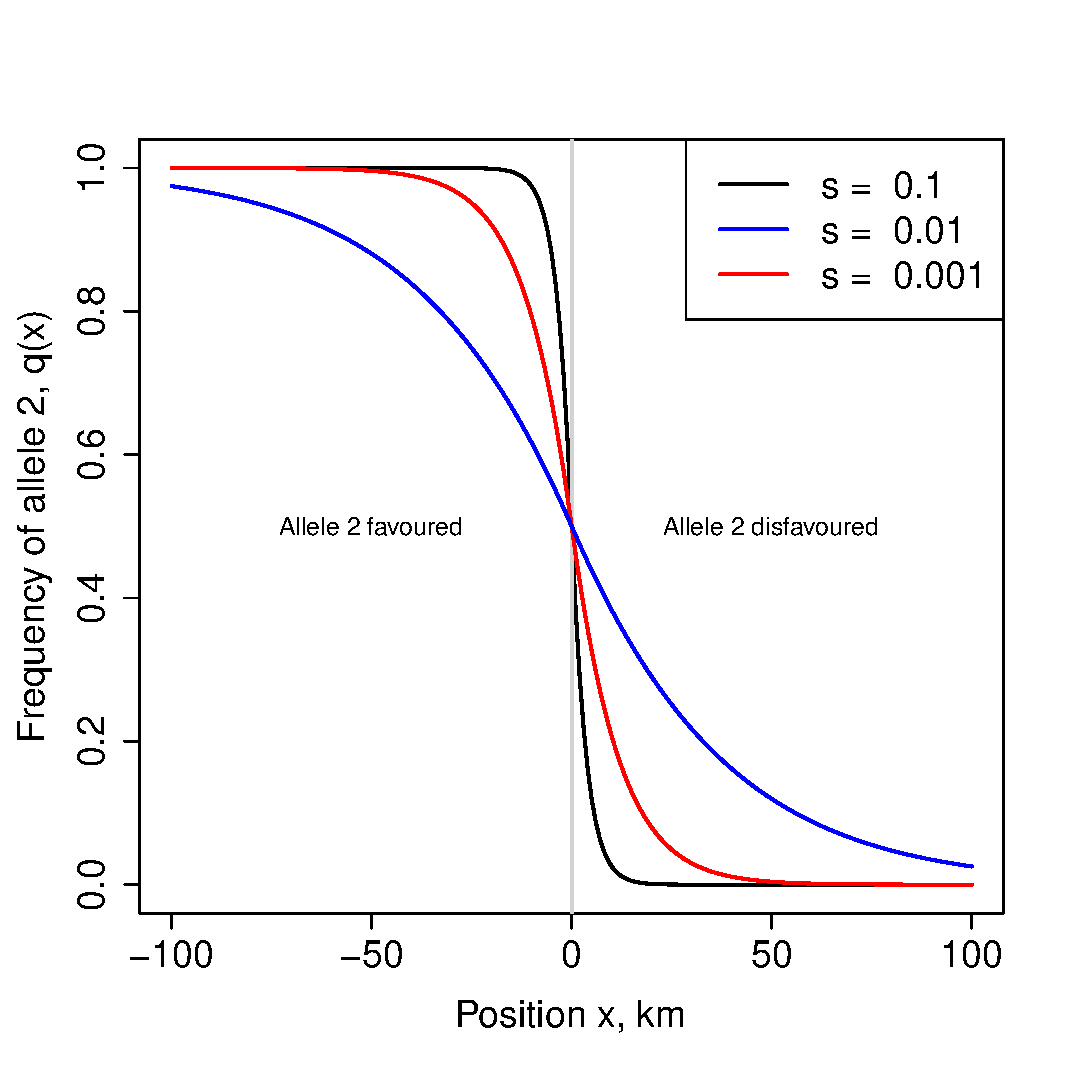
\includegraphics[width=0.5\textwidth]{Figs/equilib_cline.eps}
\end{center}
\caption{An equilibrium cline in allele frequency. Our individuals
  dispersal an average distance of $\sigma=1$km per generation, and our
allele $2$ has a relative fitness of $1+s$ and $1-s$ on either side of
the environmental change at $x=0$.} \label{fig:cline}
\end{figure}


To make progress lets consider a simple model of location adaptation
where the environment abruptly changes. Specifically we assume that
$\gamma(x)= -1$
for $x<0$ and $\gamma(x)= 1$ for $x \geq 0$, i.e. our allele $2$ has a
selective advantage at locations to the left of zero, while this
allele is at a disadvantage to the right of zero. In this case we can
get an equilibrium distribution of our two alleles were to the left
of $zero$ our allele $2$ is at higher frequency, while to the right of
zero allele $1$ predominates. As we cross from the left to the right
side of our range the frequency of our allele $2$ decreases in a
smooth cline.\\



%Under such a model the change in frequency of allele $2$ at location $x$ at time $t$,
%$q(x,t)$, over time follows the differential equation
%\begin{equation}
%\frac{dq(x,t)}{dt} = s\gamma(x) q(x,t) \left( 1 - q(x,t) \right) + \frac{\sigma^2}{2} \frac{d^2q(x,t)}{dx^2}
%\end{equation}
%the first term on the right-hand side is the logistic growth of our
%favoured allele at location $x$, while the second term on the
%right-hand side is the diffusion of allele frequencies due to
%dispersal (i.e. dispersal is acting to spread out the effect of
%allele frequency change across populations). See below for how we
%derive this \gc{to be added}.\\

Our equilibrium spatial distribution of allele frequencies can be found by
setting the LHS of eqn. \eqref{eqn:fisherKPP} to zero to arrive at
\begin{equation}
s\gamma(x) q(x) \left( 1 - q(x) \right) = \frac{\sigma^2}{2} \frac{d^2q(x)}{dx^2}
\end{equation}
We then could solve this differential equation with appropriate boundary
conditions ($q(-\infty)=1$ and $q(\infty) = 0$) to arrive at the
appropriate functional form to our cline. While we won't go into the
solution of this equation here, we can note that by dividing our
distance $x$ by $\ell=\sigma/\sqrt{s}$ we can remove the effect of our
parameters from the above equation. This compound parameter $\ell$ is the characteristic
length of our cline, and it is this parameter which determines over
what geographic scale we change from allele $2$ predominating to
allele $1$ predominating as we move across our environmental shift. \\

The width of our cline, i.e. over what distance do we make this shift
from allele $2$ predominating to allele $1$,
can be defined in a number of different ways. One simple way to define
the cline width, which is easy to define but perhaps hard to measure accurately, is the slope (i.e. the
tangent) of $q(x)$ at $x=0$. Under this definition the cline width is approximately $0.6
\sigma/\sqrt{s}$.\\

\newpage
\section{Stochasticity and Genetic Drift in allele frequencies}
\subsection{Stochastic loss of strongly selected alleles}
% Fisher (1922, 1930) and Haldane (1927)
Even strongly selected alleles can be lost from the population when
they are sufficiently rare. This is because the number of offspring
left by individuals to the next generation is fundamentally
stochastic. A selection coefficient of s=$1\%$ is a strong
selection coefficient, which can drive an allele through the
population in a few hundred generations once the allele is
established. However, if individuals have on average a small number of
offspring per generation the first individual to carry our allele who
has on average $1\%$ more children could easily have zero offspring, leading to the loss
of our allele before it ever get a chance to spread.\\

To take a first stab at this problem lets think of a very large
haploid population, and in order for this population to stay constant in size
we'll assume that individuals without the selected mutation have on average one
offspring per generation. While individuals with our selected allele
have on average $1+s$ offspring per generation. We'll assume that the
distribution of offspring number of an individual is Poisson
distributed with this mean, i.e. the probability that an individual
with the selected allele has $i$ children is
\begin{equation}
P_i= \frac{(1+s)^i e^{-(1+s)}}{i!}
\end{equation}

Consider starting from a single individual with the selected allele, and ask
about the probability of eventual loss of our selected allele starting
from this single copy ($p_L$). To derive this we'll make use of a
simple argument (derived from branching processes). Our selected
allele will be eventually lost from the population if every individual
with the allele fails to leave descendents.
\begin{enumerate}
\item In our first generation
with probability $P_0$ our individual leaves no copies of itself to
the next generation, in which case our allele is lost.
\item Alternatively
it could leave one copy of itself to the next generation (with
probability $P_1$), in which
case with probability $p_L$ this copy eventually goes extinct.
\item It could leave two copies of itself to the next generation (with
probability $P_2$), in which
case with probability $p_L^2$ both of these copies eventually goes extinct.
\item More generally it could leave could leave $k$ copies ($k>0$) of itself to the next generation (with
probability $P_k$), in which case with probability $p_L^k$  all of these copies eventually go extinct.
\end{enumerate}
summing over this probabilities we see that
\begin{eqnarray}
p_L &= \sum_{k=0}^{\infty} P_k p_L^{k}  \nonumber \\
&=  \sum_{k=0}^{\infty} \frac{(1+s)^ke^{-(1+s)}}{k!} p_L^{k} \nonumber
\\
&= e^{-(1+s)} \left( \sum_{k=0}^{\infty} \frac{\left(p_L(1+s) \right)^k}{k!}  \right)
\end{eqnarray}
well the term in the brackets is itself an exponential expansion, so
we can rewrite this as
\begin{equation}
p_L = e^{(1+s)(p_L-1)} \label{prob_loss}
\end{equation}
solving this would give us our probability of loss for any selection
coefficient. Lets
rewrite this in terms of the the probability of escaping loss $p_F = 1-p_L$.  We can
rewrite eqn \eqref{prob_loss} as
\begin{equation}
1-p_F = e^{-p_F(1+s)}
\end{equation}
to gain an approximation to this lets consider a small selection
coefficient $s \ll 1$ such that $p_F \ll 1$ and then expanded out the
exponential on the right hand side (ignoring terms of higher
order than $s^2$ and $p_F^2$) then
\begin{equation}
1-p_F \approx 1-p_F(1+s)+p_F^2(1+s)^2/2
\end{equation}
solving this we find that
\begin{equation}
p_F = 2s.
\end{equation}
Thus even an allele with a $1\%$ selection coefficient has a $98\%$
probability of being lost when it is first introduced into the
population by mutation. \\

%%consider reparameterizing 1+(1-hs)s
We can also adapt this result to a diploid setting.
Assuming that heterozygotes for the $1$ allele have $1+(1-h)s$ children, the
probability of allele $1$ is not lost, starting from a single copy in
the population, is
\begin{equation}
p_F = 2 (1-h)s \label{eqn:diploid_escape}
\end{equation}
for $h>0$.\\


\subsection{The interaction between genetic drift and weak selection.}
For strongly selected alleles, once the allele has escaped initial
loss at low frequencies, their path will be determined deterministically by their
selection coefficients. However, if selection is weak the
stochasticity of reproduction can play a role in the trajectory an
allele takes even when it is common in the population.\\

To see this lets think of our simple Wright-Fisher model (see R
exercise). Each generation we allow a deterministic change in our
allele frequency, and then binomially sample two alleles for each of
our offspring to construct our next generation.\\


%%%%%Include this discussion of sampling back in our HWE section??
%%%%%Next time

So the expected change in our allele frequency within a generation is given just by our
deterministic formula. To make things easy on our self lets assume an
additive model, i.e. $h=1/2$, and that $s \ll 1$ so that $\wbar
\approx 1$. This gives us
\begin{equation}
\E(\Delta p ) = \frac{s}{2} p(1-p) \label{eqn:WF_mean}
\end{equation}
our variance in our allele frequency change is given by
\begin{equation}
Var(p^{\prime} - p) = Var(p^{\prime}) = \frac{p^{\prime}(1-p^{\prime})}{2N}
\end{equation}
this variance in our allele frequency follows from the fact that we
are binomially sampling $2N$ new alleles in the next
generation from a frequency $p^{\prime}$. Denoting our count of allele $1$ by $i$ our
\begin{equation}
Var(p^{\prime} - p) = Var(\frac{i}{2N} - p) =  Var(\frac{i}{2N} ) =\frac{Var(i)}{(2N)^2}
\end{equation}
and from binomial sampling $Var(i) = 2N p^{\prime}(1-p^{\prime})$ and
so we arrive at our answer. Assuming that $s \ll 1$, $p^{\prime}
\approx p$, then in practice we can use
\begin{equation}
Var(\Delta p)  =Var(p^{\prime} - p) \approx \frac{p(1-p)}{2N}. \label{eqn:WF_var}
\end{equation}
To get our first look at the relative effects of selection vs drift we
can simply look at when our change in allele frequency caused
selection within a generate is reasonably faithfully passed across
the generations. In particular if our expected change in frequency is much
great than the variance around this change, genetic drift will play
little role in the fate of our selected allele (once the allele is not
too rare within the population). When does selected
dominant genetic drift? This will happen if $\E(\Delta p) \gg Var(\Delta p)$ when $Ns \gg 1$. Conversely any
hope of our selected allele following its deterministic path will be quickly undone if our change in allele frequencies due to selection is
much less than the variance induced by drift. So if $Ns \ll 1$ then
drift will dominate the fate of our allele. \\


To make further progress on understanding the fate of alleles with
selection coefficients of the order $1/N$ requires more careful
modeling. However, we can obtain the probability that under our diploid model, with an additive selection coefficient $s$, the
probability of allele $1$ fixing within the population starting
from a frequency $p$ is given by
\begin{equation}
\pi(p) = \frac{1-e^{-2Ns p }}{1-e^{-2Ns}} \label{eqn:prob_fixed}
\end{equation}
the proof of this is sketched out below (see Section \ref{Section:fixation_weakly_sel}). A new allele will arrive in the population at frequency $p=1/(2N)$,
then its probability of reaching fixation is
\begin{equation}
\pi \left(\frac{1}{2N} \right) = \frac{1-e^{-s }}{1-e^{-2Ns}}
\end{equation}
if $s \ll1$ but $Ns \gg 1$ then $\pi(\frac{1}{2N}) \approx s$, which
nicely gives
us back our result that we obtained above
(eqn. \eqref{eqn:diploid_escape}).\\

In the case where $Ns$ close to $1$ then
\begin{equation}
\pi(\frac{1}{2N}) \approx \frac{s}{1-e^{-2Ns}} \label{eqn:escape_from_intro}
\end{equation}
this is greater than $s$, increasingly so for smaller $N$.
Why is this? Well in small populations selected alleles spend a
somewhat shorter time segregating (especially at low frequencies), and so are
slightly less susceptible to genetic drift. \\

\subsubsection{The fixation of slightly deleterious alleles.}
We can also use eqn. \eqref{eqn:escape_from_intro} to understand how
likely it is that deleterious alleles accidently reach fixation by
genetic drift, assuming a diploid model with additive selection (with
a selection coefficient of $-s$ against our allele $2$).  
If $N s \gg 1$ then our deleterious allele (allele $2$) can not possibly reach
fixation. However, if $Ns$ is not large then
\begin{equation}
\pi(\frac{1}{2N}) = \frac{s}{e^{2Ns}-1} \label{eqn:fix_deleterious}
\end{equation}
for our deleterious allele. So deleterious alleles can fix within
populations (albeit at a low rate) if $Ns$ is not too large.\\

\subsubsection{A Sketch Proof of the probability of fixation of
weakly selected alleles} \label{Section:fixation_weakly_sel}
%Kolmogorov backward eqn. 1931
%Kimura, M. 1962 On the Probability of Fixation of Mutant Genes in a
%Population. for abitrary dominance in diffusion.

We'll let $P(\Delta p)$ be the probability that our allele frequency
shifts by $\Delta p$ in the next generation. Using this we can write our probability $\pi(p)$ in terms of the probability of
achieving fixation averaged over the frequency in the next generation
\begin{equation}
\pi(p)  = \int \pi(p+\Delta p) P(\Delta p) d(\Delta p) \label{eqn:prob_fix_diff_step1}
\end{equation}
This is very similar to the technique that we used deriving our
probability of escaping loss in a very large population above. \\

So we need an expression for $\pi(p+\Delta p)$. To obtain this we'll
do a Taylor series expansion of $\pi(p)$ assuming that $\Delta p $ is small
\begin{equation}
\pi(p+\Delta p) \approx \pi(p) + \Delta p \frac{d\pi(p)}{dp} + (\Delta p)^2
\frac{d^2\pi(p)}{dp^2} (p)
\end{equation}
ignoring higher order terms.\\

Taking the expectation over $\Delta p $ on both sides, as in
eqn. \ref{eqn:prob_fix_diff_step1}, we obtain
\begin{equation}
\pi(p) = \pi(p) + \E(\Delta p) \frac{d\pi (p)}{dp} + \E((\Delta p)^2)
\frac{d^2\pi(p)}{dp^2}
\end{equation}

Well $\E(\Delta p) = \frac{s}{2}p(1-p)$ and $Var(\Delta p)= \E(\Delta
p)^2)-\E^2(\Delta p)$, so if $s \ll 1$ then $\E^2(\Delta p) \approx
0$, and $\E(\Delta p)^2 = \frac{p(1-p)}{2N}$. This leaves us with
\begin{equation}
0= \frac{s}{2}p(1-p)\frac{d\pi (p) }{dp} + \frac{p(1-p)}{2N}
\frac{d^2\pi (p) }{dp^2}
\end{equation}
and we can specify the boundary conditions to be $\pi(1)=1$ and $\pi(0)=0$. 
Solving this differential equation is somewhat involved process but in
doing so we find that
\begin{equation}
\pi(p) = \frac{1-e^{-2Ns p }}{1-e^{-2Ns}}
\end{equation}


\section{Genetic drift and Neutral alleles}



\subsection{The fixation of neutral alleles}
It is very unlikely that a rare neutral allele accidentally drifts up
to fixation, it is much more likely that such an allele is eventually
is lost from the population. However, there is a large and constant influx of
rare alleles into the population due to mutation, so even if it is very
unlikely that an individual allele fixes within the population, some
neutral alleles will fix.  \\

%We'll first consider the probability that a neutral allele fixes
%within the population, starting from it just enters a diploid
%population as a newly mutated allele at frequency $1/(2N)$.

%so for an allele to be fixed in the population it
%must have been that allele


\paragraph{Probability of the eventual fixation of a neutral allele.} An allele which reaches fixation within a population, is an ancestor to
the entire population. In a particular generation there can be only single
allele that all other alleles at the locus in  later generation can claim as a
ancestor. As at a neutral locus all of our alleles are exchangeable, as
they have no effect on the number of descendents an individual
leaves, so any allele is equally likely to be the ancestor of the
entire population.  In a diploid population size of size $N$, there are $2N$
alleles all of which are equally likely to be the ancestor of the
entire population at some later time point. So if our allele is present in a single copy, the chance that
is the ancestor to the entire population in some future generation is
$1/(2N)$, i.e. the chance our neutral allele is eventually fixed is
$1/(2N)$.\\

More generally if our neutral allele is present in $i$ copies in the
population, of $2N$ alleles, the probability that this allele is fixed
is $i/(2N)$. I.e. the probability that a neutral allele is eventually
fixed is simply given by its frequency ($p$) in the population.
We can also derive this result by letting $Ns \rightarrow
0$ in eqn. \eqref{eqn:prob_fixed}.

\paragraph{Rate of substitution of neutral alleles.}

A substitution between populations that do not exchange gene flow is
simply a fixation event within one population. The rate of
substitution is therefore the rate at which new alleles fix in the
population, so that the long-term substitution rate is the rate at
which mutations arise that will eventually become fixed within our population.\\

Assume that there are two classes of mutational changes that can occur with a
region, highly deleterious mutations and neutral mutations. A fraction
$C$ of all mutational changes are highly deleterious, and can not
possibly contribute to substitution nor polymorphism (i.e. $Ns \gg 1$).
While a fraction $1-C$ are neutral. If our mutation rate is $\mu$ per
transmitted allele per generation, then a total of $2N \mu (1-C)$
neutral mutations enter our population each generation.\\

Each of these neutral mutations has a $1/(2N)$ probability chance of
eventually becoming fixed in the population. Therefore, the rate at
which neutral mutations arise that eventually become fixed within our
population is  
\begin{equation}
2N\mu(1-C)\frac{1}{2N} = \mu(1-C)
\end{equation}
thus the rate of substitution under a model where newly arising alleles are either
highly deleterious or neutral, is simply given by the mutation rate
towards neutral alleles, i.e. $\mu(1-C)$.\\

Consider a pair of species have diverged for $T$ generations, i.e. orthologous sequences shared between the species last shared a common ancestor $T$ generations ago. If they have maintained a constant $\mu$ over that time, will have accumulated an average of
\begin{equation}
2\mu(1-C)T
\end{equation}
neutral substitutions. This assumes that $T$ is a lot longer than the time it
takes to fix a neutral allele, such that the total number of 
alleles introduced into the population that will eventually fix is the
total number of substitutions. We'll see below that a neutral allele
takes on average $4N$ generations to fix from its introduction into
the population.\\

This is a really pretty result as the population size has completely
canceled out of the neutral substitution rate. However, there is
another way to see this in a more straightward way. If I look at a
sequence in me compared to say a particular chimp, I'm looking at the mutations
that have occurred in both of our germlines since they parted ways $T$
generations ago. Since neutral alleles do not alter the probability
of their transmission to the next generation, we are simply looking at
the mutations that have occurred in $2T$ generations worth of
transmissions. Thus the average number of neutral mutational
differences separating our pair of species is simply $2\mu (1-C) T$.\\


\subsection{The Coalescent and patterns of neutral diversity}

\paragraph{Pairwise Coalescent time distribution and the number of
 pairwise differences.}
Thinking back to our calculations we made about the loss of neutral heterozygosity
and equilibrium levels of diversity (in Sections \ref{LossofHet} and \ref{DriftMutationBalance}), you'll note that we could first specify
what generation a pair of sequences coalesce in, and then calculate
some properties of heterozygosity based on that. That's because neutral
mutations do not affect the probability that an individual transmits
that allele, so don't affect the way in which we can trace ancestral lineages
back. \\

As such it will often be helpful to consider the time to the common
ancestor of a pair of sequences, and then think of the impact of that
on patterns of diversity. See Figure \ref{fig:Coalescent_simulation}
for an example of this. The probability that a pair of alleles
have failed to coalesce in $t$ generations and then coalesce in the
$t+1$ generation back is
\begin{equation}
\frac{1}{2N} (1- \frac{1}{2N} )^{t} \approx \frac{1}{2N} e^{-t/(2N)} \label{eqn:coal_time_dist}
\end{equation}
thus the coalescent time of a pair of sequences ($T_2$) is
approximately exponentially distributed with a rate $1/(2N)$. We'll denote that by
saying that $T_2 \sim Exp \left( 1/(2N) \right)$. The mean coalescent
time of a pair of a pair of alleles is $2N$ generations\\


\begin{figure}
\begin{center}
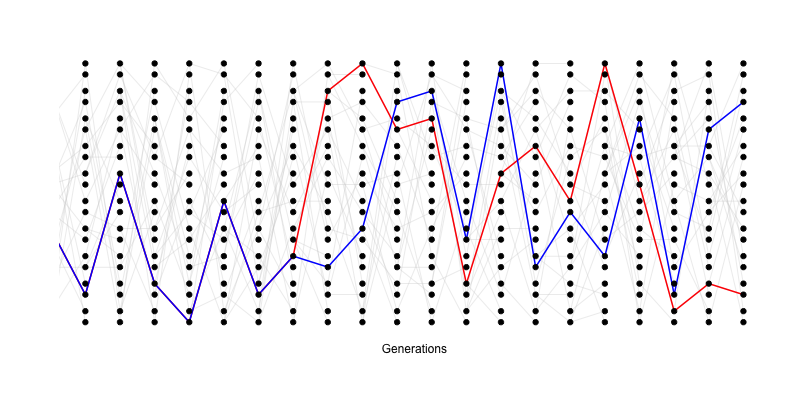
\includegraphics[width=\textwidth]{Figs/Coalescent.png}
\end{center}
\caption{A simple simulation of the coalescent process. The simulation
  consists of a diploid population of 10 individuals (20 alleles). In
  each generation, each individual is equally likely to be the parent
  of an offspring (and the allele transmitted is indicated by a light
  grey line).  We track a
  pair of alleles, chosen in the present day, back 14 generations
  untill they find a common ancestor.} \label{fig:Coalescent_simulation}
\end{figure}



Conditional on a pair of alleles coalescing $t$ generations ago
there are $2t$ generations in which a mutation could occur. Thus the
probability of our pair of alleles are separated by $j$ mutations
since they last shared a common ancestor is
\begin{equation}
P(j | T_2 = t ) = {2t \choose j} \mu^{j} (1-\mu)^{2t-j}
\end{equation}
i.e. mutations happen in $j$ generations, and do not happen in $2t-j$
generations (with ${2t \choose j}$ ways this can possibly
happen). Assuming that $\mu \ll 1$, and that $2t-j \approx 2t$ then we
can approximate the probability that we have $j$ mutations as a
Poisson distribution
\begin{equation}
P(j | T_2 = t ) = \frac{ (2 \mu t )^{j} e^{-2\mu t}}{j!}
\end{equation}
i.e. a Poisson with mean $2\mu t $. \\

As our expected coalescent time is $2N$ generations, the expected
number of mutations separating two alleles drawn at random from the
population is
\begin{equation}
\E(j) = 4N\mu = \theta
\end{equation}
We'll assume that mutations never happen at the same site twice,
i.e. no multiple hits, such that we get to see all of the mutation events that separate our pair
of sequences (we'll call this the infinitely-many-sites assumption,
which should be fine if $N\mu_{BP} \ll 1$). Thus the number of
mutations between a pair of sites is the observed number of
differences between a pair of sequences. \\


We'll denote the observed number of pairwise differences at putatively
neutral sites separating a
pair of sequences as $\pi$ (we usually average this over a number of
pairs of sequences for a region). So we can estimate of
$\theta$ from $\pi$, $\widehat{\theta}_{\pi}$ by setting $\widehat{\theta}_{\pi}=\pi$.
If we have an independent
estimate of $\mu$, then from setting $\pi = \widehat{\theta}_{\pi} = 4N\mu$ we can obtain an
estimate of the population size $N$ that is consistent with our levels
of neutral polymorphism.



\subsection{The coalescent process of a sample of alleles.}

Usually we are not just interested pairs of alleles, or the
average pairwise diversity, we are interested in the properties of
diversity in samples of a number of alleles drawn from the population.  
To allow for this instead of just following a pair of lineages back until they
coalesce, we can follow the history of a sample of alleles back
through the population.

Consider first sampling three alleles at random from the
population. The probability that all three alleles choose exactly the
same ancestral allele one generation back is $1/(2N)^2$. If $N$ is
reasonably large then this is a very small probability. As such it is
very unlikely that our three alleles coalesce at once, a in a moment
we'll see that it is safe to ingnore such unlikely events. \\

The
probability that a specific pair of alleles find a common ancestor in
the preceding generation is still $1/(2N)$. There are three possible
pairs of alleles so the probability that no pair finds a common
ancestor is
\begin{equation}
\left(1-\frac{1}{(2N)} \right)^3 \approx \left( 1- \frac{3}{2N} \right)
\end{equation}
in making this approximation we are multiplying out the right hand-side
and ignoring terms of $1/N^2$ and higher. See
Figure \ref{fig:Coalescent_simulation_3} for a random realization of this process. \\


\begin{figure}
\begin{center}
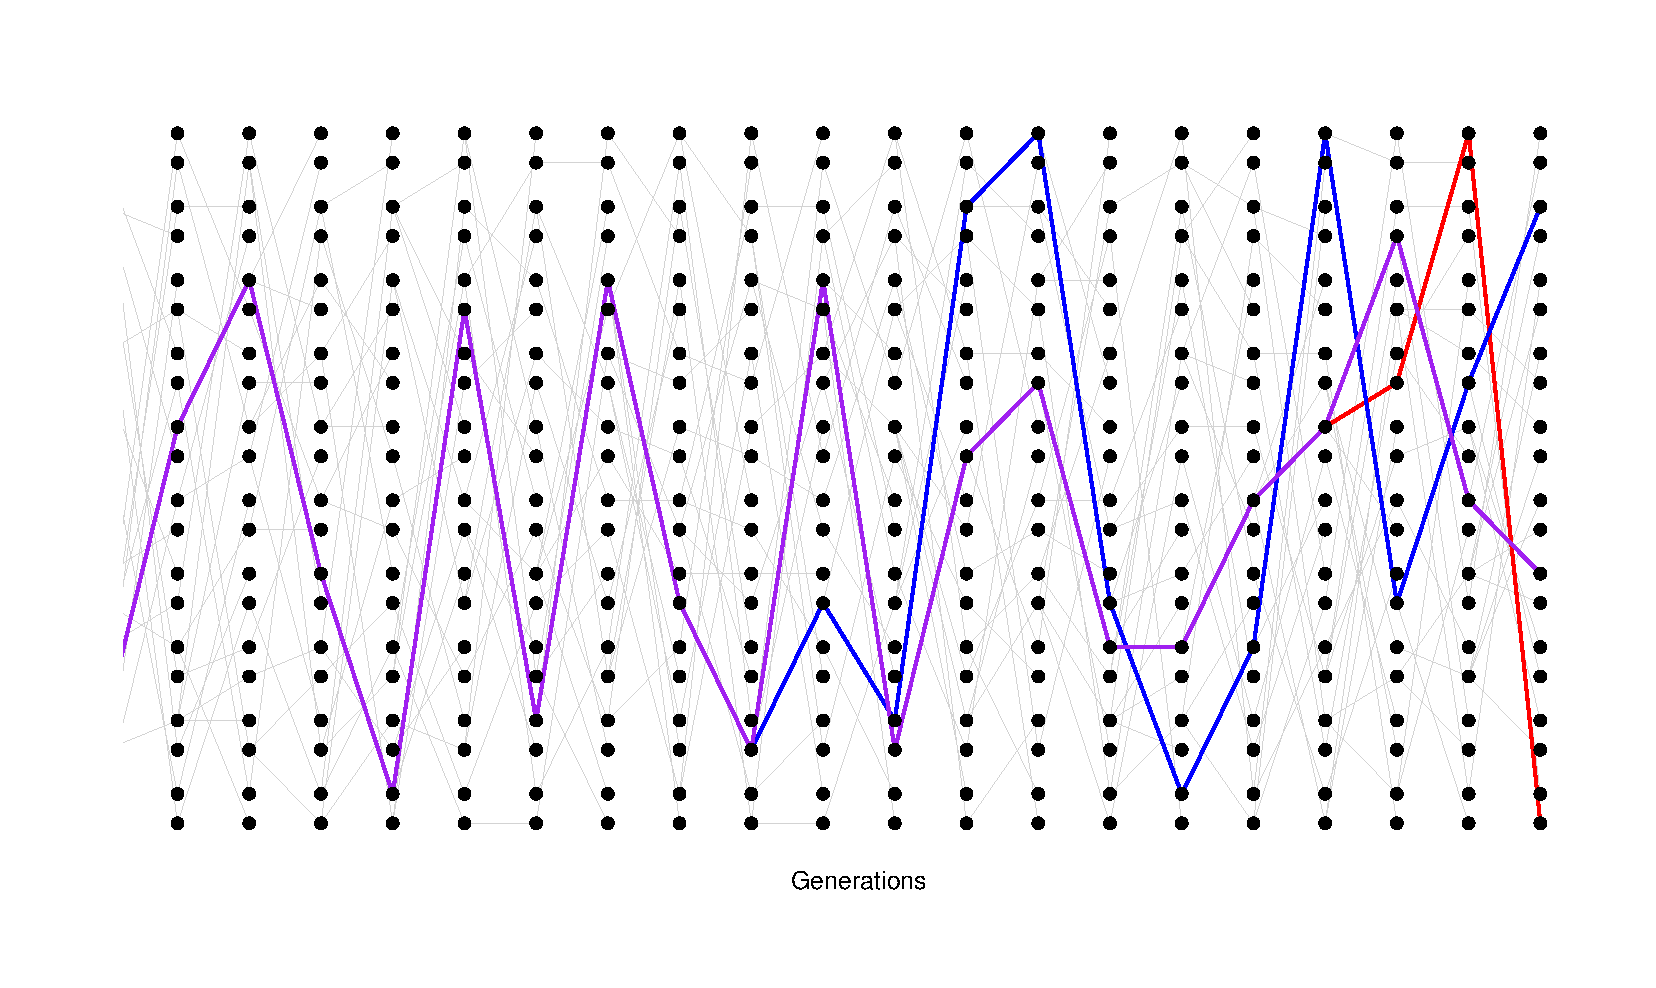
\includegraphics[width = \textwidth]{Figs/Coalescent_3}
\end{center}
\caption{A simple simulation of the coalescent process for three
  lineages. We track the ancestry of 
  three modern-day alleles, the first pair (blue and purple) coalesce four generations back 
  their are then two independent lineages we are tracking, this pair
  then coalesces twelve generations in the past. Note that different
  random realizations of this process will differ from each other a lot.} \label{fig:Coalescent_simulation_3}
\end{figure}


More generally when we sample $i$ alleles there are ${i \choose
 2}$ pairs, i.e. $i(i-1)/2$ pairs, thus the probability that no pair
of alleles coalesces in the preceding generation is
\begin{equation}
\left(1-\frac{1}{(2N)} \right)^{{i \choose
 2}} \approx \left( 1- \frac{{i \choose
 2}}{2N}\right)
\end{equation}
while the probability of any pair coalescing is $\approx \frac{{i \choose
 2}}{2N}$.\\

We can ignore the possibility of more than pairs of alleles (e.g. tripletons) simultaneously
coalescing at once as terms of $1/N^2$ and higher can
be ignored as they are vanishingly rare. Obviously there are in reasonable sample sizes there are
many more triples (${i \choose 3}$), and higher order combinations, than pairs
(${i \choose 2}$) but if $i \ll N$ then we are safe to
ignore these terms.

When there are $i$ alleles the probability that we wait until the
$t+1$ generation before
any pair of alleles coalesce is
\begin{equation}
 \frac{{i \choose
 2}}{2N}\left( 1- \frac{{i \choose
 2}}{2N}\right)^{t-1} \approx  \frac{{i \choose
 2}}{2N} \exp \left( - \frac{{i \choose
 2}}{2N} t \right)
\end{equation}
thus the waiting time $T_i$ to the first coalescent event in a sample
of $i$ alleles is exponentially distributed with rate $\frac{{i \choose
 2}}{2N}$, i.e. $T_i \sim Exp\left(\frac{{i \choose
 2}}{2N} \right)$. The mean waiting time till any of pair within our
sample to coalesce is $2N/{i \choose
 2}$.\\

When a pair of alleles first find a common ancestral allele some
number of generations back further into the past we only have to keep
track of that common ancestral allele for the pair. Thus when a pair
of alleles in our sample of $i$ alleles coalesce, we then switch to
having to follow $i-1$ alleles back. Then when a pair of these $i-1$
alleles coalesce, we then have to follow $i-2$ alleles back. This
process continues until we coalesce back to a sample of two, and from
there to a single most recent common ancestor (MRCA).\\


To simulate a coalescent genealogy at a locus for a sample of $n$ alleles we therefore simply follow this
algorithm
\begin{enumerate}
\item set $i=n$.
\item We simulate a random variable to be the time $t_i$ to the next coalescent event from $t_i \sim
 Exp\left(\frac{{i \choose
 2}}{2N} \right)$
\item choose a pair of alleles to coalesce at random from all possible
 pairs.
\item set $i=i-1$
\item continue looping of steps 1-3 until $i=1$ i.e. the most recent
 common ancestor of the sample is found.
\end{enumerate}
by following this algorithm we are generating realizations of the
genealogy of our sample. \\

We will first consider the time to the most recent common ancestor of
the entire sample ($T_{MRCA}$). This is
\begin{equation}
T_{MRCA} = \sum_{i=n}^2 T_i
\end{equation}
generations back. As our coalescent times for different $i$ are independent, the expected time to the most recent common ancestor
is
\begin{equation}
\E(T_{MRCA}) = \sum_{i=n}^2 \E(T_i) = \sum_{i=n}^2  2N/{i \choose
 2}
\end{equation}
using the fact that $\frac{1}{i(i-1)}=\frac{1}{i-1} - \frac{1}{i}$ with a bit of
rearrangement we can rewrite this is
\begin{equation}
\E(T_{MRCA}) = 4N\left(1- \frac{1}{n} \right)
\end{equation}
so the average $T_{MRCA}$ scales linearly with population
size. Interestingly, as we move to larger and larger samples (i.e. $n \gg 1$) the average
time to the most recent common ancestor is converging on $4N$. What's
happening here is that in large samples our lineages typically coalesce rapidly
at the start and very soon coalesce down to a much smaller number of
lineages.   \\

Above we argued that a mutation is only becomes a fixed difference if
it is lucky enough to be the
ancestor of the entire population. As we saw above this occurs with
probability $1/(2N)$. How long does is take on average for such an
allele to fix within our population. We've just seen that it
takes $4N$ generations for a large sample of alleles to all trace
their ancestry back to a single most recent common
ancestor. Thus it must take roughly $4N$ generations for a neutral
allele present in a single copy within the the population to the
ancestor of all alleles within our population. This argument can be
made more precise, but in general we would still find that it takes
$\approx 4N$ generations for a neutral allele to go from its
introduction to fixation with the population.   \\


%%point about the fixation time of a neutral allele


The total amount of time in the genealogy ($T_{tot}$)
\begin{equation}
T_{tot} = \sum_{i=n}^2 iT_i
\end{equation}
as when there are $i$ lineages each contributes a time $T_i$ to the
total time. Taking the expectation of the total time in the genealogy
\begin{equation}
\E(T_{tot}) = \sum_{i=n}^2 i \frac{2N}{{i \choose
 2} } = \sum_{i=n}^2 \frac{4N}{i -1} =\sum_{i=n-1}^1 \frac{4N}{i}
\end{equation}
so our expected total amount of time in the genealogy scales linearly
with our population size. Our expected total amount of time is also
increasing with sample size but is doing so very slowly. To see this
more carefully we can see that for large $n$
\begin{equation}
\E(T_{tot}) = \sum_{i=n-1}^1 \frac{4N}{i} \approx 4N \int_1^n \frac{1}{i} di
= 4N \log(n-1)
\end{equation}
here we are approximating our sum by an integral, which will work for
large $n$. So our expected total amount of time in the genealogy
is growing with $n$ but it is doing so very slowly. This again follows
from the fact that in large samples the initial coalescence usually
happens very rapidly, so that extra samples adds little to the total
amount of time in the tree. \\


We saw above that the number of mutational differences between a pair
of alleles that coalescence $T_2$ generations ago was Poisson with a
mean of $2 \mu T_2$. A mutation that occurs on any branch of our
genealogy will be cause a segregating polymorphism in the sample
(making our infinitely-many-sites assumption). Thus if the total time
in the genealogy is $T_{tot}$ there is $T_{tot}$
generations for mutations. So the total number of mutations
segregating in our sample ($S$) is Poisson with mean $\mu T_{tot}$. Thus the
expected number of segregting  in history a sample of size $n$ is
\begin{equation}
\E(S) = \mu \E(T_{tot}) = \sum_{i=n-1}^1 \frac{4N\mu }{i} = \theta
\sum_{i=n-1}^1 \frac{1}{i}
\end{equation}
Thus we can use this formula to derive another estimate of the
population scaled mutation rate, by setting our observed number of
segregating sites in a sample ($S$) equal to this expectation. We'll call this estimator $\widehat{\theta}_W$
\begin{equation}
\widehat{\theta}_W =\frac{ S}{\sum_{i=n-1}^1 \frac{1}{i}}  
\end{equation}
this estimator was devised by Watterson, hence the $W$.


\subsection{Comparing polymorphism and divergence}


\subsection{Deviations from the constant population model.}
We've seen previously that changes in our population size can be
captured by an effective population size. However, this will only be a
useful measure if population sizes vary rapidly enough, that the
harmonic mean effective population size over short time periods ($\ll
N_e$ generations) is representative of the effective population size averaged over
longer time periods. If this is not the case there is no one effective
population size, as we can not approximate our rate of drift by a
single constant population. Furthermore, we've ignored the effect of
population structure and selection which will violate our modeling
assumptions. \\

We can hope to detect violations from our constant population size
neutral model, by comparing aspects of our dataset to their expectations
and distributions under our neutral model. \\

For example we have devised two estimates of $\theta$,
$\widehat{\theta_{\pi}}$ and $\widehat{\theta_{W}}$, using
expectations of different aspects of our data (pairwise diversity and
number of segregating sites respectively). Under our constant neutral
model if we have sufficient data those two estimates should be
equal to each other on average. But if there's some violation of our model they might not
be. So one test statistic might be to take
\begin{equation}
D = \widehat{\theta_{\pi}} - \widehat{\theta_{W}}
\end{equation}
which will be zero in expectation if our data was generated by a
neutral constant population model.




\newpage
\section{The effect of linked selection on patterns of neutral diversity}

A newly derived allele with an additive selection coefficient $s$ will
take a time $\tau= \approx 2\log(2N)/s$ generations to reach to fixation
within our population. This short time window offers very little time
for recombination between the the selected site and linked neutral
sites.  \\

First lets imagine examining variation at a locus fully linked
to our selected locus, just after our sweep reached fixation. A pair of neutral alleles sampled at this locus
must both trace their ancestral lineages back through to the neutral
allele on whose background the selected allele initially arose. As
that neutral allele, which existed $\tau$ generations ago is the
ancestor of the entire population at this locus. Our individuals who
carry the beneficial allele are, from the perspective of these two
alleles, exactly like a rapidly expanding population. Therefore, our
pair of neutral alleles sampled at our locus will be forced to
coalesce $\approx \tau$ generations ago. This is a very
short-time scale compared to the average neutral coalescent tie of
$2N$ generations of a pair of alleles.\\

If we now allow recombination into our model we can think about a pair
of alleles sampled at a neutral locus a recombination distance $r$
away from our selected site. Our pair of alleles will be forced to
coalesce $\approx \tau$ generations if neither of them reside on
haplotypes that the selected allele recombined onto during the
sweep. This is equivalent to saying that neither of our neutral
alleles recombine off of the beneficial allele's background moving
backward in time.\\

The probability that our lineage fail recombines off our beneficial
allele's background and onto the
ancestral background in the $j^{th}$ generation back is
\begin{equation}
r (1-X(j))
\end{equation}
so the probability ($p_{NR}$) that our lineage fails to recombine off in the
$\tau$ generations it takes our selected allele to move through the
population is
\begin{equation}
p_{NR}=\prod_{j=1}^{\tau} \big(1- r(1-X(j))\big)
\end{equation}
assuming that $r$ is small then $ \left(1- r(1-X(j))\right) \approx
e^{-r(1-X(j))}$, such that
\begin{equation}
p_{NR}=\prod_{j=1}^{\tau} \left(1- r(1-X(j))\right) \approx \exp
\left( -r\sum_{j=1}^{\tau}
1- X(j) \right) =\exp
\left( -r \tau (1-\widehat{X}) \right)
\end{equation}
where
$\widehat{X}$ is the average frequency of the derived allele across the trajectory
$\widehat{X} = \frac{1}{\tau}  \sum_{j=1}^{\tau}
 X(j)$. As our allele is additive its trajectory for frequencies
 $<0.5$ is the mirror image of its trajectory for frequency $>0.5$, therefore it
average frequency $\widehat{X} =0.5$. So
\begin{equation}
p_{NR} = e^{-r \tau/2 }.
\end{equation}
The probability that both of our lineages fail to recombine off the
sweep and hence are forced to coalesce is $p_{NR}^2$, assuming that
they coalesce at a time close to $\tau$ so that they recombine
independently of each other for times $< \tau$.\\

If one or other of our lineages recombine off the sweep it will take them on average
$\approx 2N$ generations to find a common ancestor as we are back our
neutral coalescent. Thus the expected time
till our pair of lineages find a common ancestor is
\begin{equation}
\E(T_2)  = \tau \times p_{NR}^2 +(1-p_{NR}^2) (\tau +2N) \approx
\left(1-p_{NR}^2 \right) 2N
\end{equation}
where this last approximation assumes that $\tau \ll 2N$. So the
expected pairwise diversity for neutral alleles at a recombination
distance $r$ away from the selected sweep  ($\pi_r$) is
\begin{equation}
\E(\pi_r) = 2\mu \E(T_2)  \approx \theta \left(1-e^{-r\tau} \right) \label{eqn:pi_HH}
\end{equation}
so diversity increases as we move away from the selected site,
slowly exponentially plauteuing to its neutral expectation $\theta=4N\mu$.\\

To get a sense of the physical scale over which diversity is reduced
consider a region where recombination occurs at a rate $r_{BP}$ per
base pair per generation, and our locus is $ \ell $ base pairs away from the
selected site $r=r_{BP } \ell $ (where $r_{BP}  \ell  \ll 1$ so we don't need to
worry about more than one recombination event occurring per
generation). Typical
recombination rates are on the order of $r_{BP} = 10^{-8}$, in Figure
\ref{fig:hitchhiking_reduction} we show the reduction in diversity,
given by eqn. \eqref{eqn:pi_HH}, for two different selection coefficients.\\ 

For our expected diversity levels to recover to $50\%$ of
its neutral expectation $\E(\pi_r)/\theta=0.5$, requires a physical
distance $\ell^{*}$ such that $\log(0.5) = -r_{BP} \ell ^*\tau$ as using our
expression for $\tau$ then $ \ell^* = \frac{s}{r_{BP} \log(4N)}$. The width of our trough of reduced diversity depends on $s/r_{BP}$,
so  else being equal we expect stronger sweeps or sweeps in regions of low
recombination to have a larger hitchhiking effect. So that a selection coefficient of $s=0.1\%$ would reduce
diversity over 10's of kb, while a sweep of $s=1\%$ would affect
$\sim$100kb.   \\


\begin{figure}
\begin{center}
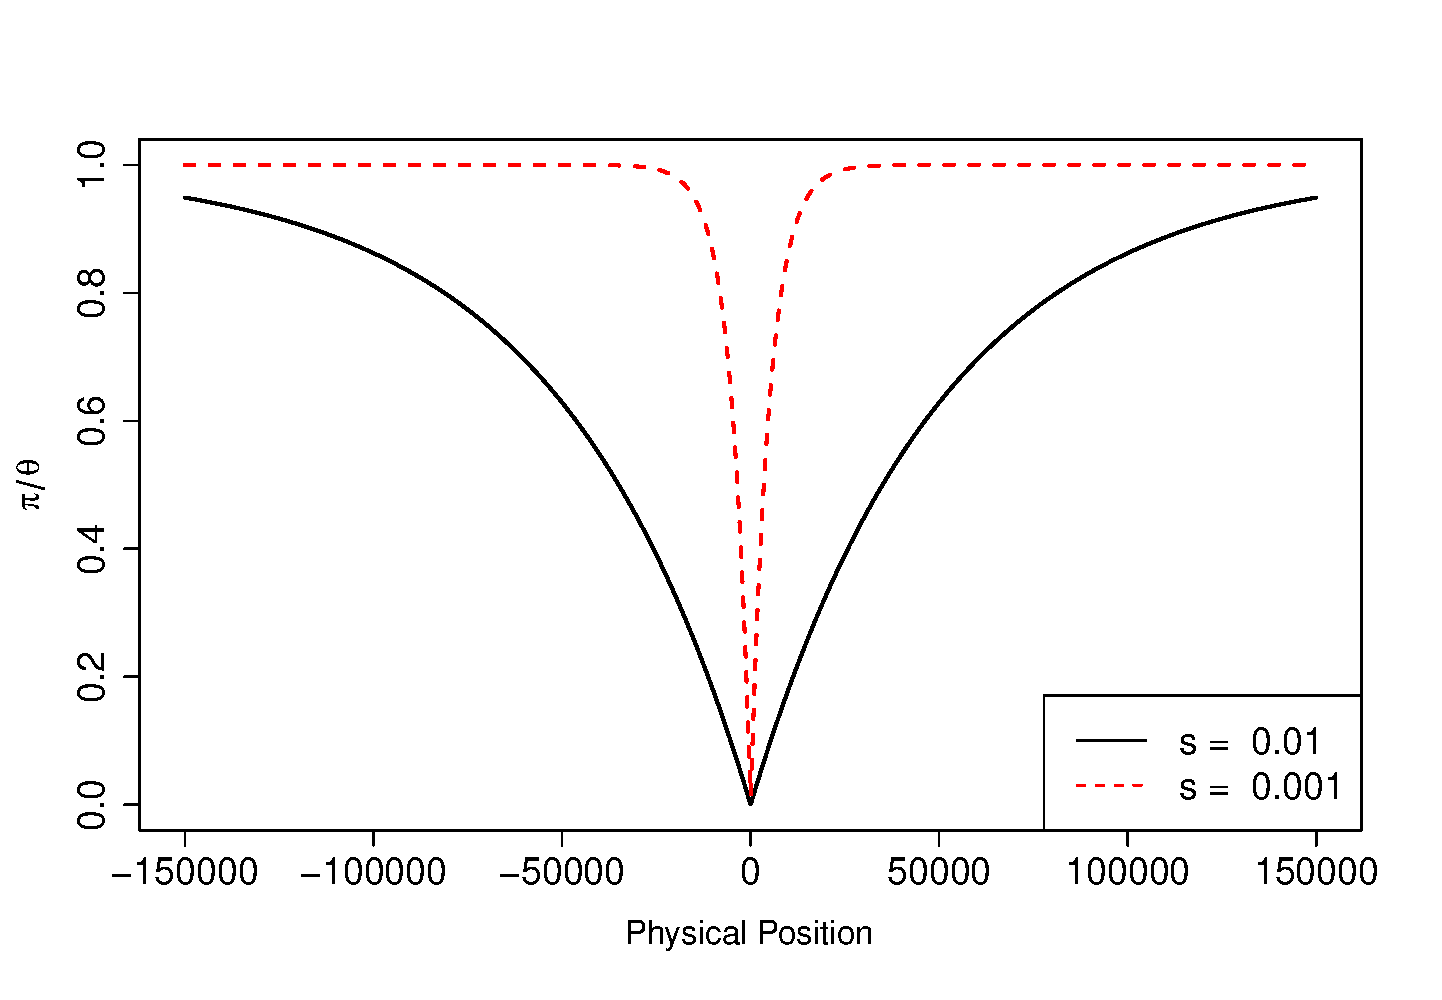
\includegraphics[width=0.5\textwidth]{Figs/hitchhiking_reduction.eps}
\end{center}
\caption{Reduction in diversity compared to its neutral expectation as
a function of the distance away from a site where a selected allele
has just gone to fixation. The recombination rate is $r_{BP}= 1\times
10^{-8}$.} \label{fig:hitchhiking_reduction}
\end{figure}

\subsection{A simple recurrent model of selective sweeps}
We sample a pair of neutral alleles at a locus a genetic distance $r$ away from a locus where
sweeps are initiated within the population at some very low rate $\nu$
per generation. The waiting time between sweeps
at our locus is exponential $\sim Exp(\nu)$. Each sweep rapidly transits through the population in $\tau$
generations, such that each sweep is finished long before the next
sweep ($\tau \ll 1/\nu$). \\

As before our chance that our neutral lineage fails to recombine
off the sweep is $p_{NR}$, such that the probability that
our pair of lineages are forced to coalesce by a sweep $e^{-r \tau}$. Our
lineages therefore have a very low probability
\begin{equation}
\nu e^{-r \tau}
\end{equation}
of being forced to coalesce by a sweep per generation. In addition of
lineages can coalesce at a neutral rate of $1/(2N)$. Thus the average
waiting time till a coalescent event between our neutral pair of
lineages due to either a sweep or a neutral coalescent event is
\begin{equation}
\E(T_2) = \frac{1}{\nu e^{-r \tau} + 1/(2N)}
\end{equation}

Now imagine that the sweeps don't occur at a fixed location with
respect to our locus of interest, but now occur uniformly at random
across our sequence. The sweeps are initiated at a very low rate of
$\nu_{BP}$ per basepair per generation. The rate of coalescent due to
sweeps at a locus $\ell$ basepairs away from our neutral loci is
$\nu_{BP} e^{-r_{BP} \ell \tau}$. If our neutral locus is in the
middle of a chromosome that stretches $L$ basepairs in either direction
the total rate of sweeps per generation that force our pair of lineages to coalesce is
\begin{equation}
2\int_0^{L} \nu_{BP} e^{-r_{BP} \ell \tau} d \ell =
\frac{\nu_{BP}}{r_{BP} \tau} \left(1-e^{-r_{BP} \tau L} \right)
\end{equation}
so that if $L$ is very large ($r_{BP} \tau L \gg 1$) the rate of coalesce per
generation due to sweeps is $\frac{2\nu_{BP}}{r_{BP} \tau}$. The total rate
of coalescence for a pair of lineages per generation is then
\begin{equation}
\frac{2\nu_{BP}}{r_{BP} \tau}+\frac{1}{2N}
\end{equation}
So our average time till a pair of lineages coalesce is
\begin{equation}
\E(T_2) = \frac{1}{\frac{2\nu_{BP}}{r_{BP} \tau}+\frac{1}{2N}} = \frac{r_{BP}2N}{\frac{4N\nu_{BP}}{ \tau}+r_{BP}}
\end{equation}
such that our expected pairwise diversity ($\pi=2\mu\E(T_2)$) in a region of
recombination rate $r_{BP}$ that experiences sweeps at rate $\nu_{BP}$
is  
\begin{equation}
\E(\pi) = \theta \frac{r_{BP}}{\frac{4N\nu_{BP}}{ \tau}+r_{BP}} \label{eqn:pi_GW_HH}
\end{equation}


\begin{figure}
\begin{center}
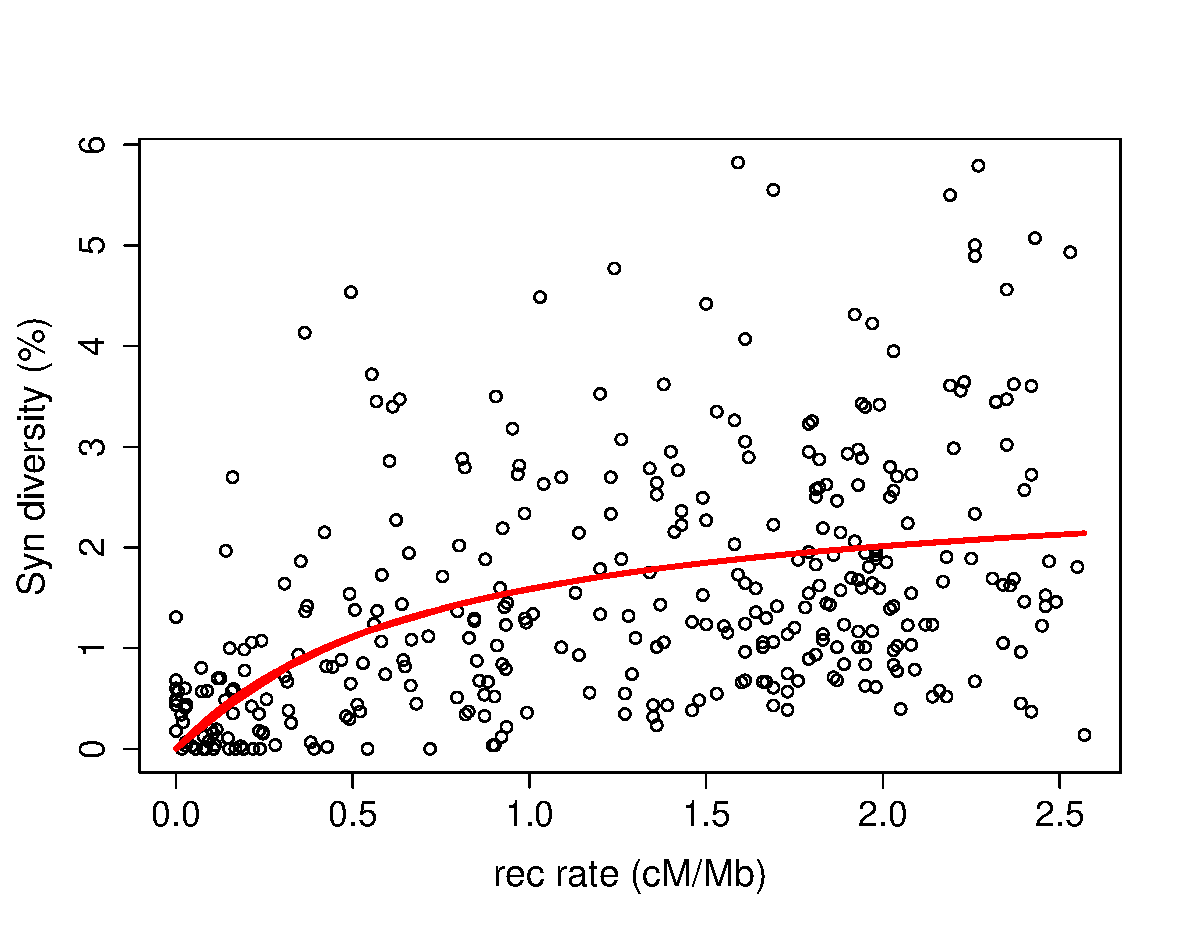
\includegraphics[width=0.5\textwidth]{Figs/Genomewide_HH.eps}
\end{center}
\caption{The relationship between (sex-averaged) recombination rate and synonymous
  site pairwise diversity ($\pi$) in {\it Drosophila melanogaster}
  using the data of Shapiro et al. 07 (kindly provided by Peter
  Andolfatto, see Sella et al. 09 for details). The curve is the
  predicted relationship between $\pi$ and recombination rate obtained
  by fitting equation \eqref{eqn:pi_GW_HH} to this data 
 using non-linear least squares via the {\tt nls()} function in {\tt R}.} \label{fig:GW_hitchhiking_reduction}
\end{figure}


\end{document}
